% Options for packages loaded elsewhere
\PassOptionsToPackage{unicode}{hyperref}
\PassOptionsToPackage{hyphens}{url}
\PassOptionsToPackage{dvipsnames,svgnames,x11names}{xcolor}
%
\documentclass[
  letterpaper,
  DIV=11,
  numbers=noendperiod]{scrartcl}

\usepackage{amsmath,amssymb}
\usepackage{iftex}
\ifPDFTeX
  \usepackage[T1]{fontenc}
  \usepackage[utf8]{inputenc}
  \usepackage{textcomp} % provide euro and other symbols
\else % if luatex or xetex
  \usepackage{unicode-math}
  \defaultfontfeatures{Scale=MatchLowercase}
  \defaultfontfeatures[\rmfamily]{Ligatures=TeX,Scale=1}
\fi
\usepackage{lmodern}
\ifPDFTeX\else  
    % xetex/luatex font selection
\fi
% Use upquote if available, for straight quotes in verbatim environments
\IfFileExists{upquote.sty}{\usepackage{upquote}}{}
\IfFileExists{microtype.sty}{% use microtype if available
  \usepackage[]{microtype}
  \UseMicrotypeSet[protrusion]{basicmath} % disable protrusion for tt fonts
}{}
\makeatletter
\@ifundefined{KOMAClassName}{% if non-KOMA class
  \IfFileExists{parskip.sty}{%
    \usepackage{parskip}
  }{% else
    \setlength{\parindent}{0pt}
    \setlength{\parskip}{6pt plus 2pt minus 1pt}}
}{% if KOMA class
  \KOMAoptions{parskip=half}}
\makeatother
\usepackage{xcolor}
\setlength{\emergencystretch}{3em} % prevent overfull lines
\setcounter{secnumdepth}{-\maxdimen} % remove section numbering
% Make \paragraph and \subparagraph free-standing
\makeatletter
\ifx\paragraph\undefined\else
  \let\oldparagraph\paragraph
  \renewcommand{\paragraph}{
    \@ifstar
      \xxxParagraphStar
      \xxxParagraphNoStar
  }
  \newcommand{\xxxParagraphStar}[1]{\oldparagraph*{#1}\mbox{}}
  \newcommand{\xxxParagraphNoStar}[1]{\oldparagraph{#1}\mbox{}}
\fi
\ifx\subparagraph\undefined\else
  \let\oldsubparagraph\subparagraph
  \renewcommand{\subparagraph}{
    \@ifstar
      \xxxSubParagraphStar
      \xxxSubParagraphNoStar
  }
  \newcommand{\xxxSubParagraphStar}[1]{\oldsubparagraph*{#1}\mbox{}}
  \newcommand{\xxxSubParagraphNoStar}[1]{\oldsubparagraph{#1}\mbox{}}
\fi
\makeatother

\usepackage{color}
\usepackage{fancyvrb}
\newcommand{\VerbBar}{|}
\newcommand{\VERB}{\Verb[commandchars=\\\{\}]}
\DefineVerbatimEnvironment{Highlighting}{Verbatim}{commandchars=\\\{\}}
% Add ',fontsize=\small' for more characters per line
\usepackage{framed}
\definecolor{shadecolor}{RGB}{241,243,245}
\newenvironment{Shaded}{\begin{snugshade}}{\end{snugshade}}
\newcommand{\AlertTok}[1]{\textcolor[rgb]{0.68,0.00,0.00}{#1}}
\newcommand{\AnnotationTok}[1]{\textcolor[rgb]{0.37,0.37,0.37}{#1}}
\newcommand{\AttributeTok}[1]{\textcolor[rgb]{0.40,0.45,0.13}{#1}}
\newcommand{\BaseNTok}[1]{\textcolor[rgb]{0.68,0.00,0.00}{#1}}
\newcommand{\BuiltInTok}[1]{\textcolor[rgb]{0.00,0.23,0.31}{#1}}
\newcommand{\CharTok}[1]{\textcolor[rgb]{0.13,0.47,0.30}{#1}}
\newcommand{\CommentTok}[1]{\textcolor[rgb]{0.37,0.37,0.37}{#1}}
\newcommand{\CommentVarTok}[1]{\textcolor[rgb]{0.37,0.37,0.37}{\textit{#1}}}
\newcommand{\ConstantTok}[1]{\textcolor[rgb]{0.56,0.35,0.01}{#1}}
\newcommand{\ControlFlowTok}[1]{\textcolor[rgb]{0.00,0.23,0.31}{\textbf{#1}}}
\newcommand{\DataTypeTok}[1]{\textcolor[rgb]{0.68,0.00,0.00}{#1}}
\newcommand{\DecValTok}[1]{\textcolor[rgb]{0.68,0.00,0.00}{#1}}
\newcommand{\DocumentationTok}[1]{\textcolor[rgb]{0.37,0.37,0.37}{\textit{#1}}}
\newcommand{\ErrorTok}[1]{\textcolor[rgb]{0.68,0.00,0.00}{#1}}
\newcommand{\ExtensionTok}[1]{\textcolor[rgb]{0.00,0.23,0.31}{#1}}
\newcommand{\FloatTok}[1]{\textcolor[rgb]{0.68,0.00,0.00}{#1}}
\newcommand{\FunctionTok}[1]{\textcolor[rgb]{0.28,0.35,0.67}{#1}}
\newcommand{\ImportTok}[1]{\textcolor[rgb]{0.00,0.46,0.62}{#1}}
\newcommand{\InformationTok}[1]{\textcolor[rgb]{0.37,0.37,0.37}{#1}}
\newcommand{\KeywordTok}[1]{\textcolor[rgb]{0.00,0.23,0.31}{\textbf{#1}}}
\newcommand{\NormalTok}[1]{\textcolor[rgb]{0.00,0.23,0.31}{#1}}
\newcommand{\OperatorTok}[1]{\textcolor[rgb]{0.37,0.37,0.37}{#1}}
\newcommand{\OtherTok}[1]{\textcolor[rgb]{0.00,0.23,0.31}{#1}}
\newcommand{\PreprocessorTok}[1]{\textcolor[rgb]{0.68,0.00,0.00}{#1}}
\newcommand{\RegionMarkerTok}[1]{\textcolor[rgb]{0.00,0.23,0.31}{#1}}
\newcommand{\SpecialCharTok}[1]{\textcolor[rgb]{0.37,0.37,0.37}{#1}}
\newcommand{\SpecialStringTok}[1]{\textcolor[rgb]{0.13,0.47,0.30}{#1}}
\newcommand{\StringTok}[1]{\textcolor[rgb]{0.13,0.47,0.30}{#1}}
\newcommand{\VariableTok}[1]{\textcolor[rgb]{0.07,0.07,0.07}{#1}}
\newcommand{\VerbatimStringTok}[1]{\textcolor[rgb]{0.13,0.47,0.30}{#1}}
\newcommand{\WarningTok}[1]{\textcolor[rgb]{0.37,0.37,0.37}{\textit{#1}}}

\providecommand{\tightlist}{%
  \setlength{\itemsep}{0pt}\setlength{\parskip}{0pt}}\usepackage{longtable,booktabs,array}
\usepackage{calc} % for calculating minipage widths
% Correct order of tables after \paragraph or \subparagraph
\usepackage{etoolbox}
\makeatletter
\patchcmd\longtable{\par}{\if@noskipsec\mbox{}\fi\par}{}{}
\makeatother
% Allow footnotes in longtable head/foot
\IfFileExists{footnotehyper.sty}{\usepackage{footnotehyper}}{\usepackage{footnote}}
\makesavenoteenv{longtable}
\usepackage{graphicx}
\makeatletter
\def\maxwidth{\ifdim\Gin@nat@width>\linewidth\linewidth\else\Gin@nat@width\fi}
\def\maxheight{\ifdim\Gin@nat@height>\textheight\textheight\else\Gin@nat@height\fi}
\makeatother
% Scale images if necessary, so that they will not overflow the page
% margins by default, and it is still possible to overwrite the defaults
% using explicit options in \includegraphics[width, height, ...]{}
\setkeys{Gin}{width=\maxwidth,height=\maxheight,keepaspectratio}
% Set default figure placement to htbp
\makeatletter
\def\fps@figure{htbp}
\makeatother

\KOMAoption{captions}{tableheading}
\makeatletter
\@ifpackageloaded{caption}{}{\usepackage{caption}}
\AtBeginDocument{%
\ifdefined\contentsname
  \renewcommand*\contentsname{Table of contents}
\else
  \newcommand\contentsname{Table of contents}
\fi
\ifdefined\listfigurename
  \renewcommand*\listfigurename{List of Figures}
\else
  \newcommand\listfigurename{List of Figures}
\fi
\ifdefined\listtablename
  \renewcommand*\listtablename{List of Tables}
\else
  \newcommand\listtablename{List of Tables}
\fi
\ifdefined\figurename
  \renewcommand*\figurename{Figure}
\else
  \newcommand\figurename{Figure}
\fi
\ifdefined\tablename
  \renewcommand*\tablename{Table}
\else
  \newcommand\tablename{Table}
\fi
}
\@ifpackageloaded{float}{}{\usepackage{float}}
\floatstyle{ruled}
\@ifundefined{c@chapter}{\newfloat{codelisting}{h}{lop}}{\newfloat{codelisting}{h}{lop}[chapter]}
\floatname{codelisting}{Listing}
\newcommand*\listoflistings{\listof{codelisting}{List of Listings}}
\makeatother
\makeatletter
\makeatother
\makeatletter
\@ifpackageloaded{caption}{}{\usepackage{caption}}
\@ifpackageloaded{subcaption}{}{\usepackage{subcaption}}
\makeatother
\ifLuaTeX
  \usepackage{selnolig}  % disable illegal ligatures
\fi
\usepackage{bookmark}

\IfFileExists{xurl.sty}{\usepackage{xurl}}{} % add URL line breaks if available
\urlstyle{same} % disable monospaced font for URLs
\hypersetup{
  pdftitle={Housing Wealth Analysis: Black vs White Households (1989-2016)},
  colorlinks=true,
  linkcolor={blue},
  filecolor={Maroon},
  citecolor={Blue},
  urlcolor={Blue},
  pdfcreator={LaTeX via pandoc}}

\title{Housing Wealth Analysis: Black vs White Households (1989-2016)}
\author{}
\date{}

\begin{document}
\maketitle

\begin{Shaded}
\begin{Highlighting}[]
\ImportTok{import}\NormalTok{ pandas }\ImportTok{as}\NormalTok{ pd}

\NormalTok{df }\OperatorTok{=}\NormalTok{ pd.read\_csv(}\VerbatimStringTok{r\textquotesingle{}C:\textbackslash{}Users\textbackslash{}clint\textbackslash{}Desktop\textbackslash{}Booth RA\textbackslash{}RA\_21\_22.csv\textquotesingle{}}\NormalTok{)}
\NormalTok{df}
\end{Highlighting}
\end{Shaded}

\begin{longtable}[]{@{}llllllllllll@{}}
\toprule\noalign{}
& weight & year & age & sex & education & race & asset\_total &
asset\_housing & debt\_total & debt\_housing & income \\
\midrule\noalign{}
\endhead
\bottomrule\noalign{}
\endlastfoot
0 & 6859.959728 & 1989 & 35 & female & no college & white & 3731.72 &
0.00 & 1530.01 & 0.00 & 9737.17 \\
1 & 7375.788638 & 1989 & 35 & female & no college & black & 0.00 & 0.00
& 0.00 & 0.00 & 11684.60 \\
2 & 4193.294199 & 1989 & 40 & male & no college & other & 216439.77 &
139939.51 & 26681.80 & 18658.60 & 83739.63 \\
3 & 4743.208024 & 1989 & 51 & female & no college & black & 40060.02 &
18658.60 & 26383.26 & 5597.58 & 19474.33 \\
4 & 5971.319496 & 1989 & 28 & male & no college & black & 35675.24 &
33585.48 & 27987.90 & 20524.46 & 35053.80 \\
... & ... & ... & ... & ... & ... & ... & ... & ... & ... & ... & ... \\
47771 & 3033.103970 & 2016 & 43 & male & some college & white &
253300.00 & 0.00 & 96500.00 & 0.00 & 113415.28 \\
47772 & 5721.988043 & 2016 & 67 & male & some college & white &
279400.00 & 120000.00 & 15000.00 & 0.00 & 109364.73 \\
47773 & 4824.390087 & 2016 & 60 & male & college degree & white &
1500.00 & 0.00 & 35000.00 & 0.00 & 40505.46 \\
47774 & 4132.549093 & 2016 & 48 & female & no college & white & 4430.00
& 0.00 & 100.00 & 0.00 & 23290.64 \\
47775 & 4461.752118 & 2016 & 29 & male & some college & white & 92600.00
& 0.00 & 15900.00 & 0.00 & 21265.36 \\
\end{longtable}

\begin{Shaded}
\begin{Highlighting}[]
\CommentTok{\# COMPREHENSIVE DATA QUALITY ASSESSMENT}
\BuiltInTok{print}\NormalTok{(}\StringTok{"=== DATA QUALITY ASSESSMENT ===}\CharTok{\textbackslash{}n}\StringTok{"}\NormalTok{)}

\CommentTok{\# 1. Basic dataset information}
\BuiltInTok{print}\NormalTok{(}\StringTok{"1. DATASET OVERVIEW:"}\NormalTok{)}
\BuiltInTok{print}\NormalTok{(}\SpecialStringTok{f"   Shape: }\SpecialCharTok{\{}\NormalTok{df}\SpecialCharTok{.}\NormalTok{shape[}\DecValTok{0}\NormalTok{]}\SpecialCharTok{:,\}}\SpecialStringTok{ rows × }\SpecialCharTok{\{}\NormalTok{df}\SpecialCharTok{.}\NormalTok{shape[}\DecValTok{1}\NormalTok{]}\SpecialCharTok{\}}\SpecialStringTok{ columns"}\NormalTok{)}
\BuiltInTok{print}\NormalTok{(}\SpecialStringTok{f"   Memory usage: }\SpecialCharTok{\{}\NormalTok{df}\SpecialCharTok{.}\NormalTok{memory\_usage(deep}\OperatorTok{=}\VariableTok{True}\NormalTok{)}\SpecialCharTok{.}\BuiltInTok{sum}\NormalTok{() }\OperatorTok{/} \DecValTok{1024}\OperatorTok{**}\DecValTok{2}\SpecialCharTok{:.2f\}}\SpecialStringTok{ MB"}\NormalTok{)}
\BuiltInTok{print}\NormalTok{(}\SpecialStringTok{f"   Columns: }\SpecialCharTok{\{}\BuiltInTok{list}\NormalTok{(df.columns)}\SpecialCharTok{\}}\SpecialStringTok{"}\NormalTok{)}

\CommentTok{\# 2. Missing values analysis}
\BuiltInTok{print}\NormalTok{(}\StringTok{"}\CharTok{\textbackslash{}n}\StringTok{2. MISSING VALUES CHECK:"}\NormalTok{)}
\NormalTok{missing\_summary }\OperatorTok{=}\NormalTok{ df.isnull().}\BuiltInTok{sum}\NormalTok{()}
\NormalTok{missing\_pct }\OperatorTok{=}\NormalTok{ (df.isnull().}\BuiltInTok{sum}\NormalTok{() }\OperatorTok{/} \BuiltInTok{len}\NormalTok{(df)) }\OperatorTok{*} \DecValTok{100}
\NormalTok{missing\_df }\OperatorTok{=}\NormalTok{ pd.DataFrame(\{}
    \StringTok{\textquotesingle{}Missing\_Count\textquotesingle{}}\NormalTok{: missing\_summary,}
    \StringTok{\textquotesingle{}Missing\_Percentage\textquotesingle{}}\NormalTok{: missing\_pct}
\NormalTok{\})}
\BuiltInTok{print}\NormalTok{(missing\_df[missing\_df[}\StringTok{\textquotesingle{}Missing\_Count\textquotesingle{}}\NormalTok{] }\OperatorTok{\textgreater{}} \DecValTok{0}\NormalTok{])}
\ControlFlowTok{if}\NormalTok{ missing\_df[}\StringTok{\textquotesingle{}Missing\_Count\textquotesingle{}}\NormalTok{].}\BuiltInTok{sum}\NormalTok{() }\OperatorTok{==} \DecValTok{0}\NormalTok{:}
    \BuiltInTok{print}\NormalTok{(}\StringTok{"   ✓ No missing values found"}\NormalTok{)}

\CommentTok{\# 3. Data types and value ranges}
\BuiltInTok{print}\NormalTok{(}\StringTok{"}\CharTok{\textbackslash{}n}\StringTok{3. DATA TYPES AND RANGES:"}\NormalTok{)}
\ControlFlowTok{for}\NormalTok{ col }\KeywordTok{in}\NormalTok{ df.columns:}
\NormalTok{    dtype }\OperatorTok{=}\NormalTok{ df[col].dtype}
    \ControlFlowTok{if}\NormalTok{ df[col].dtype }\KeywordTok{in}\NormalTok{ [}\StringTok{\textquotesingle{}int64\textquotesingle{}}\NormalTok{, }\StringTok{\textquotesingle{}float64\textquotesingle{}}\NormalTok{]:}
\NormalTok{        min\_val }\OperatorTok{=}\NormalTok{ df[col].}\BuiltInTok{min}\NormalTok{()}
\NormalTok{        max\_val }\OperatorTok{=}\NormalTok{ df[col].}\BuiltInTok{max}\NormalTok{()}
        \BuiltInTok{print}\NormalTok{(}\SpecialStringTok{f"   }\SpecialCharTok{\{}\NormalTok{col}\SpecialCharTok{\}}\SpecialStringTok{: }\SpecialCharTok{\{}\NormalTok{dtype}\SpecialCharTok{\}}\SpecialStringTok{ | Range: }\SpecialCharTok{\{}\NormalTok{min\_val}\SpecialCharTok{:,.2f\}}\SpecialStringTok{ to }\SpecialCharTok{\{}\NormalTok{max\_val}\SpecialCharTok{:,.2f\}}\SpecialStringTok{"}\NormalTok{)}
    \ControlFlowTok{else}\NormalTok{:}
\NormalTok{        unique\_count }\OperatorTok{=}\NormalTok{ df[col].nunique()}
        \BuiltInTok{print}\NormalTok{(}\SpecialStringTok{f"   }\SpecialCharTok{\{}\NormalTok{col}\SpecialCharTok{\}}\SpecialStringTok{: }\SpecialCharTok{\{}\NormalTok{dtype}\SpecialCharTok{\}}\SpecialStringTok{ | }\SpecialCharTok{\{}\NormalTok{unique\_count}\SpecialCharTok{\}}\SpecialStringTok{ unique values"}\NormalTok{)}

\CommentTok{\# 4. Check for negative values in financial columns}
\BuiltInTok{print}\NormalTok{(}\StringTok{"}\CharTok{\textbackslash{}n}\StringTok{4. NEGATIVE VALUES CHECK:"}\NormalTok{)}
\NormalTok{financial\_cols }\OperatorTok{=}\NormalTok{ [}\StringTok{\textquotesingle{}weight\textquotesingle{}}\NormalTok{, }\StringTok{\textquotesingle{}asset\_total\textquotesingle{}}\NormalTok{, }\StringTok{\textquotesingle{}asset\_housing\textquotesingle{}}\NormalTok{, }\StringTok{\textquotesingle{}debt\_total\textquotesingle{}}\NormalTok{, }\StringTok{\textquotesingle{}debt\_housing\textquotesingle{}}\NormalTok{, }\StringTok{\textquotesingle{}income\textquotesingle{}}\NormalTok{, }\StringTok{\textquotesingle{}wealth\textquotesingle{}}\NormalTok{]}
\ControlFlowTok{for}\NormalTok{ col }\KeywordTok{in}\NormalTok{ financial\_cols:}
    \ControlFlowTok{if}\NormalTok{ col }\KeywordTok{in}\NormalTok{ df.columns:}
\NormalTok{        negative\_count }\OperatorTok{=}\NormalTok{ (df[col] }\OperatorTok{\textless{}} \DecValTok{0}\NormalTok{).}\BuiltInTok{sum}\NormalTok{()}
\NormalTok{        negative\_pct }\OperatorTok{=}\NormalTok{ (negative\_count }\OperatorTok{/} \BuiltInTok{len}\NormalTok{(df)) }\OperatorTok{*} \DecValTok{100}
        \ControlFlowTok{if}\NormalTok{ negative\_count }\OperatorTok{\textgreater{}} \DecValTok{0}\NormalTok{:}
            \BuiltInTok{print}\NormalTok{(}\SpecialStringTok{f"   ⚠️ }\SpecialCharTok{\{}\NormalTok{col}\SpecialCharTok{\}}\SpecialStringTok{: }\SpecialCharTok{\{}\NormalTok{negative\_count}\SpecialCharTok{:,\}}\SpecialStringTok{ negative values (}\SpecialCharTok{\{}\NormalTok{negative\_pct}\SpecialCharTok{:.2f\}}\SpecialStringTok{\%)"}\NormalTok{)}
        \ControlFlowTok{else}\NormalTok{:}
            \BuiltInTok{print}\NormalTok{(}\SpecialStringTok{f"   ✓ }\SpecialCharTok{\{}\NormalTok{col}\SpecialCharTok{\}}\SpecialStringTok{: No negative values"}\NormalTok{)}

\CommentTok{\# 5. Outlier detection using IQR method}
\BuiltInTok{print}\NormalTok{(}\StringTok{"}\CharTok{\textbackslash{}n}\StringTok{5. OUTLIER DETECTION (IQR Method):"}\NormalTok{)}
\ControlFlowTok{for}\NormalTok{ col }\KeywordTok{in}\NormalTok{ financial\_cols:}
    \ControlFlowTok{if}\NormalTok{ col }\KeywordTok{in}\NormalTok{ df.columns }\KeywordTok{and}\NormalTok{ df[col].dtype }\KeywordTok{in}\NormalTok{ [}\StringTok{\textquotesingle{}int64\textquotesingle{}}\NormalTok{, }\StringTok{\textquotesingle{}float64\textquotesingle{}}\NormalTok{]:}
\NormalTok{        Q1 }\OperatorTok{=}\NormalTok{ df[col].quantile(}\FloatTok{0.25}\NormalTok{)}
\NormalTok{        Q3 }\OperatorTok{=}\NormalTok{ df[col].quantile(}\FloatTok{0.75}\NormalTok{)}
\NormalTok{        IQR }\OperatorTok{=}\NormalTok{ Q3 }\OperatorTok{{-}}\NormalTok{ Q1}
\NormalTok{        lower\_bound }\OperatorTok{=}\NormalTok{ Q1 }\OperatorTok{{-}} \FloatTok{1.5} \OperatorTok{*}\NormalTok{ IQR}
\NormalTok{        upper\_bound }\OperatorTok{=}\NormalTok{ Q3 }\OperatorTok{+} \FloatTok{1.5} \OperatorTok{*}\NormalTok{ IQR}
\NormalTok{        outliers }\OperatorTok{=}\NormalTok{ ((df[col] }\OperatorTok{\textless{}}\NormalTok{ lower\_bound) }\OperatorTok{|}\NormalTok{ (df[col] }\OperatorTok{\textgreater{}}\NormalTok{ upper\_bound)).}\BuiltInTok{sum}\NormalTok{()}
\NormalTok{        outlier\_pct }\OperatorTok{=}\NormalTok{ (outliers }\OperatorTok{/} \BuiltInTok{len}\NormalTok{(df)) }\OperatorTok{*} \DecValTok{100}
        \BuiltInTok{print}\NormalTok{(}\SpecialStringTok{f"   }\SpecialCharTok{\{}\NormalTok{col}\SpecialCharTok{\}}\SpecialStringTok{: }\SpecialCharTok{\{}\NormalTok{outliers}\SpecialCharTok{:,\}}\SpecialStringTok{ outliers (}\SpecialCharTok{\{}\NormalTok{outlier\_pct}\SpecialCharTok{:.1f\}}\SpecialStringTok{\%) | Bounds: [}\SpecialCharTok{\{}\NormalTok{lower\_bound}\SpecialCharTok{:,.0f\}}\SpecialStringTok{, }\SpecialCharTok{\{}\NormalTok{upper\_bound}\SpecialCharTok{:,.0f\}}\SpecialStringTok{]"}\NormalTok{)}

\CommentTok{\# 6. Categorical variables validation}
\BuiltInTok{print}\NormalTok{(}\StringTok{"}\CharTok{\textbackslash{}n}\StringTok{6. CATEGORICAL VARIABLES:"}\NormalTok{)}
\NormalTok{categorical\_cols }\OperatorTok{=}\NormalTok{ [}\StringTok{\textquotesingle{}race\textquotesingle{}}\NormalTok{, }\StringTok{\textquotesingle{}education\textquotesingle{}}\NormalTok{, }\StringTok{\textquotesingle{}sex\textquotesingle{}}\NormalTok{]}
\ControlFlowTok{for}\NormalTok{ col }\KeywordTok{in}\NormalTok{ categorical\_cols:}
    \ControlFlowTok{if}\NormalTok{ col }\KeywordTok{in}\NormalTok{ df.columns:}
\NormalTok{        value\_counts }\OperatorTok{=}\NormalTok{ df[col].value\_counts()}
        \BuiltInTok{print}\NormalTok{(}\SpecialStringTok{f"   }\SpecialCharTok{\{}\NormalTok{col}\SpecialCharTok{\}}\SpecialStringTok{:"}\NormalTok{)}
        \ControlFlowTok{for}\NormalTok{ value, count }\KeywordTok{in}\NormalTok{ value\_counts.items():}
\NormalTok{            pct }\OperatorTok{=}\NormalTok{ (count }\OperatorTok{/} \BuiltInTok{len}\NormalTok{(df)) }\OperatorTok{*} \DecValTok{100}
            \BuiltInTok{print}\NormalTok{(}\SpecialStringTok{f"     {-} }\SpecialCharTok{\{}\NormalTok{value}\SpecialCharTok{\}}\SpecialStringTok{: }\SpecialCharTok{\{}\NormalTok{count}\SpecialCharTok{:,\}}\SpecialStringTok{ (}\SpecialCharTok{\{}\NormalTok{pct}\SpecialCharTok{:.1f\}}\SpecialStringTok{\%)"}\NormalTok{)}

\CommentTok{\# 7. Year distribution}
\BuiltInTok{print}\NormalTok{(}\StringTok{"}\CharTok{\textbackslash{}n}\StringTok{7. YEAR DISTRIBUTION:"}\NormalTok{)}
\ControlFlowTok{if} \StringTok{\textquotesingle{}year\textquotesingle{}} \KeywordTok{in}\NormalTok{ df.columns:}
\NormalTok{    year\_counts }\OperatorTok{=}\NormalTok{ df[}\StringTok{\textquotesingle{}year\textquotesingle{}}\NormalTok{].value\_counts().sort\_index()}
    \ControlFlowTok{for}\NormalTok{ year, count }\KeywordTok{in}\NormalTok{ year\_counts.items():}
\NormalTok{        pct }\OperatorTok{=}\NormalTok{ (count }\OperatorTok{/} \BuiltInTok{len}\NormalTok{(df)) }\OperatorTok{*} \DecValTok{100}
        \BuiltInTok{print}\NormalTok{(}\SpecialStringTok{f"   }\SpecialCharTok{\{}\NormalTok{year}\SpecialCharTok{\}}\SpecialStringTok{: }\SpecialCharTok{\{}\NormalTok{count}\SpecialCharTok{:,\}}\SpecialStringTok{ observations (}\SpecialCharTok{\{}\NormalTok{pct}\SpecialCharTok{:.1f\}}\SpecialStringTok{\%)"}\NormalTok{)}

\CommentTok{\# 8. Logical consistency checks}
\BuiltInTok{print}\NormalTok{(}\StringTok{"}\CharTok{\textbackslash{}n}\StringTok{8. LOGICAL CONSISTENCY CHECKS:"}\NormalTok{)}

\CommentTok{\# Check if housing assets \textless{}= total assets}
\ControlFlowTok{if} \StringTok{\textquotesingle{}asset\_housing\textquotesingle{}} \KeywordTok{in}\NormalTok{ df.columns }\KeywordTok{and} \StringTok{\textquotesingle{}asset\_total\textquotesingle{}} \KeywordTok{in}\NormalTok{ df.columns:}
\NormalTok{    housing\_gt\_total }\OperatorTok{=}\NormalTok{ (df[}\StringTok{\textquotesingle{}asset\_housing\textquotesingle{}}\NormalTok{] }\OperatorTok{\textgreater{}}\NormalTok{ df[}\StringTok{\textquotesingle{}asset\_total\textquotesingle{}}\NormalTok{]).}\BuiltInTok{sum}\NormalTok{()}
    \ControlFlowTok{if}\NormalTok{ housing\_gt\_total }\OperatorTok{\textgreater{}} \DecValTok{0}\NormalTok{:}
        \BuiltInTok{print}\NormalTok{(}\SpecialStringTok{f"   ⚠️ }\SpecialCharTok{\{}\NormalTok{housing\_gt\_total}\SpecialCharTok{:,\}}\SpecialStringTok{ cases where housing assets \textgreater{} total assets"}\NormalTok{)}
    \ControlFlowTok{else}\NormalTok{:}
        \BuiltInTok{print}\NormalTok{(}\StringTok{"   ✓ Housing assets ≤ total assets for all cases"}\NormalTok{)}

\CommentTok{\# Check if housing debt \textless{}= total debt}
\ControlFlowTok{if} \StringTok{\textquotesingle{}debt\_housing\textquotesingle{}} \KeywordTok{in}\NormalTok{ df.columns }\KeywordTok{and} \StringTok{\textquotesingle{}debt\_total\textquotesingle{}} \KeywordTok{in}\NormalTok{ df.columns:}
\NormalTok{    housing\_debt\_gt\_total }\OperatorTok{=}\NormalTok{ (df[}\StringTok{\textquotesingle{}debt\_housing\textquotesingle{}}\NormalTok{] }\OperatorTok{\textgreater{}}\NormalTok{ df[}\StringTok{\textquotesingle{}debt\_total\textquotesingle{}}\NormalTok{]).}\BuiltInTok{sum}\NormalTok{()}
    \ControlFlowTok{if}\NormalTok{ housing\_debt\_gt\_total }\OperatorTok{\textgreater{}} \DecValTok{0}\NormalTok{:}
        \BuiltInTok{print}\NormalTok{(}\SpecialStringTok{f"   ⚠️ }\SpecialCharTok{\{}\NormalTok{housing\_debt\_gt\_total}\SpecialCharTok{:,\}}\SpecialStringTok{ cases where housing debt \textgreater{} total debt"}\NormalTok{)}
    \ControlFlowTok{else}\NormalTok{:}
        \BuiltInTok{print}\NormalTok{(}\StringTok{"   ✓ Housing debt ≤ total debt for all cases"}\NormalTok{)}

\CommentTok{\# Check if wealth calculation is consistent}
\ControlFlowTok{if} \StringTok{\textquotesingle{}wealth\textquotesingle{}} \KeywordTok{in}\NormalTok{ df.columns:}
\NormalTok{    calculated\_wealth }\OperatorTok{=}\NormalTok{ df[}\StringTok{\textquotesingle{}asset\_total\textquotesingle{}}\NormalTok{] }\OperatorTok{+}\NormalTok{ df[}\StringTok{\textquotesingle{}asset\_housing\textquotesingle{}}\NormalTok{] }\OperatorTok{{-}}\NormalTok{ df[}\StringTok{\textquotesingle{}debt\_total\textquotesingle{}}\NormalTok{] }\OperatorTok{{-}}\NormalTok{ df[}\StringTok{\textquotesingle{}debt\_housing\textquotesingle{}}\NormalTok{]}
\NormalTok{    wealth\_inconsistent }\OperatorTok{=}\NormalTok{ (}\BuiltInTok{abs}\NormalTok{(df[}\StringTok{\textquotesingle{}wealth\textquotesingle{}}\NormalTok{] }\OperatorTok{{-}}\NormalTok{ calculated\_wealth) }\OperatorTok{\textgreater{}} \FloatTok{0.01}\NormalTok{).}\BuiltInTok{sum}\NormalTok{()}
    \ControlFlowTok{if}\NormalTok{ wealth\_inconsistent }\OperatorTok{\textgreater{}} \DecValTok{0}\NormalTok{:}
        \BuiltInTok{print}\NormalTok{(}\SpecialStringTok{f"   ⚠️ }\SpecialCharTok{\{}\NormalTok{wealth\_inconsistent}\SpecialCharTok{:,\}}\SpecialStringTok{ cases with inconsistent wealth calculation"}\NormalTok{)}
    \ControlFlowTok{else}\NormalTok{:}
        \BuiltInTok{print}\NormalTok{(}\StringTok{"   ✓ Wealth calculation is consistent"}\NormalTok{)}

\CommentTok{\# 9. Survey weights validation}
\BuiltInTok{print}\NormalTok{(}\StringTok{"}\CharTok{\textbackslash{}n}\StringTok{9. SURVEY WEIGHTS VALIDATION:"}\NormalTok{)}
\ControlFlowTok{if} \StringTok{\textquotesingle{}weight\textquotesingle{}} \KeywordTok{in}\NormalTok{ df.columns:}
\NormalTok{    zero\_weights }\OperatorTok{=}\NormalTok{ (df[}\StringTok{\textquotesingle{}weight\textquotesingle{}}\NormalTok{] }\OperatorTok{==} \DecValTok{0}\NormalTok{).}\BuiltInTok{sum}\NormalTok{()}
\NormalTok{    very\_small\_weights }\OperatorTok{=}\NormalTok{ (df[}\StringTok{\textquotesingle{}weight\textquotesingle{}}\NormalTok{] }\OperatorTok{\textless{}} \DecValTok{1}\NormalTok{).}\BuiltInTok{sum}\NormalTok{()}
\NormalTok{    very\_large\_weights }\OperatorTok{=}\NormalTok{ (df[}\StringTok{\textquotesingle{}weight\textquotesingle{}}\NormalTok{] }\OperatorTok{\textgreater{}} \DecValTok{50000}\NormalTok{).}\BuiltInTok{sum}\NormalTok{()}
    
    \BuiltInTok{print}\NormalTok{(}\SpecialStringTok{f"   Zero weights: }\SpecialCharTok{\{}\NormalTok{zero\_weights}\SpecialCharTok{:,\}}\SpecialStringTok{"}\NormalTok{)}
    \BuiltInTok{print}\NormalTok{(}\SpecialStringTok{f"   Very small weights (\textless{}1): }\SpecialCharTok{\{}\NormalTok{very\_small\_weights}\SpecialCharTok{:,\}}\SpecialStringTok{"}\NormalTok{)}
    \BuiltInTok{print}\NormalTok{(}\SpecialStringTok{f"   Very large weights (\textgreater{}50K): }\SpecialCharTok{\{}\NormalTok{very\_large\_weights}\SpecialCharTok{:,\}}\SpecialStringTok{"}\NormalTok{)}
    \BuiltInTok{print}\NormalTok{(}\SpecialStringTok{f"   Weight statistics: Mean=}\SpecialCharTok{\{}\NormalTok{df[}\StringTok{\textquotesingle{}weight\textquotesingle{}}\NormalTok{]}\SpecialCharTok{.}\NormalTok{mean()}\SpecialCharTok{:.1f\}}\SpecialStringTok{, Median=}\SpecialCharTok{\{}\NormalTok{df[}\StringTok{\textquotesingle{}weight\textquotesingle{}}\NormalTok{]}\SpecialCharTok{.}\NormalTok{median()}\SpecialCharTok{:.1f\}}\SpecialStringTok{"}\NormalTok{)}

\CommentTok{\# 10. Summary}
\BuiltInTok{print}\NormalTok{(}\StringTok{"}\CharTok{\textbackslash{}n}\StringTok{=== DATA QUALITY SUMMARY ==="}\NormalTok{)}
\NormalTok{issues\_found }\OperatorTok{=}\NormalTok{ []}

\ControlFlowTok{if}\NormalTok{ missing\_df[}\StringTok{\textquotesingle{}Missing\_Count\textquotesingle{}}\NormalTok{].}\BuiltInTok{sum}\NormalTok{() }\OperatorTok{\textgreater{}} \DecValTok{0}\NormalTok{:}
\NormalTok{    issues\_found.append(}\StringTok{"Missing values detected"}\NormalTok{)}
    
\ControlFlowTok{if} \BuiltInTok{any}\NormalTok{((df[col] }\OperatorTok{\textless{}} \DecValTok{0}\NormalTok{).}\BuiltInTok{sum}\NormalTok{() }\OperatorTok{\textgreater{}} \DecValTok{0} \ControlFlowTok{for}\NormalTok{ col }\KeywordTok{in}\NormalTok{ financial\_cols }\ControlFlowTok{if}\NormalTok{ col }\KeywordTok{in}\NormalTok{ df.columns):}
\NormalTok{    issues\_found.append(}\StringTok{"Negative values in financial columns"}\NormalTok{)}

\ControlFlowTok{if} \StringTok{\textquotesingle{}asset\_housing\textquotesingle{}} \KeywordTok{in}\NormalTok{ df.columns }\KeywordTok{and} \StringTok{\textquotesingle{}asset\_total\textquotesingle{}} \KeywordTok{in}\NormalTok{ df.columns:}
    \ControlFlowTok{if}\NormalTok{ (df[}\StringTok{\textquotesingle{}asset\_housing\textquotesingle{}}\NormalTok{] }\OperatorTok{\textgreater{}}\NormalTok{ df[}\StringTok{\textquotesingle{}asset\_total\textquotesingle{}}\NormalTok{]).}\BuiltInTok{sum}\NormalTok{() }\OperatorTok{\textgreater{}} \DecValTok{0}\NormalTok{:}
\NormalTok{        issues\_found.append(}\StringTok{"Logical inconsistencies (housing \textgreater{} total assets)"}\NormalTok{)}

\ControlFlowTok{if}\NormalTok{ issues\_found:}
    \BuiltInTok{print}\NormalTok{(}\StringTok{"⚠️ Issues found:"}\NormalTok{)}
    \ControlFlowTok{for}\NormalTok{ issue }\KeywordTok{in}\NormalTok{ issues\_found:}
        \BuiltInTok{print}\NormalTok{(}\SpecialStringTok{f"   {-} }\SpecialCharTok{\{}\NormalTok{issue}\SpecialCharTok{\}}\SpecialStringTok{"}\NormalTok{)}
\ControlFlowTok{else}\NormalTok{:}
    \BuiltInTok{print}\NormalTok{(}\StringTok{"✅ No major data quality issues detected!"}\NormalTok{)}

\BuiltInTok{print}\NormalTok{(}\SpecialStringTok{f"}\CharTok{\textbackslash{}n}\SpecialStringTok{Dataset is ready for analysis with }\SpecialCharTok{\{}\BuiltInTok{len}\NormalTok{(df)}\SpecialCharTok{:,\}}\SpecialStringTok{ observations."}\NormalTok{)}
\end{Highlighting}
\end{Shaded}

\begin{verbatim}
=== DATA QUALITY ASSESSMENT ===

1. DATASET OVERVIEW:
   Shape: 47,776 rows × 11 columns
   Memory usage: 10.60 MB
   Columns: ['weight', 'year', 'age', 'sex', 'education', 'race', 'asset_total', 'asset_housing', 'debt_total', 'debt_housing', 'income']

2. MISSING VALUES CHECK:
Empty DataFrame
Columns: [Missing_Count, Missing_Percentage]
Index: []
   ✓ No missing values found

3. DATA TYPES AND RANGES:
   weight: float64 | Range: 0.20 to 31,115.82
   year: int64 | Range: 1,989.00 to 2,016.00
   age: int64 | Range: 17.00 to 95.00
   sex: object | 2 unique values
   education: object | 3 unique values
   race: object | 4 unique values
   asset_total: float64 | Range: -22,487,306.62 to 2,928,346,179.67
   asset_housing: float64 | Range: 0.00 to 182,642,128.63
   debt_total: float64 | Range: 0.00 to 293,486,997.64
   debt_housing: float64 | Range: 0.00 to 44,821,081.33
   income: float64 | Range: 0.00 to 351,958,858.31

4. NEGATIVE VALUES CHECK:
   ✓ weight: No negative values
   ⚠️ asset_total: 7 negative values (0.01%)
   ✓ asset_housing: No negative values
   ✓ debt_total: No negative values
   ✓ debt_housing: No negative values
   ✓ income: No negative values

5. OUTLIER DETECTION (IQR Method):
   weight: 330 outliers (0.7%) | Bounds: [-4,095, 12,858]
   asset_total: 8,281 outliers (17.3%) | Bounds: [-2,215,818, 3,831,215]
   asset_housing: 5,405 outliers (11.3%) | Bounds: [-651,383, 1,085,639]
   debt_total: 5,091 outliers (10.7%) | Bounds: [-236,639, 394,398]
   debt_housing: 5,033 outliers (10.5%) | Bounds: [-167,927, 279,879]
   income: 7,542 outliers (15.8%) | Bounds: [-179,464, 385,518]

6. CATEGORICAL VARIABLES:
   race:
     - white: 37,044 (77.5%)
     - black: 5,186 (10.9%)
     - Hispanic: 3,553 (7.4%)
     - other: 1,993 (4.2%)
   education:
     - college degree: 19,444 (40.7%)
     - no college: 17,820 (37.3%)
     - some college: 10,512 (22.0%)
   sex:
     - male: 37,212 (77.9%)
     - female: 10,564 (22.1%)

7. YEAR DISTRIBUTION:
   1989: 3,143 observations (6.6%)
   1992: 3,906 observations (8.2%)
   1995: 4,299 observations (9.0%)
   1998: 4,305 observations (9.0%)
   2001: 4,442 observations (9.3%)
   2004: 4,519 observations (9.5%)
   2007: 4,417 observations (9.2%)
   2010: 6,482 observations (13.6%)
   2013: 6,015 observations (12.6%)
   2016: 6,248 observations (13.1%)

8. LOGICAL CONSISTENCY CHECKS:
   ⚠️ 13 cases where housing assets > total assets
   ✓ Housing debt ≤ total debt for all cases

9. SURVEY WEIGHTS VALIDATION:
   Zero weights: 0
   Very small weights (<1): 9
   Very large weights (>50K): 0
   Weight statistics: Mean=4568.5, Median=4709.3

=== DATA QUALITY SUMMARY ===
⚠️ Issues found:
   - Negative values in financial columns
   - Logical inconsistencies (housing > total assets)

Dataset is ready for analysis with 47,776 observations.
\end{verbatim}

\begin{Shaded}
\begin{Highlighting}[]
\CommentTok{\# DATA CLEANING STEP: Fix negative asset\_total values}
\BuiltInTok{print}\NormalTok{(}\StringTok{"=== DATA CLEANING ===}\CharTok{\textbackslash{}n}\StringTok{"}\NormalTok{)}

\CommentTok{\# Check for negative asset\_total values before cleaning}
\NormalTok{negative\_asset\_total }\OperatorTok{=}\NormalTok{ (df[}\StringTok{\textquotesingle{}asset\_total\textquotesingle{}}\NormalTok{] }\OperatorTok{\textless{}} \DecValTok{0}\NormalTok{).}\BuiltInTok{sum}\NormalTok{()}
\BuiltInTok{print}\NormalTok{(}\SpecialStringTok{f"Before cleaning: }\SpecialCharTok{\{}\NormalTok{negative\_asset\_total}\SpecialCharTok{:,\}}\SpecialStringTok{ negative asset\_total values"}\NormalTok{)}

\ControlFlowTok{if}\NormalTok{ negative\_asset\_total }\OperatorTok{\textgreater{}} \DecValTok{0}\NormalTok{:}
    \CommentTok{\# Show some examples of negative values}
    \BuiltInTok{print}\NormalTok{(}\SpecialStringTok{f"Examples of negative asset\_total values:"}\NormalTok{)}
\NormalTok{    negative\_examples }\OperatorTok{=}\NormalTok{ df[df[}\StringTok{\textquotesingle{}asset\_total\textquotesingle{}}\NormalTok{] }\OperatorTok{\textless{}} \DecValTok{0}\NormalTok{][}\StringTok{\textquotesingle{}asset\_total\textquotesingle{}}\NormalTok{].head(}\DecValTok{10}\NormalTok{)}
    \ControlFlowTok{for}\NormalTok{ i, val }\KeywordTok{in} \BuiltInTok{enumerate}\NormalTok{(negative\_examples):}
        \BuiltInTok{print}\NormalTok{(}\SpecialStringTok{f"  }\SpecialCharTok{\{}\NormalTok{i}\OperatorTok{+}\DecValTok{1}\SpecialCharTok{\}}\SpecialStringTok{. $}\SpecialCharTok{\{}\NormalTok{val}\SpecialCharTok{:,.2f\}}\SpecialStringTok{"}\NormalTok{)}
    
    \CommentTok{\# Store original values for comparison}
\NormalTok{    original\_asset\_total }\OperatorTok{=}\NormalTok{ df[}\StringTok{\textquotesingle{}asset\_total\textquotesingle{}}\NormalTok{].copy()}
    
    \CommentTok{\# Set negative asset\_total values to 0}
\NormalTok{    df[}\StringTok{\textquotesingle{}asset\_total\textquotesingle{}}\NormalTok{] }\OperatorTok{=}\NormalTok{ df[}\StringTok{\textquotesingle{}asset\_total\textquotesingle{}}\NormalTok{].clip(lower}\OperatorTok{=}\DecValTok{0}\NormalTok{)}
    
    \CommentTok{\# Count how many values were changed}
\NormalTok{    changed\_values }\OperatorTok{=}\NormalTok{ (original\_asset\_total }\OperatorTok{!=}\NormalTok{ df[}\StringTok{\textquotesingle{}asset\_total\textquotesingle{}}\NormalTok{]).}\BuiltInTok{sum}\NormalTok{()}
    \BuiltInTok{print}\NormalTok{(}\SpecialStringTok{f"}\CharTok{\textbackslash{}n}\SpecialStringTok{✓ Changed }\SpecialCharTok{\{}\NormalTok{changed\_values}\SpecialCharTok{:,\}}\SpecialStringTok{ negative asset\_total values to 0"}\NormalTok{)}
    
    \CommentTok{\# Recalculate wealth column since asset\_total changed}
\NormalTok{    df[}\StringTok{\textquotesingle{}wealth\textquotesingle{}}\NormalTok{] }\OperatorTok{=}\NormalTok{ df[}\StringTok{\textquotesingle{}asset\_total\textquotesingle{}}\NormalTok{] }\OperatorTok{+}\NormalTok{ df[}\StringTok{\textquotesingle{}asset\_housing\textquotesingle{}}\NormalTok{] }\OperatorTok{{-}}\NormalTok{ df[}\StringTok{\textquotesingle{}debt\_total\textquotesingle{}}\NormalTok{] }\OperatorTok{{-}}\NormalTok{ df[}\StringTok{\textquotesingle{}debt\_housing\textquotesingle{}}\NormalTok{]}
    \BuiltInTok{print}\NormalTok{(}\StringTok{"✓ Recalculated wealth column with cleaned asset\_total values"}\NormalTok{)}
    
    \CommentTok{\# Show new statistics}
    \BuiltInTok{print}\NormalTok{(}\SpecialStringTok{f"}\CharTok{\textbackslash{}n}\SpecialStringTok{After cleaning:"}\NormalTok{)}
    \BuiltInTok{print}\NormalTok{(}\SpecialStringTok{f"  asset\_total min: $}\SpecialCharTok{\{}\NormalTok{df[}\StringTok{\textquotesingle{}asset\_total\textquotesingle{}}\NormalTok{]}\SpecialCharTok{.}\BuiltInTok{min}\NormalTok{()}\SpecialCharTok{:,.2f\}}\SpecialStringTok{"}\NormalTok{)}
    \BuiltInTok{print}\NormalTok{(}\SpecialStringTok{f"  asset\_total max: $}\SpecialCharTok{\{}\NormalTok{df[}\StringTok{\textquotesingle{}asset\_total\textquotesingle{}}\NormalTok{]}\SpecialCharTok{.}\BuiltInTok{max}\NormalTok{()}\SpecialCharTok{:,.2f\}}\SpecialStringTok{"}\NormalTok{)}
    \BuiltInTok{print}\NormalTok{(}\SpecialStringTok{f"  wealth min: $}\SpecialCharTok{\{}\NormalTok{df[}\StringTok{\textquotesingle{}wealth\textquotesingle{}}\NormalTok{]}\SpecialCharTok{.}\BuiltInTok{min}\NormalTok{()}\SpecialCharTok{:,.2f\}}\SpecialStringTok{"}\NormalTok{)}
    \BuiltInTok{print}\NormalTok{(}\SpecialStringTok{f"  wealth max: $}\SpecialCharTok{\{}\NormalTok{df[}\StringTok{\textquotesingle{}wealth\textquotesingle{}}\NormalTok{]}\SpecialCharTok{.}\BuiltInTok{max}\NormalTok{()}\SpecialCharTok{:,.2f\}}\SpecialStringTok{"}\NormalTok{)}
\ControlFlowTok{else}\NormalTok{:}
    \BuiltInTok{print}\NormalTok{(}\StringTok{"✓ No negative asset\_total values found {-} no cleaning needed"}\NormalTok{)}

\BuiltInTok{print}\NormalTok{(}\StringTok{"}\CharTok{\textbackslash{}n}\StringTok{=== DATA CLEANING COMPLETE ==="}\NormalTok{)}
\end{Highlighting}
\end{Shaded}

\begin{verbatim}
=== DATA CLEANING ===

Before cleaning: 7 negative asset_total values
Examples of negative asset_total values:
  1. $-3,165,711.49
  2. $-5,869.74
  3. $-22,487,306.62
  4. $-14,548,494.22
  5. $-2,422,608.83
  6. $-6,198,904.77
  7. $-2,100,875.73

✓ Changed 7 negative asset_total values to 0
✓ Recalculated wealth column with cleaned asset_total values

After cleaning:
  asset_total min: $0.00
  asset_total max: $2,928,346,179.67
  wealth min: $-221,985,489.24
  wealth max: $2,929,687,834.52

=== DATA CLEANING COMPLETE ===
\end{verbatim}

\begin{Shaded}
\begin{Highlighting}[]
\CommentTok{\# Create a new column \textquotesingle{}wealth\textquotesingle{} using the specified formula}
\NormalTok{df[}\StringTok{\textquotesingle{}wealth\textquotesingle{}}\NormalTok{] }\OperatorTok{=}\NormalTok{ df[}\StringTok{\textquotesingle{}asset\_total\textquotesingle{}}\NormalTok{] }\OperatorTok{+}\NormalTok{ df[}\StringTok{\textquotesingle{}asset\_housing\textquotesingle{}}\NormalTok{] }\OperatorTok{{-}}\NormalTok{ df[}\StringTok{\textquotesingle{}debt\_total\textquotesingle{}}\NormalTok{] }\OperatorTok{{-}}\NormalTok{ df[}\StringTok{\textquotesingle{}debt\_housing\textquotesingle{}}\NormalTok{]}

\CommentTok{\# Display the updated dataframe with the new wealth column}
\BuiltInTok{print}\NormalTok{(}\StringTok{"New wealth column created with formula: asset\_total + asset\_housing {-} debt\_total {-} debt\_housing"}\NormalTok{)}
\BuiltInTok{print}\NormalTok{(}\SpecialStringTok{f"Wealth statistics:"}\NormalTok{)}
\BuiltInTok{print}\NormalTok{(}\SpecialStringTok{f"  Mean: $}\SpecialCharTok{\{}\NormalTok{df[}\StringTok{\textquotesingle{}wealth\textquotesingle{}}\NormalTok{]}\SpecialCharTok{.}\NormalTok{mean()}\SpecialCharTok{:,.2f\}}\SpecialStringTok{"}\NormalTok{)}
\BuiltInTok{print}\NormalTok{(}\SpecialStringTok{f"  Median: $}\SpecialCharTok{\{}\NormalTok{df[}\StringTok{\textquotesingle{}wealth\textquotesingle{}}\NormalTok{]}\SpecialCharTok{.}\NormalTok{median()}\SpecialCharTok{:,.2f\}}\SpecialStringTok{"}\NormalTok{)}
\BuiltInTok{print}\NormalTok{(}\SpecialStringTok{f"  Min: $}\SpecialCharTok{\{}\NormalTok{df[}\StringTok{\textquotesingle{}wealth\textquotesingle{}}\NormalTok{]}\SpecialCharTok{.}\BuiltInTok{min}\NormalTok{()}\SpecialCharTok{:,.2f\}}\SpecialStringTok{"}\NormalTok{)}
\BuiltInTok{print}\NormalTok{(}\SpecialStringTok{f"  Max: $}\SpecialCharTok{\{}\NormalTok{df[}\StringTok{\textquotesingle{}wealth\textquotesingle{}}\NormalTok{]}\SpecialCharTok{.}\BuiltInTok{max}\NormalTok{()}\SpecialCharTok{:,.2f\}}\SpecialStringTok{"}\NormalTok{)}
\BuiltInTok{print}\NormalTok{(}\SpecialStringTok{f"}\CharTok{\textbackslash{}n}\SpecialStringTok{First few rows with wealth column:"}\NormalTok{)}
\NormalTok{df[[}\StringTok{\textquotesingle{}asset\_total\textquotesingle{}}\NormalTok{, }\StringTok{\textquotesingle{}asset\_housing\textquotesingle{}}\NormalTok{, }\StringTok{\textquotesingle{}debt\_total\textquotesingle{}}\NormalTok{, }\StringTok{\textquotesingle{}debt\_housing\textquotesingle{}}\NormalTok{, }\StringTok{\textquotesingle{}wealth\textquotesingle{}}\NormalTok{]].head()}
\end{Highlighting}
\end{Shaded}

\begin{verbatim}
New wealth column created with formula: asset_total + asset_housing - debt_total - debt_housing
Wealth statistics:
  Mean: $9,822,431.82
  Median: $301,893.81
  Min: $-221,985,489.24
  Max: $2,929,687,834.52

First few rows with wealth column:
\end{verbatim}

\begin{longtable}[]{@{}llllll@{}}
\toprule\noalign{}
& asset\_total & asset\_housing & debt\_total & debt\_housing &
wealth \\
\midrule\noalign{}
\endhead
\bottomrule\noalign{}
\endlastfoot
0 & 3731.72 & 0.00 & 1530.01 & 0.00 & 2201.71 \\
1 & 0.00 & 0.00 & 0.00 & 0.00 & 0.00 \\
2 & 216439.77 & 139939.51 & 26681.80 & 18658.60 & 311038.88 \\
3 & 40060.02 & 18658.60 & 26383.26 & 5597.58 & 26737.78 \\
4 & 35675.24 & 33585.48 & 27987.90 & 20524.46 & 20748.36 \\
\end{longtable}

\begin{Shaded}
\begin{Highlighting}[]
\ImportTok{import}\NormalTok{ matplotlib.pyplot }\ImportTok{as}\NormalTok{ plt}
\ImportTok{import}\NormalTok{ seaborn }\ImportTok{as}\NormalTok{ sns}
\ImportTok{import}\NormalTok{ numpy }\ImportTok{as}\NormalTok{ np}
\ImportTok{from}\NormalTok{ scipy }\ImportTok{import}\NormalTok{ stats}
\ImportTok{import}\NormalTok{ warnings}
\NormalTok{warnings.filterwarnings(}\StringTok{\textquotesingle{}ignore\textquotesingle{}}\NormalTok{)}

\CommentTok{\# Set up plotting style}
\NormalTok{plt.style.use(}\StringTok{\textquotesingle{}default\textquotesingle{}}\NormalTok{)}
\NormalTok{sns.set\_palette(}\StringTok{"husl"}\NormalTok{)}
\NormalTok{plt.rcParams[}\StringTok{\textquotesingle{}figure.figsize\textquotesingle{}}\NormalTok{] }\OperatorTok{=}\NormalTok{ (}\DecValTok{12}\NormalTok{, }\DecValTok{8}\NormalTok{)}
\NormalTok{plt.rcParams[}\StringTok{\textquotesingle{}font.size\textquotesingle{}}\NormalTok{] }\OperatorTok{=} \DecValTok{10}
\end{Highlighting}
\end{Shaded}

\begin{Shaded}
\begin{Highlighting}[]
\KeywordTok{def}\NormalTok{ weighted\_median(values, weights):}
    \CommentTok{"""Calculate weighted median"""}
    \CommentTok{\# Remove NaN values}
\NormalTok{    mask }\OperatorTok{=} \OperatorTok{\textasciitilde{}}\NormalTok{(np.isnan(values) }\OperatorTok{|}\NormalTok{ np.isnan(weights))}
\NormalTok{    values }\OperatorTok{=}\NormalTok{ values[mask]}
\NormalTok{    weights }\OperatorTok{=}\NormalTok{ weights[mask]}

    \ControlFlowTok{if} \BuiltInTok{len}\NormalTok{(values) }\OperatorTok{==} \DecValTok{0}\NormalTok{:}
        \ControlFlowTok{return}\NormalTok{ np.nan}

    \CommentTok{\# Sort values and weights by values}
\NormalTok{    sorted\_indices }\OperatorTok{=}\NormalTok{ np.argsort(values)}
\NormalTok{    sorted\_values }\OperatorTok{=}\NormalTok{ values[sorted\_indices]}
\NormalTok{    sorted\_weights }\OperatorTok{=}\NormalTok{ weights[sorted\_indices]}

    \CommentTok{\# Calculate cumulative weights}
\NormalTok{    cumulative\_weights }\OperatorTok{=}\NormalTok{ np.cumsum(sorted\_weights)}
\NormalTok{    total\_weight }\OperatorTok{=}\NormalTok{ cumulative\_weights[}\OperatorTok{{-}}\DecValTok{1}\NormalTok{]}

    \CommentTok{\# Find the median}
\NormalTok{    median\_weight }\OperatorTok{=}\NormalTok{ total\_weight }\OperatorTok{/} \DecValTok{2}
\NormalTok{    median\_index }\OperatorTok{=}\NormalTok{ np.searchsorted(cumulative\_weights, median\_weight)}

    \ControlFlowTok{if}\NormalTok{ median\_index }\OperatorTok{\textless{}} \BuiltInTok{len}\NormalTok{(sorted\_values):}
        \ControlFlowTok{if}\NormalTok{ cumulative\_weights[median\_index] }\OperatorTok{==}\NormalTok{ median\_weight:}
            \CommentTok{\# Exact median}
            \ControlFlowTok{return}\NormalTok{ (sorted\_values[median\_index] }\OperatorTok{+}\NormalTok{ sorted\_values[median\_index }\OperatorTok{+} \DecValTok{1}\NormalTok{]) }\OperatorTok{/} \DecValTok{2}
        \ControlFlowTok{else}\NormalTok{:}
            \ControlFlowTok{return}\NormalTok{ sorted\_values[median\_index]}
    \ControlFlowTok{else}\NormalTok{:}
        \ControlFlowTok{return}\NormalTok{ sorted\_values[}\OperatorTok{{-}}\DecValTok{1}\NormalTok{]}

\CommentTok{\# Test the function}
\BuiltInTok{print}\NormalTok{(}\StringTok{"Weighted median function created successfully!"}\NormalTok{)}
\end{Highlighting}
\end{Shaded}

\begin{verbatim}
Weighted median function created successfully!
\end{verbatim}

\begin{Shaded}
\begin{Highlighting}[]
\CommentTok{\# Calculate weighted median wealth by race and year}
\NormalTok{wealth\_by\_race\_year }\OperatorTok{=}\NormalTok{ []}

\ControlFlowTok{for}\NormalTok{ year }\KeywordTok{in} \BuiltInTok{sorted}\NormalTok{(df[}\StringTok{\textquotesingle{}year\textquotesingle{}}\NormalTok{].unique()):}
    \ControlFlowTok{for}\NormalTok{ race }\KeywordTok{in}\NormalTok{ df[}\StringTok{\textquotesingle{}race\textquotesingle{}}\NormalTok{].unique():}
\NormalTok{        subset }\OperatorTok{=}\NormalTok{ df[(df[}\StringTok{\textquotesingle{}year\textquotesingle{}}\NormalTok{] }\OperatorTok{==}\NormalTok{ year) }\OperatorTok{\&}\NormalTok{ (df[}\StringTok{\textquotesingle{}race\textquotesingle{}}\NormalTok{] }\OperatorTok{==}\NormalTok{ race)]}
        \ControlFlowTok{if} \BuiltInTok{len}\NormalTok{(subset) }\OperatorTok{\textgreater{}} \DecValTok{0}\NormalTok{:}
\NormalTok{            weighted\_med }\OperatorTok{=}\NormalTok{ weighted\_median(subset[}\StringTok{\textquotesingle{}wealth\textquotesingle{}}\NormalTok{].values, subset[}\StringTok{\textquotesingle{}weight\textquotesingle{}}\NormalTok{].values)}
\NormalTok{            wealth\_by\_race\_year.append(\{}
                \StringTok{\textquotesingle{}year\textquotesingle{}}\NormalTok{: year,}
                \StringTok{\textquotesingle{}race\textquotesingle{}}\NormalTok{: race,}
                \StringTok{\textquotesingle{}weighted\_median\_wealth\textquotesingle{}}\NormalTok{: weighted\_med,}
                \StringTok{\textquotesingle{}sample\_size\textquotesingle{}}\NormalTok{: }\BuiltInTok{len}\NormalTok{(subset)}
\NormalTok{            \})}

\NormalTok{wealth\_by\_race\_df }\OperatorTok{=}\NormalTok{ pd.DataFrame(wealth\_by\_race\_year)}
\BuiltInTok{print}\NormalTok{(}\StringTok{"Weighted median wealth by race and year:"}\NormalTok{)}
\BuiltInTok{print}\NormalTok{(wealth\_by\_race\_df.pivot(index}\OperatorTok{=}\StringTok{\textquotesingle{}year\textquotesingle{}}\NormalTok{, columns}\OperatorTok{=}\StringTok{\textquotesingle{}race\textquotesingle{}}\NormalTok{, values}\OperatorTok{=}\StringTok{\textquotesingle{}weighted\_median\_wealth\textquotesingle{}}\NormalTok{).}\BuiltInTok{round}\NormalTok{(}\DecValTok{0}\NormalTok{))}
\end{Highlighting}
\end{Shaded}

\begin{verbatim}
Weighted median wealth by race and year:
race  Hispanic    black     other     white
year                                       
1989   10710.0   8583.0   68234.0  206364.0
1992   11572.0  22540.0   93916.0  176763.0
1995   29566.0  24179.0   64018.0  177272.0
1998   16378.0  32091.0   80560.0  204646.0
2001   19645.0  31121.0  105001.0  253493.0
2004   23274.0  39234.0  261606.0  253085.0
2007   38330.0  26866.0  242952.0  280379.0
2010   19896.0  19233.0  102797.0  197854.0
2013   14951.0  11548.0  134301.0  202622.0
2016   26800.0  18300.0  150350.0  240350.0
\end{verbatim}

\begin{Shaded}
\begin{Highlighting}[]
\CommentTok{\# Calculate weighted median wealth by education and year}
\NormalTok{wealth\_by\_edu\_year }\OperatorTok{=}\NormalTok{ []}

\ControlFlowTok{for}\NormalTok{ year }\KeywordTok{in} \BuiltInTok{sorted}\NormalTok{(df[}\StringTok{\textquotesingle{}year\textquotesingle{}}\NormalTok{].unique()):}
    \ControlFlowTok{for}\NormalTok{ education }\KeywordTok{in}\NormalTok{ df[}\StringTok{\textquotesingle{}education\textquotesingle{}}\NormalTok{].unique():}
\NormalTok{        subset }\OperatorTok{=}\NormalTok{ df[(df[}\StringTok{\textquotesingle{}year\textquotesingle{}}\NormalTok{] }\OperatorTok{==}\NormalTok{ year) }\OperatorTok{\&}\NormalTok{ (df[}\StringTok{\textquotesingle{}education\textquotesingle{}}\NormalTok{] }\OperatorTok{==}\NormalTok{ education)]}
        \ControlFlowTok{if} \BuiltInTok{len}\NormalTok{(subset) }\OperatorTok{\textgreater{}} \DecValTok{0}\NormalTok{:}
\NormalTok{            weighted\_med }\OperatorTok{=}\NormalTok{ weighted\_median(subset[}\StringTok{\textquotesingle{}wealth\textquotesingle{}}\NormalTok{].values, subset[}\StringTok{\textquotesingle{}weight\textquotesingle{}}\NormalTok{].values)}
\NormalTok{            wealth\_by\_edu\_year.append(\{}
                \StringTok{\textquotesingle{}year\textquotesingle{}}\NormalTok{: year,}
                \StringTok{\textquotesingle{}education\textquotesingle{}}\NormalTok{: education,}
                \StringTok{\textquotesingle{}weighted\_median\_wealth\textquotesingle{}}\NormalTok{: weighted\_med,}
                \StringTok{\textquotesingle{}sample\_size\textquotesingle{}}\NormalTok{: }\BuiltInTok{len}\NormalTok{(subset)}
\NormalTok{            \})}

\NormalTok{wealth\_by\_edu\_df }\OperatorTok{=}\NormalTok{ pd.DataFrame(wealth\_by\_edu\_year)}
\BuiltInTok{print}\NormalTok{(}\StringTok{"Weighted median wealth by education and year:"}\NormalTok{)}
\BuiltInTok{print}\NormalTok{(wealth\_by\_edu\_df.pivot(index}\OperatorTok{=}\StringTok{\textquotesingle{}year\textquotesingle{}}\NormalTok{, columns}\OperatorTok{=}\StringTok{\textquotesingle{}education\textquotesingle{}}\NormalTok{, values}\OperatorTok{=}\StringTok{\textquotesingle{}weighted\_median\_wealth\textquotesingle{}}\NormalTok{).}\BuiltInTok{round}\NormalTok{(}\DecValTok{0}\NormalTok{))}
\end{Highlighting}
\end{Shaded}

\begin{verbatim}
Weighted median wealth by education and year:
education  college degree  no college  some college
year                                               
1989             346490.0     85699.0      140928.0
1992             242806.0     77481.0      143289.0
1995             264999.0     94289.0      106661.0
1998             342454.0     91552.0      157579.0
2001             470404.0     95652.0      161769.0
2004             469669.0    100725.0      138688.0
2007             536393.0    112559.0      164473.0
2010             369556.0     65546.0       90416.0
2013             390562.0     63258.0       69816.0
2016             410800.0     69921.0       96905.0
\end{verbatim}

\begin{Shaded}
\begin{Highlighting}[]
\CommentTok{\# Create comprehensive visualizations}
\NormalTok{fig, ((ax1, ax2), (ax3, ax4)) }\OperatorTok{=}\NormalTok{ plt.subplots(}\DecValTok{2}\NormalTok{, }\DecValTok{2}\NormalTok{, figsize}\OperatorTok{=}\NormalTok{(}\DecValTok{16}\NormalTok{, }\DecValTok{12}\NormalTok{))}

\CommentTok{\# Plot 1: Wealth trends by race}
\NormalTok{pivot\_race }\OperatorTok{=}\NormalTok{ wealth\_by\_race\_df.pivot(index}\OperatorTok{=}\StringTok{\textquotesingle{}year\textquotesingle{}}\NormalTok{, columns}\OperatorTok{=}\StringTok{\textquotesingle{}race\textquotesingle{}}\NormalTok{, values}\OperatorTok{=}\StringTok{\textquotesingle{}weighted\_median\_wealth\textquotesingle{}}\NormalTok{)}
\NormalTok{colors }\OperatorTok{=}\NormalTok{ [}\StringTok{\textquotesingle{}\#1f77b4\textquotesingle{}}\NormalTok{, }\StringTok{\textquotesingle{}\#ff7f0e\textquotesingle{}}\NormalTok{, }\StringTok{\textquotesingle{}\#2ca02c\textquotesingle{}}\NormalTok{, }\StringTok{\textquotesingle{}\#d62728\textquotesingle{}}\NormalTok{]}
\ControlFlowTok{for}\NormalTok{ i, race }\KeywordTok{in} \BuiltInTok{enumerate}\NormalTok{([}\StringTok{\textquotesingle{}white\textquotesingle{}}\NormalTok{, }\StringTok{\textquotesingle{}black\textquotesingle{}}\NormalTok{, }\StringTok{\textquotesingle{}Hispanic\textquotesingle{}}\NormalTok{, }\StringTok{\textquotesingle{}other\textquotesingle{}}\NormalTok{]):}
    \ControlFlowTok{if}\NormalTok{ race }\KeywordTok{in}\NormalTok{ pivot\_race.columns:}
\NormalTok{        ax1.plot(pivot\_race.index, pivot\_race[race], marker}\OperatorTok{=}\StringTok{\textquotesingle{}o\textquotesingle{}}\NormalTok{, linewidth}\OperatorTok{=}\FloatTok{2.5}\NormalTok{, }
\NormalTok{                label}\OperatorTok{=}\NormalTok{race.title(), color}\OperatorTok{=}\NormalTok{colors[i], markersize}\OperatorTok{=}\DecValTok{6}\NormalTok{)}

\NormalTok{ax1.set\_title(}\StringTok{\textquotesingle{}Median Wealth Trends by Race (1989{-}2016)\textquotesingle{}}\NormalTok{, fontsize}\OperatorTok{=}\DecValTok{14}\NormalTok{, fontweight}\OperatorTok{=}\StringTok{\textquotesingle{}bold\textquotesingle{}}\NormalTok{)}
\NormalTok{ax1.set\_xlabel(}\StringTok{\textquotesingle{}Year\textquotesingle{}}\NormalTok{)}
\NormalTok{ax1.set\_ylabel(}\StringTok{\textquotesingle{}Median Wealth ($)\textquotesingle{}}\NormalTok{)}
\NormalTok{ax1.legend()}
\NormalTok{ax1.grid(}\VariableTok{True}\NormalTok{, alpha}\OperatorTok{=}\FloatTok{0.3}\NormalTok{)}
\NormalTok{ax1.yaxis.set\_major\_formatter(plt.FuncFormatter(}\KeywordTok{lambda}\NormalTok{ x, p: }\SpecialStringTok{f\textquotesingle{}$}\SpecialCharTok{\{}\NormalTok{x}\SpecialCharTok{:,.0f\}}\SpecialStringTok{\textquotesingle{}}\NormalTok{))}

\CommentTok{\# Plot 2: Wealth trends by education}
\NormalTok{pivot\_edu }\OperatorTok{=}\NormalTok{ wealth\_by\_edu\_df.pivot(index}\OperatorTok{=}\StringTok{\textquotesingle{}year\textquotesingle{}}\NormalTok{, columns}\OperatorTok{=}\StringTok{\textquotesingle{}education\textquotesingle{}}\NormalTok{, values}\OperatorTok{=}\StringTok{\textquotesingle{}weighted\_median\_wealth\textquotesingle{}}\NormalTok{)}
\NormalTok{edu\_colors }\OperatorTok{=}\NormalTok{ [}\StringTok{\textquotesingle{}\#9467bd\textquotesingle{}}\NormalTok{, }\StringTok{\textquotesingle{}\#8c564b\textquotesingle{}}\NormalTok{, }\StringTok{\textquotesingle{}\#e377c2\textquotesingle{}}\NormalTok{]}
\NormalTok{edu\_order }\OperatorTok{=}\NormalTok{ [}\StringTok{\textquotesingle{}college degree\textquotesingle{}}\NormalTok{, }\StringTok{\textquotesingle{}some college\textquotesingle{}}\NormalTok{, }\StringTok{\textquotesingle{}no college\textquotesingle{}}\NormalTok{]}
\ControlFlowTok{for}\NormalTok{ i, edu }\KeywordTok{in} \BuiltInTok{enumerate}\NormalTok{(edu\_order):}
    \ControlFlowTok{if}\NormalTok{ edu }\KeywordTok{in}\NormalTok{ pivot\_edu.columns:}
\NormalTok{        ax2.plot(pivot\_edu.index, pivot\_edu[edu], marker}\OperatorTok{=}\StringTok{\textquotesingle{}s\textquotesingle{}}\NormalTok{, linewidth}\OperatorTok{=}\FloatTok{2.5}\NormalTok{, }
\NormalTok{                label}\OperatorTok{=}\NormalTok{edu.title(), color}\OperatorTok{=}\NormalTok{edu\_colors[i], markersize}\OperatorTok{=}\DecValTok{6}\NormalTok{)}

\NormalTok{ax2.set\_title(}\StringTok{\textquotesingle{}Median Wealth Trends by Education (1989{-}2016)\textquotesingle{}}\NormalTok{, fontsize}\OperatorTok{=}\DecValTok{14}\NormalTok{, fontweight}\OperatorTok{=}\StringTok{\textquotesingle{}bold\textquotesingle{}}\NormalTok{)}
\NormalTok{ax2.set\_xlabel(}\StringTok{\textquotesingle{}Year\textquotesingle{}}\NormalTok{)}
\NormalTok{ax2.set\_ylabel(}\StringTok{\textquotesingle{}Median Wealth ($)\textquotesingle{}}\NormalTok{)}
\NormalTok{ax2.legend()}
\NormalTok{ax2.grid(}\VariableTok{True}\NormalTok{, alpha}\OperatorTok{=}\FloatTok{0.3}\NormalTok{)}
\NormalTok{ax2.yaxis.set\_major\_formatter(plt.FuncFormatter(}\KeywordTok{lambda}\NormalTok{ x, p: }\SpecialStringTok{f\textquotesingle{}$}\SpecialCharTok{\{}\NormalTok{x}\SpecialCharTok{:,.0f\}}\SpecialStringTok{\textquotesingle{}}\NormalTok{))}

\CommentTok{\# Plot 3: Wealth gap ratios over time (White/Black)}
\NormalTok{white\_black\_ratio }\OperatorTok{=}\NormalTok{ pivot\_race[}\StringTok{\textquotesingle{}white\textquotesingle{}}\NormalTok{] }\OperatorTok{/}\NormalTok{ pivot\_race[}\StringTok{\textquotesingle{}black\textquotesingle{}}\NormalTok{]}
\NormalTok{ax3.plot(white\_black\_ratio.index, white\_black\_ratio.values, marker}\OperatorTok{=}\StringTok{\textquotesingle{}o\textquotesingle{}}\NormalTok{, linewidth}\OperatorTok{=}\DecValTok{3}\NormalTok{, }
\NormalTok{         color}\OperatorTok{=}\StringTok{\textquotesingle{}red\textquotesingle{}}\NormalTok{, markersize}\OperatorTok{=}\DecValTok{8}\NormalTok{)}
\NormalTok{ax3.set\_title(}\StringTok{\textquotesingle{}White{-}to{-}Black Wealth Ratio Over Time\textquotesingle{}}\NormalTok{, fontsize}\OperatorTok{=}\DecValTok{14}\NormalTok{, fontweight}\OperatorTok{=}\StringTok{\textquotesingle{}bold\textquotesingle{}}\NormalTok{)}
\NormalTok{ax3.set\_xlabel(}\StringTok{\textquotesingle{}Year\textquotesingle{}}\NormalTok{)}
\NormalTok{ax3.set\_ylabel(}\StringTok{\textquotesingle{}Wealth Ratio (White/Black)\textquotesingle{}}\NormalTok{)}
\NormalTok{ax3.grid(}\VariableTok{True}\NormalTok{, alpha}\OperatorTok{=}\FloatTok{0.3}\NormalTok{)}
\NormalTok{ax3.axhline(y}\OperatorTok{=}\NormalTok{white\_black\_ratio.mean(), color}\OperatorTok{=}\StringTok{\textquotesingle{}red\textquotesingle{}}\NormalTok{, linestyle}\OperatorTok{=}\StringTok{\textquotesingle{}{-}{-}\textquotesingle{}}\NormalTok{, alpha}\OperatorTok{=}\FloatTok{0.7}\NormalTok{, }
\NormalTok{           label}\OperatorTok{=}\SpecialStringTok{f\textquotesingle{}Average: }\SpecialCharTok{\{}\NormalTok{white\_black\_ratio}\SpecialCharTok{.}\NormalTok{mean()}\SpecialCharTok{:.1f\}}\SpecialStringTok{\textquotesingle{}}\NormalTok{)}
\NormalTok{ax3.legend()}

\CommentTok{\# Plot 4: Education gap (College/No College)}
\NormalTok{college\_no\_college\_ratio }\OperatorTok{=}\NormalTok{ pivot\_edu[}\StringTok{\textquotesingle{}college degree\textquotesingle{}}\NormalTok{] }\OperatorTok{/}\NormalTok{ pivot\_edu[}\StringTok{\textquotesingle{}no college\textquotesingle{}}\NormalTok{]}
\NormalTok{ax4.plot(college\_no\_college\_ratio.index, college\_no\_college\_ratio.values, marker}\OperatorTok{=}\StringTok{\textquotesingle{}s\textquotesingle{}}\NormalTok{, }
\NormalTok{         linewidth}\OperatorTok{=}\DecValTok{3}\NormalTok{, color}\OperatorTok{=}\StringTok{\textquotesingle{}purple\textquotesingle{}}\NormalTok{, markersize}\OperatorTok{=}\DecValTok{8}\NormalTok{)}
\NormalTok{ax4.set\_title(}\StringTok{\textquotesingle{}College{-}to{-}No College Wealth Ratio Over Time\textquotesingle{}}\NormalTok{, fontsize}\OperatorTok{=}\DecValTok{14}\NormalTok{, fontweight}\OperatorTok{=}\StringTok{\textquotesingle{}bold\textquotesingle{}}\NormalTok{)}
\NormalTok{ax4.set\_xlabel(}\StringTok{\textquotesingle{}Year\textquotesingle{}}\NormalTok{)}
\NormalTok{ax4.set\_ylabel(}\StringTok{\textquotesingle{}Wealth Ratio (College/No College)\textquotesingle{}}\NormalTok{)}
\NormalTok{ax4.grid(}\VariableTok{True}\NormalTok{, alpha}\OperatorTok{=}\FloatTok{0.3}\NormalTok{)}
\NormalTok{ax4.axhline(y}\OperatorTok{=}\NormalTok{college\_no\_college\_ratio.mean(), color}\OperatorTok{=}\StringTok{\textquotesingle{}purple\textquotesingle{}}\NormalTok{, linestyle}\OperatorTok{=}\StringTok{\textquotesingle{}{-}{-}\textquotesingle{}}\NormalTok{, alpha}\OperatorTok{=}\FloatTok{0.7}\NormalTok{,}
\NormalTok{           label}\OperatorTok{=}\SpecialStringTok{f\textquotesingle{}Average: }\SpecialCharTok{\{}\NormalTok{college\_no\_college\_ratio}\SpecialCharTok{.}\NormalTok{mean()}\SpecialCharTok{:.1f\}}\SpecialStringTok{\textquotesingle{}}\NormalTok{)}
\NormalTok{ax4.legend()}

\NormalTok{plt.tight\_layout()}
\NormalTok{plt.show()}
\end{Highlighting}
\end{Shaded}

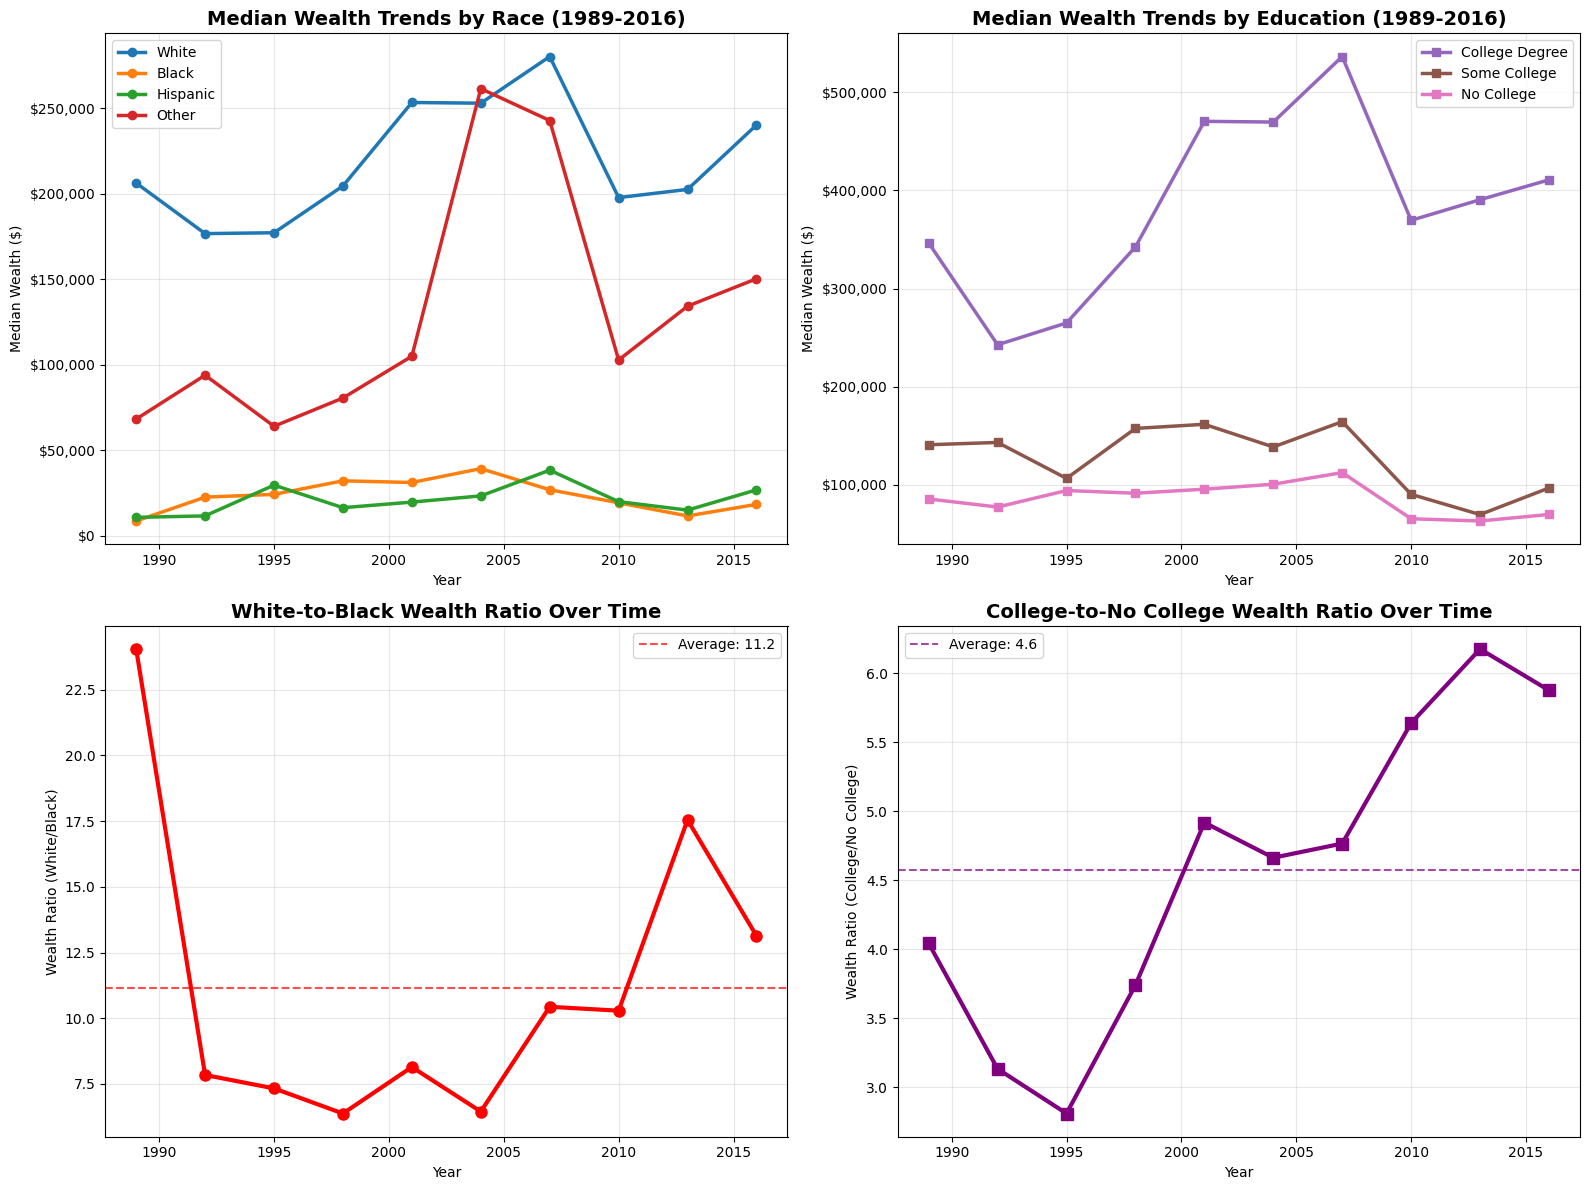
\includegraphics{main_files/figure-pdf/cell-10-output-1.png}

\begin{Shaded}
\begin{Highlighting}[]
\CommentTok{\# Create heatmap showing wealth by race and education over time}
\NormalTok{fig, (ax1, ax2) }\OperatorTok{=}\NormalTok{ plt.subplots(}\DecValTok{1}\NormalTok{, }\DecValTok{2}\NormalTok{, figsize}\OperatorTok{=}\NormalTok{(}\DecValTok{18}\NormalTok{, }\DecValTok{6}\NormalTok{))}

\CommentTok{\# Prepare data for heatmap {-} Average wealth by race and education}
\NormalTok{heatmap\_data }\OperatorTok{=}\NormalTok{ []}
\ControlFlowTok{for}\NormalTok{ race }\KeywordTok{in}\NormalTok{ df[}\StringTok{\textquotesingle{}race\textquotesingle{}}\NormalTok{].unique():}
    \ControlFlowTok{for}\NormalTok{ education }\KeywordTok{in}\NormalTok{ df[}\StringTok{\textquotesingle{}education\textquotesingle{}}\NormalTok{].unique():}
\NormalTok{        subset }\OperatorTok{=}\NormalTok{ df[(df[}\StringTok{\textquotesingle{}race\textquotesingle{}}\NormalTok{] }\OperatorTok{==}\NormalTok{ race) }\OperatorTok{\&}\NormalTok{ (df[}\StringTok{\textquotesingle{}education\textquotesingle{}}\NormalTok{] }\OperatorTok{==}\NormalTok{ education)]}
        \ControlFlowTok{if} \BuiltInTok{len}\NormalTok{(subset) }\OperatorTok{\textgreater{}} \DecValTok{0}\NormalTok{:}
\NormalTok{            weighted\_med }\OperatorTok{=}\NormalTok{ weighted\_median(subset[}\StringTok{\textquotesingle{}wealth\textquotesingle{}}\NormalTok{].values, subset[}\StringTok{\textquotesingle{}weight\textquotesingle{}}\NormalTok{].values)}
\NormalTok{            heatmap\_data.append(\{}
                \StringTok{\textquotesingle{}race\textquotesingle{}}\NormalTok{: race,}
                \StringTok{\textquotesingle{}education\textquotesingle{}}\NormalTok{: education,}
                \StringTok{\textquotesingle{}weighted\_median\_wealth\textquotesingle{}}\NormalTok{: weighted\_med}
\NormalTok{            \})}

\NormalTok{heatmap\_df }\OperatorTok{=}\NormalTok{ pd.DataFrame(heatmap\_data)}
\NormalTok{heatmap\_pivot }\OperatorTok{=}\NormalTok{ heatmap\_df.pivot(index}\OperatorTok{=}\StringTok{\textquotesingle{}race\textquotesingle{}}\NormalTok{, columns}\OperatorTok{=}\StringTok{\textquotesingle{}education\textquotesingle{}}\NormalTok{, values}\OperatorTok{=}\StringTok{\textquotesingle{}weighted\_median\_wealth\textquotesingle{}}\NormalTok{)}

\CommentTok{\# Heatmap 1: Overall wealth by race and education}
\NormalTok{sns.heatmap(heatmap\_pivot, annot}\OperatorTok{=}\VariableTok{True}\NormalTok{, fmt}\OperatorTok{=}\StringTok{\textquotesingle{}.0f\textquotesingle{}}\NormalTok{, cmap}\OperatorTok{=}\StringTok{\textquotesingle{}YlOrRd\textquotesingle{}}\NormalTok{, ax}\OperatorTok{=}\NormalTok{ax1, }
\NormalTok{            cbar\_kws}\OperatorTok{=}\NormalTok{\{}\StringTok{\textquotesingle{}label\textquotesingle{}}\NormalTok{: }\StringTok{\textquotesingle{}Median Wealth ($)\textquotesingle{}}\NormalTok{\})}
\NormalTok{ax1.set\_title(}\StringTok{\textquotesingle{}Overall Median Wealth by Race and Education}\CharTok{\textbackslash{}n}\StringTok{(1989{-}2016 Average)\textquotesingle{}}\NormalTok{, }
\NormalTok{              fontsize}\OperatorTok{=}\DecValTok{14}\NormalTok{, fontweight}\OperatorTok{=}\StringTok{\textquotesingle{}bold\textquotesingle{}}\NormalTok{)}
\NormalTok{ax1.set\_ylabel(}\StringTok{\textquotesingle{}Race\textquotesingle{}}\NormalTok{)}
\NormalTok{ax1.set\_xlabel(}\StringTok{\textquotesingle{}Education Level\textquotesingle{}}\NormalTok{)}

\CommentTok{\# Create wealth change comparison (2016 vs 1989)}
\NormalTok{early\_data }\OperatorTok{=}\NormalTok{ df[df[}\StringTok{\textquotesingle{}year\textquotesingle{}}\NormalTok{] }\OperatorTok{==} \DecValTok{1989}\NormalTok{]}
\NormalTok{recent\_data }\OperatorTok{=}\NormalTok{ df[df[}\StringTok{\textquotesingle{}year\textquotesingle{}}\NormalTok{] }\OperatorTok{==} \DecValTok{2016}\NormalTok{]}

\NormalTok{change\_data }\OperatorTok{=}\NormalTok{ []}
\ControlFlowTok{for}\NormalTok{ race }\KeywordTok{in}\NormalTok{ df[}\StringTok{\textquotesingle{}race\textquotesingle{}}\NormalTok{].unique():}
    \ControlFlowTok{for}\NormalTok{ education }\KeywordTok{in}\NormalTok{ df[}\StringTok{\textquotesingle{}education\textquotesingle{}}\NormalTok{].unique():}
\NormalTok{        early\_subset }\OperatorTok{=}\NormalTok{ early\_data[(early\_data[}\StringTok{\textquotesingle{}race\textquotesingle{}}\NormalTok{] }\OperatorTok{==}\NormalTok{ race) }\OperatorTok{\&}\NormalTok{ (early\_data[}\StringTok{\textquotesingle{}education\textquotesingle{}}\NormalTok{] }\OperatorTok{==}\NormalTok{ education)]}
\NormalTok{        recent\_subset }\OperatorTok{=}\NormalTok{ recent\_data[(recent\_data[}\StringTok{\textquotesingle{}race\textquotesingle{}}\NormalTok{] }\OperatorTok{==}\NormalTok{ race) }\OperatorTok{\&}\NormalTok{ (recent\_data[}\StringTok{\textquotesingle{}education\textquotesingle{}}\NormalTok{] }\OperatorTok{==}\NormalTok{ education)]}
        
        \ControlFlowTok{if} \BuiltInTok{len}\NormalTok{(early\_subset) }\OperatorTok{\textgreater{}} \DecValTok{0} \KeywordTok{and} \BuiltInTok{len}\NormalTok{(recent\_subset) }\OperatorTok{\textgreater{}} \DecValTok{0}\NormalTok{:}
\NormalTok{            early\_wealth }\OperatorTok{=}\NormalTok{ weighted\_median(early\_subset[}\StringTok{\textquotesingle{}wealth\textquotesingle{}}\NormalTok{].values, early\_subset[}\StringTok{\textquotesingle{}weight\textquotesingle{}}\NormalTok{].values)}
\NormalTok{            recent\_wealth }\OperatorTok{=}\NormalTok{ weighted\_median(recent\_subset[}\StringTok{\textquotesingle{}wealth\textquotesingle{}}\NormalTok{].values, recent\_subset[}\StringTok{\textquotesingle{}weight\textquotesingle{}}\NormalTok{].values)}
            
            \ControlFlowTok{if} \KeywordTok{not}\NormalTok{ np.isnan(early\_wealth) }\KeywordTok{and} \KeywordTok{not}\NormalTok{ np.isnan(recent\_wealth):}
\NormalTok{                pct\_change }\OperatorTok{=}\NormalTok{ ((recent\_wealth }\OperatorTok{{-}}\NormalTok{ early\_wealth) }\OperatorTok{/}\NormalTok{ early\_wealth) }\OperatorTok{*} \DecValTok{100}
\NormalTok{                change\_data.append(\{}
                    \StringTok{\textquotesingle{}race\textquotesingle{}}\NormalTok{: race,}
                    \StringTok{\textquotesingle{}education\textquotesingle{}}\NormalTok{: education,}
                    \StringTok{\textquotesingle{}percent\_change\textquotesingle{}}\NormalTok{: pct\_change}
\NormalTok{                \})}

\NormalTok{change\_df }\OperatorTok{=}\NormalTok{ pd.DataFrame(change\_data)}
\NormalTok{change\_pivot }\OperatorTok{=}\NormalTok{ change\_df.pivot(index}\OperatorTok{=}\StringTok{\textquotesingle{}race\textquotesingle{}}\NormalTok{, columns}\OperatorTok{=}\StringTok{\textquotesingle{}education\textquotesingle{}}\NormalTok{, values}\OperatorTok{=}\StringTok{\textquotesingle{}percent\_change\textquotesingle{}}\NormalTok{)}

\CommentTok{\# Heatmap 2: Percentage change in wealth (2016 vs 1989)}
\NormalTok{sns.heatmap(change\_pivot, annot}\OperatorTok{=}\VariableTok{True}\NormalTok{, fmt}\OperatorTok{=}\StringTok{\textquotesingle{}.1f\textquotesingle{}}\NormalTok{, cmap}\OperatorTok{=}\StringTok{\textquotesingle{}RdBu\_r\textquotesingle{}}\NormalTok{, center}\OperatorTok{=}\DecValTok{0}\NormalTok{, ax}\OperatorTok{=}\NormalTok{ax2,}
\NormalTok{            cbar\_kws}\OperatorTok{=}\NormalTok{\{}\StringTok{\textquotesingle{}label\textquotesingle{}}\NormalTok{: }\StringTok{\textquotesingle{}Percent Change (\%)\textquotesingle{}}\NormalTok{\})}
\NormalTok{ax2.set\_title(}\StringTok{\textquotesingle{}Wealth Change: 2016 vs 1989}\CharTok{\textbackslash{}n}\StringTok{(Percentage Change)\textquotesingle{}}\NormalTok{, }
\NormalTok{              fontsize}\OperatorTok{=}\DecValTok{14}\NormalTok{, fontweight}\OperatorTok{=}\StringTok{\textquotesingle{}bold\textquotesingle{}}\NormalTok{)}
\NormalTok{ax2.set\_ylabel(}\StringTok{\textquotesingle{}Race\textquotesingle{}}\NormalTok{)}
\NormalTok{ax2.set\_xlabel(}\StringTok{\textquotesingle{}Education Level\textquotesingle{}}\NormalTok{)}

\NormalTok{plt.tight\_layout()}
\NormalTok{plt.show()}
\end{Highlighting}
\end{Shaded}

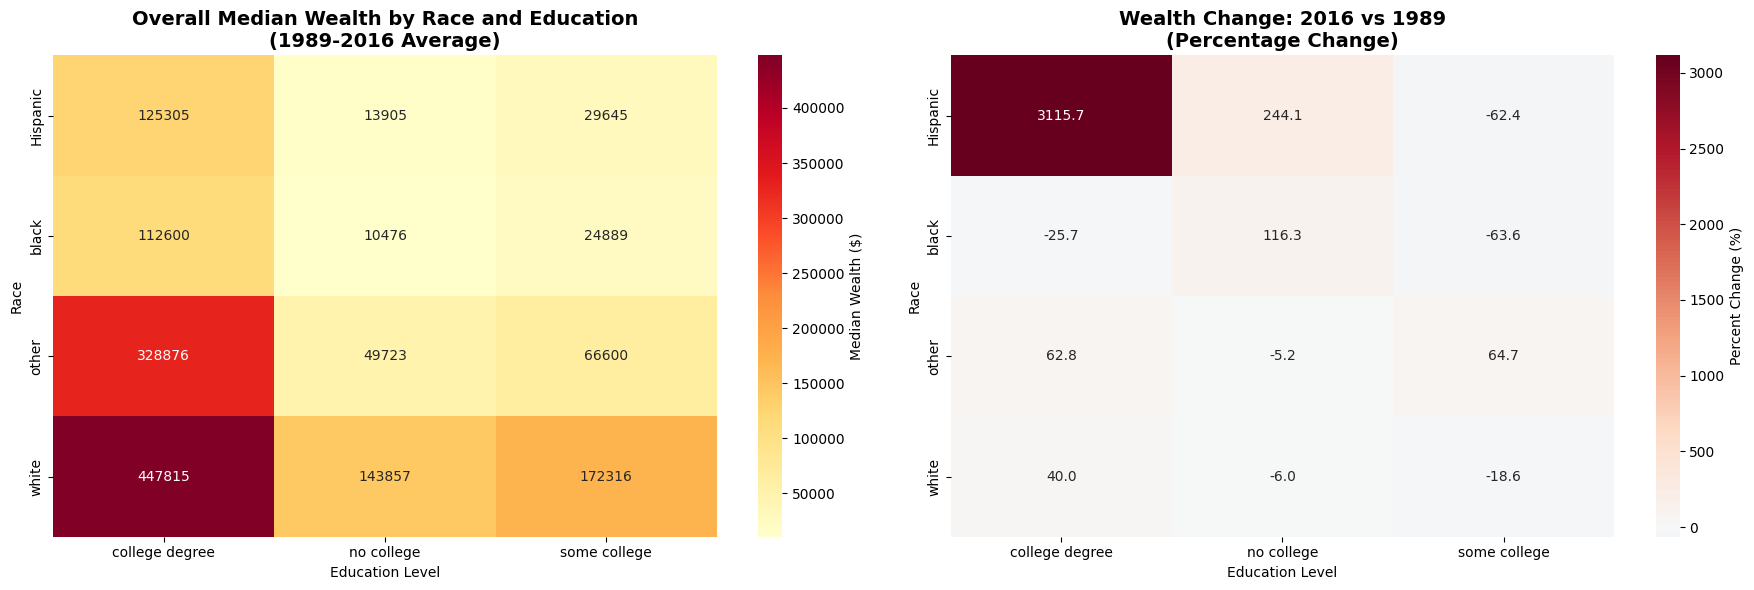
\includegraphics{main_files/figure-pdf/cell-11-output-1.png}

\begin{Shaded}
\begin{Highlighting}[]
\CommentTok{\# Quantitative Analysis of Trends}
\BuiltInTok{print}\NormalTok{(}\StringTok{"=== QUANTITATIVE TREND ANALYSIS ===}\CharTok{\textbackslash{}n}\StringTok{"}\NormalTok{)}

\CommentTok{\# Calculate compound annual growth rates (CAGR) for each group}
\KeywordTok{def}\NormalTok{ calculate\_cagr(start\_value, end\_value, years):}
    \ControlFlowTok{if}\NormalTok{ start\_value }\OperatorTok{\textless{}=} \DecValTok{0} \KeywordTok{or}\NormalTok{ end\_value }\OperatorTok{\textless{}=} \DecValTok{0}\NormalTok{:}
        \ControlFlowTok{return}\NormalTok{ np.nan}
    \ControlFlowTok{return}\NormalTok{ ((end\_value }\OperatorTok{/}\NormalTok{ start\_value) }\OperatorTok{**}\NormalTok{ (}\DecValTok{1}\OperatorTok{/}\NormalTok{years) }\OperatorTok{{-}} \DecValTok{1}\NormalTok{) }\OperatorTok{*} \DecValTok{100}

\NormalTok{years\_span }\OperatorTok{=} \DecValTok{2016} \OperatorTok{{-}} \DecValTok{1989}

\BuiltInTok{print}\NormalTok{(}\StringTok{"1. COMPOUND ANNUAL GROWTH RATES (1989{-}2016):"}\NormalTok{)}
\BuiltInTok{print}\NormalTok{(}\StringTok{"   Race Groups:"}\NormalTok{)}
\ControlFlowTok{for}\NormalTok{ race }\KeywordTok{in}\NormalTok{ [}\StringTok{\textquotesingle{}white\textquotesingle{}}\NormalTok{, }\StringTok{\textquotesingle{}black\textquotesingle{}}\NormalTok{, }\StringTok{\textquotesingle{}Hispanic\textquotesingle{}}\NormalTok{, }\StringTok{\textquotesingle{}other\textquotesingle{}}\NormalTok{]:}
\NormalTok{    start\_val }\OperatorTok{=}\NormalTok{ pivot\_race.loc[}\DecValTok{1989}\NormalTok{, race] }\ControlFlowTok{if}\NormalTok{ race }\KeywordTok{in}\NormalTok{ pivot\_race.columns }\ControlFlowTok{else}\NormalTok{ np.nan}
\NormalTok{    end\_val }\OperatorTok{=}\NormalTok{ pivot\_race.loc[}\DecValTok{2016}\NormalTok{, race] }\ControlFlowTok{if}\NormalTok{ race }\KeywordTok{in}\NormalTok{ pivot\_race.columns }\ControlFlowTok{else}\NormalTok{ np.nan}
\NormalTok{    cagr }\OperatorTok{=}\NormalTok{ calculate\_cagr(start\_val, end\_val, years\_span)}
    \BuiltInTok{print}\NormalTok{(}\SpecialStringTok{f"   {-} }\SpecialCharTok{\{}\NormalTok{race}\SpecialCharTok{.}\NormalTok{title()}\SpecialCharTok{\}}\SpecialStringTok{: }\SpecialCharTok{\{}\NormalTok{cagr}\SpecialCharTok{:.2f\}}\SpecialStringTok{\% per year"}\NormalTok{)}

\BuiltInTok{print}\NormalTok{(}\StringTok{"}\CharTok{\textbackslash{}n}\StringTok{   Education Groups:"}\NormalTok{)}
\ControlFlowTok{for}\NormalTok{ edu }\KeywordTok{in}\NormalTok{ [}\StringTok{\textquotesingle{}college degree\textquotesingle{}}\NormalTok{, }\StringTok{\textquotesingle{}some college\textquotesingle{}}\NormalTok{, }\StringTok{\textquotesingle{}no college\textquotesingle{}}\NormalTok{]:}
\NormalTok{    start\_val }\OperatorTok{=}\NormalTok{ pivot\_edu.loc[}\DecValTok{1989}\NormalTok{, edu] }\ControlFlowTok{if}\NormalTok{ edu }\KeywordTok{in}\NormalTok{ pivot\_edu.columns }\ControlFlowTok{else}\NormalTok{ np.nan}
\NormalTok{    end\_val }\OperatorTok{=}\NormalTok{ pivot\_edu.loc[}\DecValTok{2016}\NormalTok{, edu] }\ControlFlowTok{if}\NormalTok{ edu }\KeywordTok{in}\NormalTok{ pivot\_edu.columns }\ControlFlowTok{else}\NormalTok{ np.nan}
\NormalTok{    cagr }\OperatorTok{=}\NormalTok{ calculate\_cagr(start\_val, end\_val, years\_span)}
    \BuiltInTok{print}\NormalTok{(}\SpecialStringTok{f"   {-} }\SpecialCharTok{\{}\NormalTok{edu}\SpecialCharTok{.}\NormalTok{title()}\SpecialCharTok{\}}\SpecialStringTok{: }\SpecialCharTok{\{}\NormalTok{cagr}\SpecialCharTok{:.2f\}}\SpecialStringTok{\% per year"}\NormalTok{)}

\CommentTok{\# Gap analysis}
\BuiltInTok{print}\NormalTok{(}\StringTok{"}\CharTok{\textbackslash{}n}\StringTok{2. WEALTH GAP ANALYSIS:"}\NormalTok{)}
\NormalTok{white\_black\_1989 }\OperatorTok{=}\NormalTok{ pivot\_race.loc[}\DecValTok{1989}\NormalTok{, }\StringTok{\textquotesingle{}white\textquotesingle{}}\NormalTok{] }\OperatorTok{/}\NormalTok{ pivot\_race.loc[}\DecValTok{1989}\NormalTok{, }\StringTok{\textquotesingle{}black\textquotesingle{}}\NormalTok{]}
\NormalTok{white\_black\_2016 }\OperatorTok{=}\NormalTok{ pivot\_race.loc[}\DecValTok{2016}\NormalTok{, }\StringTok{\textquotesingle{}white\textquotesingle{}}\NormalTok{] }\OperatorTok{/}\NormalTok{ pivot\_race.loc[}\DecValTok{2016}\NormalTok{, }\StringTok{\textquotesingle{}black\textquotesingle{}}\NormalTok{]}
\BuiltInTok{print}\NormalTok{(}\SpecialStringTok{f"   White{-}to{-}Black Ratio: }\SpecialCharTok{\{}\NormalTok{white\_black\_1989}\SpecialCharTok{:.1f\}}\SpecialStringTok{ (1989) → }\SpecialCharTok{\{}\NormalTok{white\_black\_2016}\SpecialCharTok{:.1f\}}\SpecialStringTok{ (2016)"}\NormalTok{)}

\NormalTok{college\_no\_college\_1989 }\OperatorTok{=}\NormalTok{ pivot\_edu.loc[}\DecValTok{1989}\NormalTok{, }\StringTok{\textquotesingle{}college degree\textquotesingle{}}\NormalTok{] }\OperatorTok{/}\NormalTok{ pivot\_edu.loc[}\DecValTok{1989}\NormalTok{, }\StringTok{\textquotesingle{}no college\textquotesingle{}}\NormalTok{]}
\NormalTok{college\_no\_college\_2016 }\OperatorTok{=}\NormalTok{ pivot\_edu.loc[}\DecValTok{2016}\NormalTok{, }\StringTok{\textquotesingle{}college degree\textquotesingle{}}\NormalTok{] }\OperatorTok{/}\NormalTok{ pivot\_edu.loc[}\DecValTok{2016}\NormalTok{, }\StringTok{\textquotesingle{}no college\textquotesingle{}}\NormalTok{]}
\BuiltInTok{print}\NormalTok{(}\SpecialStringTok{f"   College{-}to{-}No College Ratio: }\SpecialCharTok{\{}\NormalTok{college\_no\_college\_1989}\SpecialCharTok{:.1f\}}\SpecialStringTok{ (1989) → }\SpecialCharTok{\{}\NormalTok{college\_no\_college\_2016}\SpecialCharTok{:.1f\}}\SpecialStringTok{ (2016)"}\NormalTok{)}

\CommentTok{\# Volatility analysis (coefficient of variation)}
\BuiltInTok{print}\NormalTok{(}\StringTok{"}\CharTok{\textbackslash{}n}\StringTok{3. WEALTH VOLATILITY (Coefficient of Variation):"}\NormalTok{)}
\BuiltInTok{print}\NormalTok{(}\StringTok{"   Race Groups:"}\NormalTok{)}
\ControlFlowTok{for}\NormalTok{ race }\KeywordTok{in}\NormalTok{ [}\StringTok{\textquotesingle{}white\textquotesingle{}}\NormalTok{, }\StringTok{\textquotesingle{}black\textquotesingle{}}\NormalTok{, }\StringTok{\textquotesingle{}Hispanic\textquotesingle{}}\NormalTok{, }\StringTok{\textquotesingle{}other\textquotesingle{}}\NormalTok{]:}
    \ControlFlowTok{if}\NormalTok{ race }\KeywordTok{in}\NormalTok{ pivot\_race.columns:}
\NormalTok{        cv }\OperatorTok{=}\NormalTok{ (pivot\_race[race].std() }\OperatorTok{/}\NormalTok{ pivot\_race[race].mean()) }\OperatorTok{*} \DecValTok{100}
        \BuiltInTok{print}\NormalTok{(}\SpecialStringTok{f"   {-} }\SpecialCharTok{\{}\NormalTok{race}\SpecialCharTok{.}\NormalTok{title()}\SpecialCharTok{\}}\SpecialStringTok{: }\SpecialCharTok{\{}\NormalTok{cv}\SpecialCharTok{:.1f\}}\SpecialStringTok{\%"}\NormalTok{)}

\BuiltInTok{print}\NormalTok{(}\StringTok{"}\CharTok{\textbackslash{}n}\StringTok{   Education Groups:"}\NormalTok{)}
\ControlFlowTok{for}\NormalTok{ edu }\KeywordTok{in}\NormalTok{ [}\StringTok{\textquotesingle{}college degree\textquotesingle{}}\NormalTok{, }\StringTok{\textquotesingle{}some college\textquotesingle{}}\NormalTok{, }\StringTok{\textquotesingle{}no college\textquotesingle{}}\NormalTok{]:}
    \ControlFlowTok{if}\NormalTok{ edu }\KeywordTok{in}\NormalTok{ pivot\_edu.columns:}
\NormalTok{        cv }\OperatorTok{=}\NormalTok{ (pivot\_edu[edu].std() }\OperatorTok{/}\NormalTok{ pivot\_edu[edu].mean()) }\OperatorTok{*} \DecValTok{100}
        \BuiltInTok{print}\NormalTok{(}\SpecialStringTok{f"   {-} }\SpecialCharTok{\{}\NormalTok{edu}\SpecialCharTok{.}\NormalTok{title()}\SpecialCharTok{\}}\SpecialStringTok{: }\SpecialCharTok{\{}\NormalTok{cv}\SpecialCharTok{:.1f\}}\SpecialStringTok{\%"}\NormalTok{)}

\CommentTok{\# Crisis impact analysis (2007{-}2010)}
\BuiltInTok{print}\NormalTok{(}\StringTok{"}\CharTok{\textbackslash{}n}\StringTok{4. FINANCIAL CRISIS IMPACT (2007{-}2010):"}\NormalTok{)}
\BuiltInTok{print}\NormalTok{(}\StringTok{"   Race Groups:"}\NormalTok{)}
\ControlFlowTok{for}\NormalTok{ race }\KeywordTok{in}\NormalTok{ [}\StringTok{\textquotesingle{}white\textquotesingle{}}\NormalTok{, }\StringTok{\textquotesingle{}black\textquotesingle{}}\NormalTok{, }\StringTok{\textquotesingle{}Hispanic\textquotesingle{}}\NormalTok{, }\StringTok{\textquotesingle{}other\textquotesingle{}}\NormalTok{]:}
    \ControlFlowTok{if}\NormalTok{ race }\KeywordTok{in}\NormalTok{ pivot\_race.columns:}
\NormalTok{        crisis\_decline }\OperatorTok{=}\NormalTok{ ((pivot\_race.loc[}\DecValTok{2010}\NormalTok{, race] }\OperatorTok{{-}}\NormalTok{ pivot\_race.loc[}\DecValTok{2007}\NormalTok{, race]) }\OperatorTok{/}\NormalTok{ pivot\_race.loc[}\DecValTok{2007}\NormalTok{, race]) }\OperatorTok{*} \DecValTok{100}
        \BuiltInTok{print}\NormalTok{(}\SpecialStringTok{f"   {-} }\SpecialCharTok{\{}\NormalTok{race}\SpecialCharTok{.}\NormalTok{title()}\SpecialCharTok{\}}\SpecialStringTok{: }\SpecialCharTok{\{}\NormalTok{crisis\_decline}\SpecialCharTok{:.1f\}}\SpecialStringTok{\%"}\NormalTok{)}

\BuiltInTok{print}\NormalTok{(}\StringTok{"}\CharTok{\textbackslash{}n}\StringTok{   Education Groups:"}\NormalTok{)}
\ControlFlowTok{for}\NormalTok{ edu }\KeywordTok{in}\NormalTok{ [}\StringTok{\textquotesingle{}college degree\textquotesingle{}}\NormalTok{, }\StringTok{\textquotesingle{}some college\textquotesingle{}}\NormalTok{, }\StringTok{\textquotesingle{}no college\textquotesingle{}}\NormalTok{]:}
    \ControlFlowTok{if}\NormalTok{ edu }\KeywordTok{in}\NormalTok{ pivot\_edu.columns:}
\NormalTok{        crisis\_decline }\OperatorTok{=}\NormalTok{ ((pivot\_edu.loc[}\DecValTok{2010}\NormalTok{, edu] }\OperatorTok{{-}}\NormalTok{ pivot\_edu.loc[}\DecValTok{2007}\NormalTok{, edu]) }\OperatorTok{/}\NormalTok{ pivot\_edu.loc[}\DecValTok{2007}\NormalTok{, edu]) }\OperatorTok{*} \DecValTok{100}
        \BuiltInTok{print}\NormalTok{(}\SpecialStringTok{f"   {-} }\SpecialCharTok{\{}\NormalTok{edu}\SpecialCharTok{.}\NormalTok{title()}\SpecialCharTok{\}}\SpecialStringTok{: }\SpecialCharTok{\{}\NormalTok{crisis\_decline}\SpecialCharTok{:.1f\}}\SpecialStringTok{\%"}\NormalTok{)}

\BuiltInTok{print}\NormalTok{(}\StringTok{"}\CharTok{\textbackslash{}n}\StringTok{=== END ANALYSIS ==="}\NormalTok{)  }
\end{Highlighting}
\end{Shaded}

\begin{verbatim}
=== QUANTITATIVE TREND ANALYSIS ===

1. COMPOUND ANNUAL GROWTH RATES (1989-2016):
   Race Groups:
   - White: 0.57% per year
   - Black: 2.84% per year
   - Hispanic: 3.46% per year
   - Other: 2.97% per year

   Education Groups:
   - College Degree: 0.63% per year
   - Some College: -1.38% per year
   - No College: -0.75% per year

2. WEALTH GAP ANALYSIS:
   White-to-Black Ratio: 24.0 (1989) → 13.1 (2016)
   College-to-No College Ratio: 4.0 (1989) → 5.9 (2016)

3. WEALTH VOLATILITY (Coefficient of Variation):
   Race Groups:
   - White: 16.1%
   - Black: 40.4%
   - Hispanic: 40.8%
   - Other: 53.5%

   Education Groups:
   - College Degree: 23.9%
   - Some College: 26.3%
   - No College: 19.0%

4. FINANCIAL CRISIS IMPACT (2007-2010):
   Race Groups:
   - White: -29.4%
   - Black: -28.4%
   - Hispanic: -48.1%
   - Other: -57.7%

   Education Groups:
   - College Degree: -31.1%
   - Some College: -45.0%
   - No College: -41.8%

=== END ANALYSIS ===
\end{verbatim}

This section focuses specifically on median housing wealth trends for
Black and White households, using weighted medians to ensure
population-representative results.

\begin{Shaded}
\begin{Highlighting}[]
\CommentTok{\# Calculate weighted median housing wealth by race and year (Black and White only)}
\NormalTok{housing\_wealth\_by\_race }\OperatorTok{=}\NormalTok{ []}

\CommentTok{\# Focus on Black and White households only}
\NormalTok{target\_races }\OperatorTok{=}\NormalTok{ [}\StringTok{\textquotesingle{}black\textquotesingle{}}\NormalTok{, }\StringTok{\textquotesingle{}white\textquotesingle{}}\NormalTok{]}

\ControlFlowTok{for}\NormalTok{ year }\KeywordTok{in} \BuiltInTok{sorted}\NormalTok{(df[}\StringTok{\textquotesingle{}year\textquotesingle{}}\NormalTok{].unique()):}
    \ControlFlowTok{for}\NormalTok{ race }\KeywordTok{in}\NormalTok{ target\_races:}
\NormalTok{        subset }\OperatorTok{=}\NormalTok{ df[(df[}\StringTok{\textquotesingle{}year\textquotesingle{}}\NormalTok{] }\OperatorTok{==}\NormalTok{ year) }\OperatorTok{\&}\NormalTok{ (df[}\StringTok{\textquotesingle{}race\textquotesingle{}}\NormalTok{] }\OperatorTok{==}\NormalTok{ race)]}
        \ControlFlowTok{if} \BuiltInTok{len}\NormalTok{(subset) }\OperatorTok{\textgreater{}} \DecValTok{0}\NormalTok{:}
            \CommentTok{\# Use asset\_housing for housing wealth}
\NormalTok{            weighted\_med\_housing }\OperatorTok{=}\NormalTok{ weighted\_median(subset[}\StringTok{\textquotesingle{}asset\_housing\textquotesingle{}}\NormalTok{].values, subset[}\StringTok{\textquotesingle{}weight\textquotesingle{}}\NormalTok{].values)}
\NormalTok{            housing\_wealth\_by\_race.append(\{}
                \StringTok{\textquotesingle{}year\textquotesingle{}}\NormalTok{: year,}
                \StringTok{\textquotesingle{}race\textquotesingle{}}\NormalTok{: race,}
                \StringTok{\textquotesingle{}weighted\_median\_housing\_wealth\textquotesingle{}}\NormalTok{: weighted\_med\_housing,}
                \StringTok{\textquotesingle{}sample\_size\textquotesingle{}}\NormalTok{: }\BuiltInTok{len}\NormalTok{(subset)}
\NormalTok{            \})}

\NormalTok{housing\_wealth\_df }\OperatorTok{=}\NormalTok{ pd.DataFrame(housing\_wealth\_by\_race)}
\NormalTok{housing\_pivot }\OperatorTok{=}\NormalTok{ housing\_wealth\_df.pivot(index}\OperatorTok{=}\StringTok{\textquotesingle{}year\textquotesingle{}}\NormalTok{, columns}\OperatorTok{=}\StringTok{\textquotesingle{}race\textquotesingle{}}\NormalTok{, values}\OperatorTok{=}\StringTok{\textquotesingle{}weighted\_median\_housing\_wealth\textquotesingle{}}\NormalTok{)}

\BuiltInTok{print}\NormalTok{(}\StringTok{"Weighted median housing wealth by race and year (Black vs White):"}\NormalTok{)}
\BuiltInTok{print}\NormalTok{(housing\_pivot.}\BuiltInTok{round}\NormalTok{(}\DecValTok{0}\NormalTok{))}
\BuiltInTok{print}\NormalTok{(}\SpecialStringTok{f"}\CharTok{\textbackslash{}n}\SpecialStringTok{Data covers }\SpecialCharTok{\{}\BuiltInTok{len}\NormalTok{(df)}\SpecialCharTok{\}}\SpecialStringTok{ total observations from }\SpecialCharTok{\{}\NormalTok{df[}\StringTok{\textquotesingle{}year\textquotesingle{}}\NormalTok{]}\SpecialCharTok{.}\BuiltInTok{min}\NormalTok{()}\SpecialCharTok{\}}\SpecialStringTok{ to }\SpecialCharTok{\{}\NormalTok{df[}\StringTok{\textquotesingle{}year\textquotesingle{}}\NormalTok{]}\SpecialCharTok{.}\BuiltInTok{max}\NormalTok{()}\SpecialCharTok{\}}\SpecialStringTok{"}\NormalTok{)}
\BuiltInTok{print}\NormalTok{(}\SpecialStringTok{f"Analysis focuses on }\SpecialCharTok{\{}\BuiltInTok{len}\NormalTok{(df[df[}\StringTok{\textquotesingle{}race\textquotesingle{}}\NormalTok{].isin(target\_races)])}\SpecialCharTok{\}}\SpecialStringTok{ Black and White households"}\NormalTok{)}
\end{Highlighting}
\end{Shaded}

\begin{verbatim}
Weighted median housing wealth by race and year (Black vs White):
race   black     white
year                  
1989     0.0   93293.0
1992     0.0   92239.0
1995     0.0  101790.0
1998     0.0  115086.0
2001     0.0  121937.0
2004  7631.0  158973.0
2007     0.0  162122.0
2010     0.0  138166.0
2013     0.0  128888.0
2016     0.0  130000.0

Data covers 47776 total observations from 1989 to 2016
Analysis focuses on 42230 Black and White households
\end{verbatim}

\begin{Shaded}
\begin{Highlighting}[]
\CommentTok{\# Create comprehensive visualizations for housing wealth}
\NormalTok{fig, ((ax1, ax2), (ax3, ax4)) }\OperatorTok{=}\NormalTok{ plt.subplots(}\DecValTok{2}\NormalTok{, }\DecValTok{2}\NormalTok{, figsize}\OperatorTok{=}\NormalTok{(}\DecValTok{16}\NormalTok{, }\DecValTok{12}\NormalTok{))}

\CommentTok{\# Plot 1: Housing wealth trends by race}
\NormalTok{colors\_race }\OperatorTok{=}\NormalTok{ [}\StringTok{\textquotesingle{}\#1f77b4\textquotesingle{}}\NormalTok{, }\StringTok{\textquotesingle{}\#ff7f0e\textquotesingle{}}\NormalTok{]  }\CommentTok{\# Blue for White, Orange for Black}
\ControlFlowTok{for}\NormalTok{ i, race }\KeywordTok{in} \BuiltInTok{enumerate}\NormalTok{([}\StringTok{\textquotesingle{}white\textquotesingle{}}\NormalTok{, }\StringTok{\textquotesingle{}black\textquotesingle{}}\NormalTok{]):}
    \ControlFlowTok{if}\NormalTok{ race }\KeywordTok{in}\NormalTok{ housing\_pivot.columns:}
\NormalTok{        ax1.plot(housing\_pivot.index, housing\_pivot[race], marker}\OperatorTok{=}\StringTok{\textquotesingle{}o\textquotesingle{}}\NormalTok{, linewidth}\OperatorTok{=}\DecValTok{3}\NormalTok{, }
\NormalTok{                label}\OperatorTok{=}\SpecialStringTok{f\textquotesingle{}}\SpecialCharTok{\{}\NormalTok{race}\SpecialCharTok{.}\NormalTok{title()}\SpecialCharTok{\}}\SpecialStringTok{ Households\textquotesingle{}}\NormalTok{, color}\OperatorTok{=}\NormalTok{colors\_race[i], markersize}\OperatorTok{=}\DecValTok{8}\NormalTok{)}

\NormalTok{ax1.set\_title(}\StringTok{\textquotesingle{}Median Housing Wealth Trends: Black vs White Households}\CharTok{\textbackslash{}n}\StringTok{(1989{-}2016)\textquotesingle{}}\NormalTok{, }
\NormalTok{              fontsize}\OperatorTok{=}\DecValTok{14}\NormalTok{, fontweight}\OperatorTok{=}\StringTok{\textquotesingle{}bold\textquotesingle{}}\NormalTok{)}
\NormalTok{ax1.set\_xlabel(}\StringTok{\textquotesingle{}Year\textquotesingle{}}\NormalTok{)}
\NormalTok{ax1.set\_ylabel(}\StringTok{\textquotesingle{}Median Housing Wealth ($)\textquotesingle{}}\NormalTok{)}
\NormalTok{ax1.legend()}
\NormalTok{ax1.grid(}\VariableTok{True}\NormalTok{, alpha}\OperatorTok{=}\FloatTok{0.3}\NormalTok{)}
\NormalTok{ax1.yaxis.set\_major\_formatter(plt.FuncFormatter(}\KeywordTok{lambda}\NormalTok{ x, p: }\SpecialStringTok{f\textquotesingle{}$}\SpecialCharTok{\{}\NormalTok{x}\SpecialCharTok{:,.0f\}}\SpecialStringTok{\textquotesingle{}}\NormalTok{))}

\CommentTok{\# Plot 2: Housing wealth gap (absolute difference)}
\NormalTok{white\_housing }\OperatorTok{=}\NormalTok{ housing\_pivot[}\StringTok{\textquotesingle{}white\textquotesingle{}}\NormalTok{]}
\NormalTok{black\_housing }\OperatorTok{=}\NormalTok{ housing\_pivot[}\StringTok{\textquotesingle{}black\textquotesingle{}}\NormalTok{]}
\NormalTok{housing\_gap }\OperatorTok{=}\NormalTok{ white\_housing }\OperatorTok{{-}}\NormalTok{ black\_housing}

\NormalTok{ax2.fill\_between(housing\_gap.index, }\DecValTok{0}\NormalTok{, housing\_gap.values, alpha}\OperatorTok{=}\FloatTok{0.6}\NormalTok{, color}\OperatorTok{=}\StringTok{\textquotesingle{}red\textquotesingle{}}\NormalTok{)}
\NormalTok{ax2.plot(housing\_gap.index, housing\_gap.values, marker}\OperatorTok{=}\StringTok{\textquotesingle{}s\textquotesingle{}}\NormalTok{, linewidth}\OperatorTok{=}\DecValTok{2}\NormalTok{, }
\NormalTok{         color}\OperatorTok{=}\StringTok{\textquotesingle{}darkred\textquotesingle{}}\NormalTok{, markersize}\OperatorTok{=}\DecValTok{6}\NormalTok{)}
\NormalTok{ax2.set\_title(}\StringTok{\textquotesingle{}Housing Wealth Gap (White {-} Black)}\CharTok{\textbackslash{}n}\StringTok{Absolute Difference\textquotesingle{}}\NormalTok{, }
\NormalTok{              fontsize}\OperatorTok{=}\DecValTok{14}\NormalTok{, fontweight}\OperatorTok{=}\StringTok{\textquotesingle{}bold\textquotesingle{}}\NormalTok{)}
\NormalTok{ax2.set\_xlabel(}\StringTok{\textquotesingle{}Year\textquotesingle{}}\NormalTok{)}
\NormalTok{ax2.set\_ylabel(}\StringTok{\textquotesingle{}Wealth Gap ($)\textquotesingle{}}\NormalTok{)}
\NormalTok{ax2.grid(}\VariableTok{True}\NormalTok{, alpha}\OperatorTok{=}\FloatTok{0.3}\NormalTok{)}
\NormalTok{ax2.yaxis.set\_major\_formatter(plt.FuncFormatter(}\KeywordTok{lambda}\NormalTok{ x, p: }\SpecialStringTok{f\textquotesingle{}$}\SpecialCharTok{\{}\NormalTok{x}\SpecialCharTok{:,.0f\}}\SpecialStringTok{\textquotesingle{}}\NormalTok{))}

\CommentTok{\# Plot 3: Homeownership rates (implied from zero housing wealth)}
\CommentTok{\# Calculate percentage with zero housing wealth as proxy for non{-}homeownership}
\NormalTok{homeownership\_data }\OperatorTok{=}\NormalTok{ []}
\ControlFlowTok{for}\NormalTok{ year }\KeywordTok{in} \BuiltInTok{sorted}\NormalTok{(df[}\StringTok{\textquotesingle{}year\textquotesingle{}}\NormalTok{].unique()):}
    \ControlFlowTok{for}\NormalTok{ race }\KeywordTok{in}\NormalTok{ [}\StringTok{\textquotesingle{}black\textquotesingle{}}\NormalTok{, }\StringTok{\textquotesingle{}white\textquotesingle{}}\NormalTok{]:}
\NormalTok{        subset }\OperatorTok{=}\NormalTok{ df[(df[}\StringTok{\textquotesingle{}year\textquotesingle{}}\NormalTok{] }\OperatorTok{==}\NormalTok{ year) }\OperatorTok{\&}\NormalTok{ (df[}\StringTok{\textquotesingle{}race\textquotesingle{}}\NormalTok{] }\OperatorTok{==}\NormalTok{ race)]}
        \ControlFlowTok{if} \BuiltInTok{len}\NormalTok{(subset) }\OperatorTok{\textgreater{}} \DecValTok{0}\NormalTok{:}
            \CommentTok{\# Calculate weighted percentage with housing wealth \textgreater{} 0}
\NormalTok{            has\_housing }\OperatorTok{=}\NormalTok{ subset[}\StringTok{\textquotesingle{}asset\_housing\textquotesingle{}}\NormalTok{] }\OperatorTok{\textgreater{}} \DecValTok{0}
\NormalTok{            weighted\_homeownership }\OperatorTok{=}\NormalTok{ np.average(has\_housing, weights}\OperatorTok{=}\NormalTok{subset[}\StringTok{\textquotesingle{}weight\textquotesingle{}}\NormalTok{]) }\OperatorTok{*} \DecValTok{100}
\NormalTok{            homeownership\_data.append(\{}
                \StringTok{\textquotesingle{}year\textquotesingle{}}\NormalTok{: year,}
                \StringTok{\textquotesingle{}race\textquotesingle{}}\NormalTok{: race,}
                \StringTok{\textquotesingle{}homeownership\_rate\textquotesingle{}}\NormalTok{: weighted\_homeownership}
\NormalTok{            \})}

\NormalTok{homeownership\_df }\OperatorTok{=}\NormalTok{ pd.DataFrame(homeownership\_data)}
\NormalTok{homeownership\_pivot }\OperatorTok{=}\NormalTok{ homeownership\_df.pivot(index}\OperatorTok{=}\StringTok{\textquotesingle{}year\textquotesingle{}}\NormalTok{, columns}\OperatorTok{=}\StringTok{\textquotesingle{}race\textquotesingle{}}\NormalTok{, values}\OperatorTok{=}\StringTok{\textquotesingle{}homeownership\_rate\textquotesingle{}}\NormalTok{)}

\ControlFlowTok{for}\NormalTok{ i, race }\KeywordTok{in} \BuiltInTok{enumerate}\NormalTok{([}\StringTok{\textquotesingle{}white\textquotesingle{}}\NormalTok{, }\StringTok{\textquotesingle{}black\textquotesingle{}}\NormalTok{]):}
    \ControlFlowTok{if}\NormalTok{ race }\KeywordTok{in}\NormalTok{ homeownership\_pivot.columns:}
\NormalTok{        ax3.plot(homeownership\_pivot.index, homeownership\_pivot[race], marker}\OperatorTok{=}\StringTok{\textquotesingle{}o\textquotesingle{}}\NormalTok{, linewidth}\OperatorTok{=}\DecValTok{3}\NormalTok{, }
\NormalTok{                label}\OperatorTok{=}\SpecialStringTok{f\textquotesingle{}}\SpecialCharTok{\{}\NormalTok{race}\SpecialCharTok{.}\NormalTok{title()}\SpecialCharTok{\}}\SpecialStringTok{ Households\textquotesingle{}}\NormalTok{, color}\OperatorTok{=}\NormalTok{colors\_race[i], markersize}\OperatorTok{=}\DecValTok{8}\NormalTok{)}

\NormalTok{ax3.set\_title(}\StringTok{\textquotesingle{}Homeownership Rates: Black vs White Households}\CharTok{\textbackslash{}n}\StringTok{(Households with Housing Assets \textgreater{} $0)\textquotesingle{}}\NormalTok{, }
\NormalTok{              fontsize}\OperatorTok{=}\DecValTok{14}\NormalTok{, fontweight}\OperatorTok{=}\StringTok{\textquotesingle{}bold\textquotesingle{}}\NormalTok{)}
\NormalTok{ax3.set\_xlabel(}\StringTok{\textquotesingle{}Year\textquotesingle{}}\NormalTok{)}
\NormalTok{ax3.set\_ylabel(}\StringTok{\textquotesingle{}Homeownership Rate (\%)\textquotesingle{}}\NormalTok{)}
\NormalTok{ax3.legend()}
\NormalTok{ax3.grid(}\VariableTok{True}\NormalTok{, alpha}\OperatorTok{=}\FloatTok{0.3}\NormalTok{)}
\NormalTok{ax3.set\_ylim(}\DecValTok{0}\NormalTok{, }\DecValTok{100}\NormalTok{)}

\CommentTok{\# Plot 4: Housing wealth among homeowners only}
\NormalTok{homeowner\_housing\_data }\OperatorTok{=}\NormalTok{ []}
\ControlFlowTok{for}\NormalTok{ year }\KeywordTok{in} \BuiltInTok{sorted}\NormalTok{(df[}\StringTok{\textquotesingle{}year\textquotesingle{}}\NormalTok{].unique()):}
    \ControlFlowTok{for}\NormalTok{ race }\KeywordTok{in}\NormalTok{ [}\StringTok{\textquotesingle{}black\textquotesingle{}}\NormalTok{, }\StringTok{\textquotesingle{}white\textquotesingle{}}\NormalTok{]:}
        \CommentTok{\# Filter to only those with housing assets \textgreater{} 0}
\NormalTok{        subset }\OperatorTok{=}\NormalTok{ df[(df[}\StringTok{\textquotesingle{}year\textquotesingle{}}\NormalTok{] }\OperatorTok{==}\NormalTok{ year) }\OperatorTok{\&}\NormalTok{ (df[}\StringTok{\textquotesingle{}race\textquotesingle{}}\NormalTok{] }\OperatorTok{==}\NormalTok{ race) }\OperatorTok{\&}\NormalTok{ (df[}\StringTok{\textquotesingle{}asset\_housing\textquotesingle{}}\NormalTok{] }\OperatorTok{\textgreater{}} \DecValTok{0}\NormalTok{)]}
        \ControlFlowTok{if} \BuiltInTok{len}\NormalTok{(subset) }\OperatorTok{\textgreater{}} \DecValTok{0}\NormalTok{:}
\NormalTok{            weighted\_med\_housing }\OperatorTok{=}\NormalTok{ weighted\_median(subset[}\StringTok{\textquotesingle{}asset\_housing\textquotesingle{}}\NormalTok{].values, subset[}\StringTok{\textquotesingle{}weight\textquotesingle{}}\NormalTok{].values)}
\NormalTok{            homeowner\_housing\_data.append(\{}
                \StringTok{\textquotesingle{}year\textquotesingle{}}\NormalTok{: year,}
                \StringTok{\textquotesingle{}race\textquotesingle{}}\NormalTok{: race,}
                \StringTok{\textquotesingle{}median\_housing\_wealth\_homeowners\textquotesingle{}}\NormalTok{: weighted\_med\_housing,}
                \StringTok{\textquotesingle{}homeowner\_sample\_size\textquotesingle{}}\NormalTok{: }\BuiltInTok{len}\NormalTok{(subset)}
\NormalTok{            \})}

\NormalTok{homeowner\_housing\_df }\OperatorTok{=}\NormalTok{ pd.DataFrame(homeowner\_housing\_data)}
\NormalTok{homeowner\_pivot }\OperatorTok{=}\NormalTok{ homeowner\_housing\_df.pivot(index}\OperatorTok{=}\StringTok{\textquotesingle{}year\textquotesingle{}}\NormalTok{, columns}\OperatorTok{=}\StringTok{\textquotesingle{}race\textquotesingle{}}\NormalTok{, values}\OperatorTok{=}\StringTok{\textquotesingle{}median\_housing\_wealth\_homeowners\textquotesingle{}}\NormalTok{)}

\ControlFlowTok{for}\NormalTok{ i, race }\KeywordTok{in} \BuiltInTok{enumerate}\NormalTok{([}\StringTok{\textquotesingle{}white\textquotesingle{}}\NormalTok{, }\StringTok{\textquotesingle{}black\textquotesingle{}}\NormalTok{]):}
    \ControlFlowTok{if}\NormalTok{ race }\KeywordTok{in}\NormalTok{ homeowner\_pivot.columns:}
\NormalTok{        ax4.plot(homeowner\_pivot.index, homeowner\_pivot[race], marker}\OperatorTok{=}\StringTok{\textquotesingle{}o\textquotesingle{}}\NormalTok{, linewidth}\OperatorTok{=}\DecValTok{3}\NormalTok{, }
\NormalTok{                label}\OperatorTok{=}\SpecialStringTok{f\textquotesingle{}}\SpecialCharTok{\{}\NormalTok{race}\SpecialCharTok{.}\NormalTok{title()}\SpecialCharTok{\}}\SpecialStringTok{ Homeowners\textquotesingle{}}\NormalTok{, color}\OperatorTok{=}\NormalTok{colors\_race[i], markersize}\OperatorTok{=}\DecValTok{8}\NormalTok{)}

\NormalTok{ax4.set\_title(}\StringTok{\textquotesingle{}Median Housing Wealth Among Homeowners Only}\CharTok{\textbackslash{}n}\StringTok{Black vs White Households\textquotesingle{}}\NormalTok{, }
\NormalTok{              fontsize}\OperatorTok{=}\DecValTok{14}\NormalTok{, fontweight}\OperatorTok{=}\StringTok{\textquotesingle{}bold\textquotesingle{}}\NormalTok{)}
\NormalTok{ax4.set\_xlabel(}\StringTok{\textquotesingle{}Year\textquotesingle{}}\NormalTok{)}
\NormalTok{ax4.set\_ylabel(}\StringTok{\textquotesingle{}Median Housing Wealth ($)\textquotesingle{}}\NormalTok{)}
\NormalTok{ax4.legend()}
\NormalTok{ax4.grid(}\VariableTok{True}\NormalTok{, alpha}\OperatorTok{=}\FloatTok{0.3}\NormalTok{)}
\NormalTok{ax4.yaxis.set\_major\_formatter(plt.FuncFormatter(}\KeywordTok{lambda}\NormalTok{ x, p: }\SpecialStringTok{f\textquotesingle{}$}\SpecialCharTok{\{}\NormalTok{x}\SpecialCharTok{:,.0f\}}\SpecialStringTok{\textquotesingle{}}\NormalTok{))}

\NormalTok{plt.tight\_layout()}
\NormalTok{plt.show()}

\BuiltInTok{print}\NormalTok{(}\StringTok{"Homeownership rates by race and year:"}\NormalTok{)}
\BuiltInTok{print}\NormalTok{(homeownership\_pivot.}\BuiltInTok{round}\NormalTok{(}\DecValTok{1}\NormalTok{))}
\end{Highlighting}
\end{Shaded}

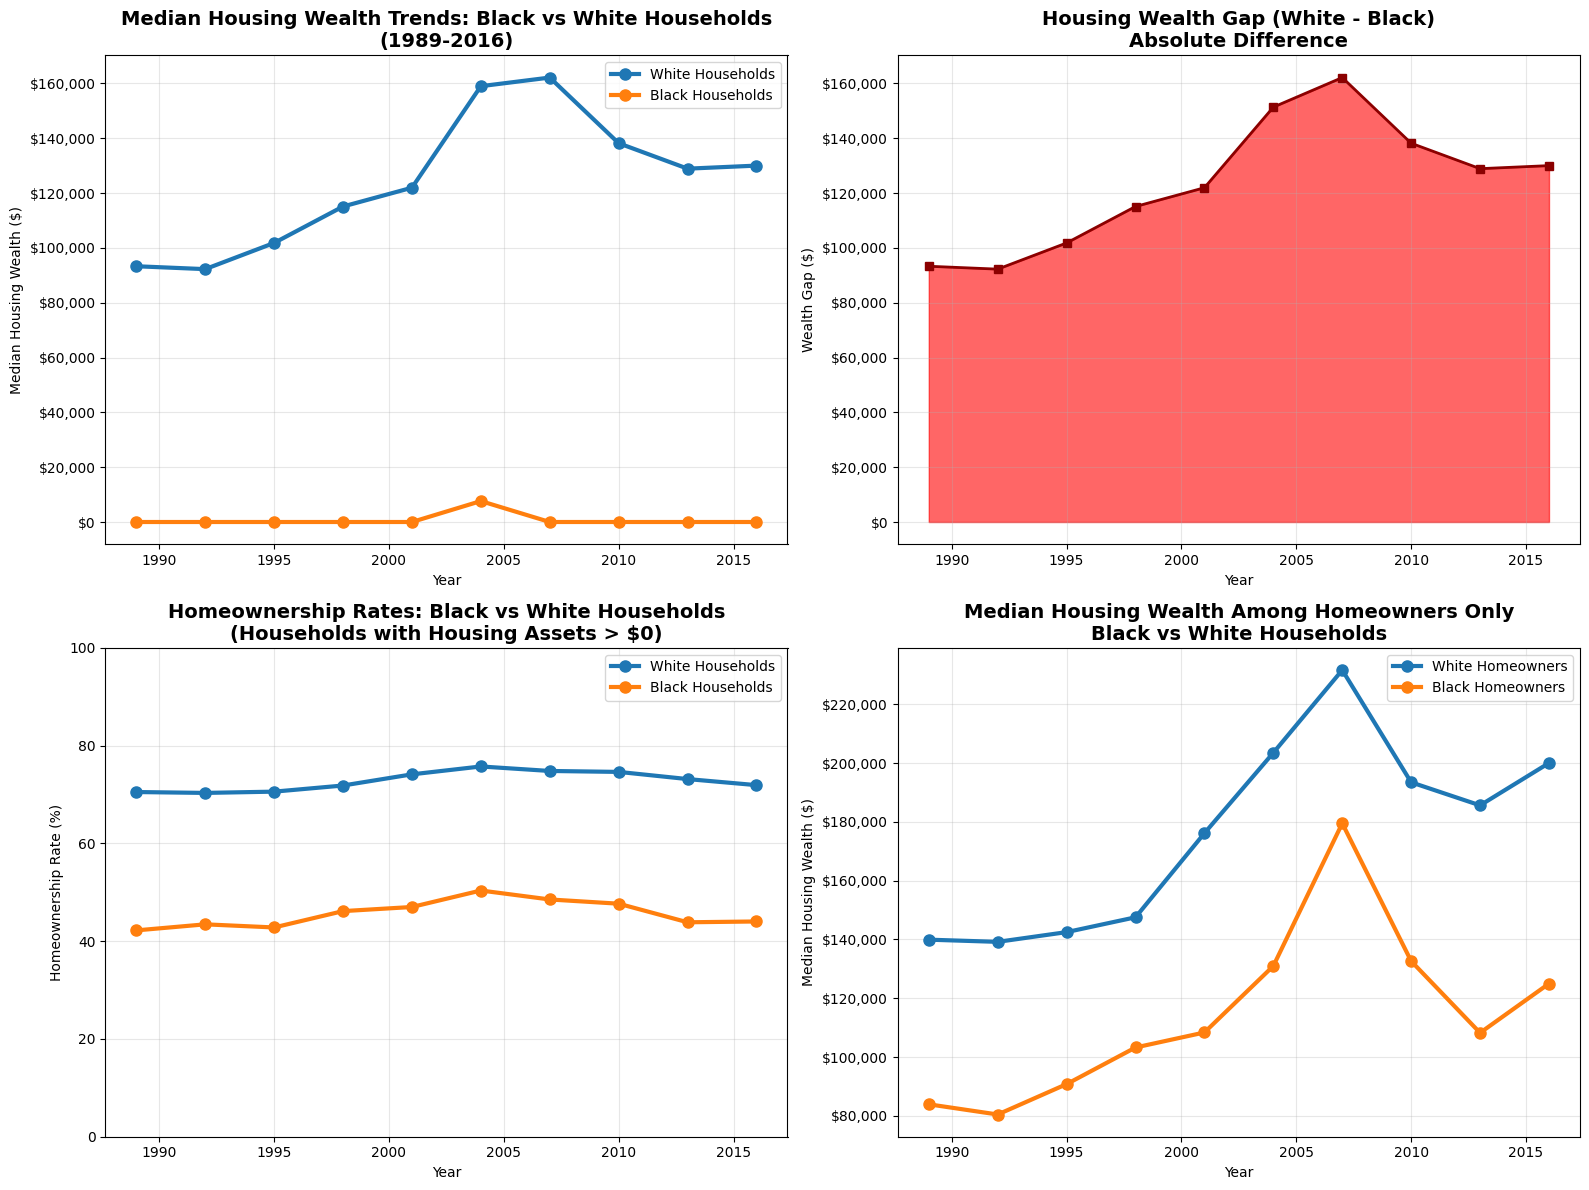
\includegraphics{main_files/figure-pdf/cell-14-output-1.png}

\begin{verbatim}
Homeownership rates by race and year:
race  black  white
year              
1989   42.2   70.5
1992   43.4   70.3
1995   42.8   70.6
1998   46.1   71.8
2001   47.0   74.1
2004   50.4   75.7
2007   48.5   74.8
2010   47.7   74.6
2013   43.9   73.2
2016   44.0   71.9
\end{verbatim}

\begin{Shaded}
\begin{Highlighting}[]
\CommentTok{\# Quantitative Analysis of Housing Wealth Trends}
\BuiltInTok{print}\NormalTok{(}\StringTok{"=== HOUSING WEALTH ANALYSIS: BLACK vs WHITE HOUSEHOLDS ===}\CharTok{\textbackslash{}n}\StringTok{"}\NormalTok{)}

\CommentTok{\# Calculate key statistics}
\BuiltInTok{print}\NormalTok{(}\StringTok{"1. MEDIAN HOUSING WEALTH AMONG ALL HOUSEHOLDS:"}\NormalTok{)}
\BuiltInTok{print}\NormalTok{(}\StringTok{"   White households (1989):"}\NormalTok{, }\SpecialStringTok{f"$}\SpecialCharTok{\{}\NormalTok{housing\_pivot}\SpecialCharTok{.}\NormalTok{loc[}\DecValTok{1989}\NormalTok{, }\StringTok{\textquotesingle{}white\textquotesingle{}}\NormalTok{]}\SpecialCharTok{:,.0f\}}\SpecialStringTok{"}\NormalTok{)}
\BuiltInTok{print}\NormalTok{(}\StringTok{"   White households (2016):"}\NormalTok{, }\SpecialStringTok{f"$}\SpecialCharTok{\{}\NormalTok{housing\_pivot}\SpecialCharTok{.}\NormalTok{loc[}\DecValTok{2016}\NormalTok{, }\StringTok{\textquotesingle{}white\textquotesingle{}}\NormalTok{]}\SpecialCharTok{:,.0f\}}\SpecialStringTok{"}\NormalTok{)}
\BuiltInTok{print}\NormalTok{(}\StringTok{"   Black households (1989):"}\NormalTok{, }\SpecialStringTok{f"$}\SpecialCharTok{\{}\NormalTok{housing\_pivot}\SpecialCharTok{.}\NormalTok{loc[}\DecValTok{1989}\NormalTok{, }\StringTok{\textquotesingle{}black\textquotesingle{}}\NormalTok{]}\SpecialCharTok{:,.0f\}}\SpecialStringTok{"}\NormalTok{)}
\BuiltInTok{print}\NormalTok{(}\StringTok{"   Black households (2016):"}\NormalTok{, }\SpecialStringTok{f"$}\SpecialCharTok{\{}\NormalTok{housing\_pivot}\SpecialCharTok{.}\NormalTok{loc[}\DecValTok{2016}\NormalTok{, }\StringTok{\textquotesingle{}black\textquotesingle{}}\NormalTok{]}\SpecialCharTok{:,.0f\}}\SpecialStringTok{"}\NormalTok{)}

\CommentTok{\# CAGR for housing wealth}
\NormalTok{white\_housing\_cagr }\OperatorTok{=}\NormalTok{ calculate\_cagr(housing\_pivot.loc[}\DecValTok{1989}\NormalTok{, }\StringTok{\textquotesingle{}white\textquotesingle{}}\NormalTok{], }
\NormalTok{                                   housing\_pivot.loc[}\DecValTok{2016}\NormalTok{, }\StringTok{\textquotesingle{}white\textquotesingle{}}\NormalTok{], years\_span)}
\BuiltInTok{print}\NormalTok{(}\SpecialStringTok{f"}\CharTok{\textbackslash{}n}\SpecialStringTok{   White Housing Wealth CAGR: }\SpecialCharTok{\{}\NormalTok{white\_housing\_cagr}\SpecialCharTok{:.2f\}}\SpecialStringTok{\% per year"}\NormalTok{)}

\CommentTok{\# Since Black median is mostly 0, calculate differently}
\NormalTok{black\_housing\_values }\OperatorTok{=}\NormalTok{ housing\_pivot[}\StringTok{\textquotesingle{}black\textquotesingle{}}\NormalTok{].dropna()}
\NormalTok{black\_positive\_years }\OperatorTok{=}\NormalTok{ black\_housing\_values[black\_housing\_values }\OperatorTok{\textgreater{}} \DecValTok{0}\NormalTok{]}
\BuiltInTok{print}\NormalTok{(}\SpecialStringTok{f"   Black households had positive median housing wealth in }\SpecialCharTok{\{}\BuiltInTok{len}\NormalTok{(black\_positive\_years)}\SpecialCharTok{\}}\SpecialStringTok{ of }\SpecialCharTok{\{}\BuiltInTok{len}\NormalTok{(black\_housing\_values)}\SpecialCharTok{\}}\SpecialStringTok{ years"}\NormalTok{)}

\BuiltInTok{print}\NormalTok{(}\StringTok{"}\CharTok{\textbackslash{}n}\StringTok{2. HOMEOWNERSHIP RATES:"}\NormalTok{)}
\BuiltInTok{print}\NormalTok{(}\StringTok{"   White households:"}\NormalTok{)}
\BuiltInTok{print}\NormalTok{(}\SpecialStringTok{f"     1989: }\SpecialCharTok{\{}\NormalTok{homeownership\_pivot}\SpecialCharTok{.}\NormalTok{loc[}\DecValTok{1989}\NormalTok{, }\StringTok{\textquotesingle{}white\textquotesingle{}}\NormalTok{]}\SpecialCharTok{:.1f\}}\SpecialStringTok{\%"}\NormalTok{)}
\BuiltInTok{print}\NormalTok{(}\SpecialStringTok{f"     2016: }\SpecialCharTok{\{}\NormalTok{homeownership\_pivot}\SpecialCharTok{.}\NormalTok{loc[}\DecValTok{2016}\NormalTok{, }\StringTok{\textquotesingle{}white\textquotesingle{}}\NormalTok{]}\SpecialCharTok{:.1f\}}\SpecialStringTok{\%"}\NormalTok{)}
\BuiltInTok{print}\NormalTok{(}\SpecialStringTok{f"     Average: }\SpecialCharTok{\{}\NormalTok{homeownership\_pivot[}\StringTok{\textquotesingle{}white\textquotesingle{}}\NormalTok{]}\SpecialCharTok{.}\NormalTok{mean()}\SpecialCharTok{:.1f\}}\SpecialStringTok{\%"}\NormalTok{)}

\BuiltInTok{print}\NormalTok{(}\StringTok{"   Black households:"}\NormalTok{)}
\BuiltInTok{print}\NormalTok{(}\SpecialStringTok{f"     1989: }\SpecialCharTok{\{}\NormalTok{homeownership\_pivot}\SpecialCharTok{.}\NormalTok{loc[}\DecValTok{1989}\NormalTok{, }\StringTok{\textquotesingle{}black\textquotesingle{}}\NormalTok{]}\SpecialCharTok{:.1f\}}\SpecialStringTok{\%"}\NormalTok{)}
\BuiltInTok{print}\NormalTok{(}\SpecialStringTok{f"     2016: }\SpecialCharTok{\{}\NormalTok{homeownership\_pivot}\SpecialCharTok{.}\NormalTok{loc[}\DecValTok{2016}\NormalTok{, }\StringTok{\textquotesingle{}black\textquotesingle{}}\NormalTok{]}\SpecialCharTok{:.1f\}}\SpecialStringTok{\%"}\NormalTok{)}
\BuiltInTok{print}\NormalTok{(}\SpecialStringTok{f"     Average: }\SpecialCharTok{\{}\NormalTok{homeownership\_pivot[}\StringTok{\textquotesingle{}black\textquotesingle{}}\NormalTok{]}\SpecialCharTok{.}\NormalTok{mean()}\SpecialCharTok{:.1f\}}\SpecialStringTok{\%"}\NormalTok{)}

\CommentTok{\# Homeownership gap}
\NormalTok{homeownership\_gap }\OperatorTok{=}\NormalTok{ homeownership\_pivot[}\StringTok{\textquotesingle{}white\textquotesingle{}}\NormalTok{] }\OperatorTok{{-}}\NormalTok{ homeownership\_pivot[}\StringTok{\textquotesingle{}black\textquotesingle{}}\NormalTok{]}
\BuiltInTok{print}\NormalTok{(}\SpecialStringTok{f"}\CharTok{\textbackslash{}n}\SpecialStringTok{   Homeownership Gap (White {-} Black):"}\NormalTok{)}
\BuiltInTok{print}\NormalTok{(}\SpecialStringTok{f"     1989: }\SpecialCharTok{\{}\NormalTok{homeownership\_gap}\SpecialCharTok{.}\NormalTok{loc[}\DecValTok{1989}\NormalTok{]}\SpecialCharTok{:.1f\}}\SpecialStringTok{ percentage points"}\NormalTok{)}
\BuiltInTok{print}\NormalTok{(}\SpecialStringTok{f"     2016: }\SpecialCharTok{\{}\NormalTok{homeownership\_gap}\SpecialCharTok{.}\NormalTok{loc[}\DecValTok{2016}\NormalTok{]}\SpecialCharTok{:.1f\}}\SpecialStringTok{ percentage points"}\NormalTok{)}
\BuiltInTok{print}\NormalTok{(}\SpecialStringTok{f"     Average: }\SpecialCharTok{\{}\NormalTok{homeownership\_gap}\SpecialCharTok{.}\NormalTok{mean()}\SpecialCharTok{:.1f\}}\SpecialStringTok{ percentage points"}\NormalTok{)}

\BuiltInTok{print}\NormalTok{(}\StringTok{"}\CharTok{\textbackslash{}n}\StringTok{3. MEDIAN HOUSING WEALTH AMONG HOMEOWNERS ONLY:"}\NormalTok{)}
\BuiltInTok{print}\NormalTok{(}\StringTok{"   White homeowners:"}\NormalTok{)}
\BuiltInTok{print}\NormalTok{(}\SpecialStringTok{f"     1989: $}\SpecialCharTok{\{}\NormalTok{homeowner\_pivot}\SpecialCharTok{.}\NormalTok{loc[}\DecValTok{1989}\NormalTok{, }\StringTok{\textquotesingle{}white\textquotesingle{}}\NormalTok{]}\SpecialCharTok{:,.0f\}}\SpecialStringTok{"}\NormalTok{)}
\BuiltInTok{print}\NormalTok{(}\SpecialStringTok{f"     2016: $}\SpecialCharTok{\{}\NormalTok{homeowner\_pivot}\SpecialCharTok{.}\NormalTok{loc[}\DecValTok{2016}\NormalTok{, }\StringTok{\textquotesingle{}white\textquotesingle{}}\NormalTok{]}\SpecialCharTok{:,.0f\}}\SpecialStringTok{"}\NormalTok{)}

\BuiltInTok{print}\NormalTok{(}\StringTok{"   Black homeowners:"}\NormalTok{)}
\BuiltInTok{print}\NormalTok{(}\SpecialStringTok{f"     1989: $}\SpecialCharTok{\{}\NormalTok{homeowner\_pivot}\SpecialCharTok{.}\NormalTok{loc[}\DecValTok{1989}\NormalTok{, }\StringTok{\textquotesingle{}black\textquotesingle{}}\NormalTok{]}\SpecialCharTok{:,.0f\}}\SpecialStringTok{"}\NormalTok{)}
\BuiltInTok{print}\NormalTok{(}\SpecialStringTok{f"     2016: $}\SpecialCharTok{\{}\NormalTok{homeowner\_pivot}\SpecialCharTok{.}\NormalTok{loc[}\DecValTok{2016}\NormalTok{, }\StringTok{\textquotesingle{}black\textquotesingle{}}\NormalTok{]}\SpecialCharTok{:,.0f\}}\SpecialStringTok{"}\NormalTok{)}

\CommentTok{\# Calculate ratio among homeowners}
\NormalTok{homeowner\_ratio\_1989 }\OperatorTok{=}\NormalTok{ homeowner\_pivot.loc[}\DecValTok{1989}\NormalTok{, }\StringTok{\textquotesingle{}white\textquotesingle{}}\NormalTok{] }\OperatorTok{/}\NormalTok{ homeowner\_pivot.loc[}\DecValTok{1989}\NormalTok{, }\StringTok{\textquotesingle{}black\textquotesingle{}}\NormalTok{]}
\NormalTok{homeowner\_ratio\_2016 }\OperatorTok{=}\NormalTok{ homeowner\_pivot.loc[}\DecValTok{2016}\NormalTok{, }\StringTok{\textquotesingle{}white\textquotesingle{}}\NormalTok{] }\OperatorTok{/}\NormalTok{ homeowner\_pivot.loc[}\DecValTok{2016}\NormalTok{, }\StringTok{\textquotesingle{}black\textquotesingle{}}\NormalTok{]}
\BuiltInTok{print}\NormalTok{(}\SpecialStringTok{f"}\CharTok{\textbackslash{}n}\SpecialStringTok{   White{-}to{-}Black Housing Wealth Ratio (among homeowners):"}\NormalTok{)}
\BuiltInTok{print}\NormalTok{(}\SpecialStringTok{f"     1989: }\SpecialCharTok{\{}\NormalTok{homeowner\_ratio\_1989}\SpecialCharTok{:.1f\}}\SpecialStringTok{"}\NormalTok{)}
\BuiltInTok{print}\NormalTok{(}\SpecialStringTok{f"     2016: }\SpecialCharTok{\{}\NormalTok{homeowner\_ratio\_2016}\SpecialCharTok{:.1f\}}\SpecialStringTok{"}\NormalTok{)}

\CommentTok{\# Housing wealth volatility}
\BuiltInTok{print}\NormalTok{(}\StringTok{"}\CharTok{\textbackslash{}n}\StringTok{4. HOUSING WEALTH VOLATILITY (Coefficient of Variation):"}\NormalTok{)}
\NormalTok{white\_housing\_cv }\OperatorTok{=}\NormalTok{ (housing\_pivot[}\StringTok{\textquotesingle{}white\textquotesingle{}}\NormalTok{].std() }\OperatorTok{/}\NormalTok{ housing\_pivot[}\StringTok{\textquotesingle{}white\textquotesingle{}}\NormalTok{].mean()) }\OperatorTok{*} \DecValTok{100}
\BuiltInTok{print}\NormalTok{(}\SpecialStringTok{f"   White households: }\SpecialCharTok{\{}\NormalTok{white\_housing\_cv}\SpecialCharTok{:.1f\}}\SpecialStringTok{\%"}\NormalTok{)}

\CommentTok{\# For Black households, calculate CV among homeowners since median is often 0}
\NormalTok{black\_homeowner\_cv }\OperatorTok{=}\NormalTok{ (homeowner\_pivot[}\StringTok{\textquotesingle{}black\textquotesingle{}}\NormalTok{].std() }\OperatorTok{/}\NormalTok{ homeowner\_pivot[}\StringTok{\textquotesingle{}black\textquotesingle{}}\NormalTok{].mean()) }\OperatorTok{*} \DecValTok{100}
\BuiltInTok{print}\NormalTok{(}\SpecialStringTok{f"   Black homeowners: }\SpecialCharTok{\{}\NormalTok{black\_homeowner\_cv}\SpecialCharTok{:.1f\}}\SpecialStringTok{\%"}\NormalTok{)}

\BuiltInTok{print}\NormalTok{(}\StringTok{"}\CharTok{\textbackslash{}n}\StringTok{=== END HOUSING WEALTH ANALYSIS ==="}\NormalTok{)  }
\end{Highlighting}
\end{Shaded}

\begin{verbatim}
=== HOUSING WEALTH ANALYSIS: BLACK vs WHITE HOUSEHOLDS ===

1. MEDIAN HOUSING WEALTH AMONG ALL HOUSEHOLDS:
   White households (1989): $93,293
   White households (2016): $130,000
   Black households (1989): $0
   Black households (2016): $0

   White Housing Wealth CAGR: 1.24% per year
   Black households had positive median housing wealth in 1 of 10 years

2. HOMEOWNERSHIP RATES:
   White households:
     1989: 70.5%
     2016: 71.9%
     Average: 72.8%
   Black households:
     1989: 42.2%
     2016: 44.0%
     Average: 45.6%

   Homeownership Gap (White - Black):
     1989: 28.3 percentage points
     2016: 27.9 percentage points
     Average: 27.2 percentage points

3. MEDIAN HOUSING WEALTH AMONG HOMEOWNERS ONLY:
   White homeowners:
     1989: $139,940
     2016: $200,000
   Black homeowners:
     1989: $83,964
     2016: $125,000

   White-to-Black Housing Wealth Ratio (among homeowners):
     1989: 1.7
     2016: 1.6

4. HOUSING WEALTH VOLATILITY (Coefficient of Variation):
   White households: 19.8%
   Black homeowners: 25.7%

=== END HOUSING WEALTH ANALYSIS ===
\end{verbatim}

\begin{Shaded}
\begin{Highlighting}[]
\CommentTok{\# HOMEOWNERS AGED 25+ ANALYSIS: Housing vs Non{-}Housing Wealth}
\BuiltInTok{print}\NormalTok{(}\StringTok{"=== HOMEOWNERS AGED 25+ WEALTH ANALYSIS ===}\CharTok{\textbackslash{}n}\StringTok{"}\NormalTok{)}

\CommentTok{\# Filter to homeowners aged 25 or older (those with housing assets \textgreater{} 0 and age \textgreater{}= 25)}
\NormalTok{homeowners\_25plus }\OperatorTok{=}\NormalTok{ df[(df[}\StringTok{\textquotesingle{}asset\_housing\textquotesingle{}}\NormalTok{] }\OperatorTok{\textgreater{}} \DecValTok{0}\NormalTok{) }\OperatorTok{\&}\NormalTok{ (df[}\StringTok{\textquotesingle{}age\textquotesingle{}}\NormalTok{] }\OperatorTok{\textgreater{}=} \DecValTok{25}\NormalTok{)].copy()}

\BuiltInTok{print}\NormalTok{(}\SpecialStringTok{f"Filtered dataset: }\SpecialCharTok{\{}\BuiltInTok{len}\NormalTok{(homeowners\_25plus)}\SpecialCharTok{:,\}}\SpecialStringTok{ homeowners aged 25+ out of }\SpecialCharTok{\{}\BuiltInTok{len}\NormalTok{(df)}\SpecialCharTok{:,\}}\SpecialStringTok{ total observations"}\NormalTok{)}
\BuiltInTok{print}\NormalTok{(}\SpecialStringTok{f"Represents }\SpecialCharTok{\{}\BuiltInTok{len}\NormalTok{(homeowners\_25plus)}\OperatorTok{/}\BuiltInTok{len}\NormalTok{(df)}\OperatorTok{*}\DecValTok{100}\SpecialCharTok{:.1f\}}\SpecialStringTok{\% of the full dataset"}\NormalTok{)}

\CommentTok{\# Create non{-}housing wealth variable}
\NormalTok{homeowners\_25plus[}\StringTok{\textquotesingle{}non\_housing\_wealth\textquotesingle{}}\NormalTok{] }\OperatorTok{=}\NormalTok{ homeowners\_25plus[}\StringTok{\textquotesingle{}asset\_total\textquotesingle{}}\NormalTok{] }\OperatorTok{{-}}\NormalTok{ homeowners\_25plus[}\StringTok{\textquotesingle{}asset\_housing\textquotesingle{}}\NormalTok{] }\OperatorTok{{-}}\NormalTok{ homeowners\_25plus[}\StringTok{\textquotesingle{}debt\_total\textquotesingle{}}\NormalTok{] }\OperatorTok{+}\NormalTok{ homeowners\_25plus[}\StringTok{\textquotesingle{}debt\_housing\textquotesingle{}}\NormalTok{]}

\BuiltInTok{print}\NormalTok{(}\SpecialStringTok{f"}\CharTok{\textbackslash{}n}\SpecialStringTok{Race distribution among homeowners 25+:"}\NormalTok{)}
\NormalTok{race\_dist }\OperatorTok{=}\NormalTok{ homeowners\_25plus.groupby(}\StringTok{\textquotesingle{}race\textquotesingle{}}\NormalTok{).size().sort\_values(ascending}\OperatorTok{=}\VariableTok{False}\NormalTok{)}
\ControlFlowTok{for}\NormalTok{ race, count }\KeywordTok{in}\NormalTok{ race\_dist.items():}
\NormalTok{    pct }\OperatorTok{=}\NormalTok{ (count }\OperatorTok{/} \BuiltInTok{len}\NormalTok{(homeowners\_25plus)) }\OperatorTok{*} \DecValTok{100}
    \BuiltInTok{print}\NormalTok{(}\SpecialStringTok{f"  }\SpecialCharTok{\{}\NormalTok{race}\SpecialCharTok{.}\NormalTok{title()}\SpecialCharTok{\}}\SpecialStringTok{: }\SpecialCharTok{\{}\NormalTok{count}\SpecialCharTok{:,\}}\SpecialStringTok{ (}\SpecialCharTok{\{}\NormalTok{pct}\SpecialCharTok{:.1f\}}\SpecialStringTok{\%)"}\NormalTok{)}

\CommentTok{\# Focus on Black and White homeowners for detailed analysis}
\NormalTok{target\_races }\OperatorTok{=}\NormalTok{ [}\StringTok{\textquotesingle{}black\textquotesingle{}}\NormalTok{, }\StringTok{\textquotesingle{}white\textquotesingle{}}\NormalTok{]}
\NormalTok{bw\_homeowners }\OperatorTok{=}\NormalTok{ homeowners\_25plus[homeowners\_25plus[}\StringTok{\textquotesingle{}race\textquotesingle{}}\NormalTok{].isin(target\_races)].copy()}

\BuiltInTok{print}\NormalTok{(}\SpecialStringTok{f"}\CharTok{\textbackslash{}n}\SpecialStringTok{Black and White homeowners 25+: }\SpecialCharTok{\{}\BuiltInTok{len}\NormalTok{(bw\_homeowners)}\SpecialCharTok{:,\}}\SpecialStringTok{ observations"}\NormalTok{)}

\CommentTok{\# Calculate median housing and non{-}housing wealth by race and year}
\NormalTok{housing\_nonhousing\_data }\OperatorTok{=}\NormalTok{ []}

\ControlFlowTok{for}\NormalTok{ year }\KeywordTok{in} \BuiltInTok{sorted}\NormalTok{(bw\_homeowners[}\StringTok{\textquotesingle{}year\textquotesingle{}}\NormalTok{].unique()):}
    \ControlFlowTok{for}\NormalTok{ race }\KeywordTok{in}\NormalTok{ target\_races:}
\NormalTok{        subset }\OperatorTok{=}\NormalTok{ bw\_homeowners[(bw\_homeowners[}\StringTok{\textquotesingle{}year\textquotesingle{}}\NormalTok{] }\OperatorTok{==}\NormalTok{ year) }\OperatorTok{\&}\NormalTok{ (bw\_homeowners[}\StringTok{\textquotesingle{}race\textquotesingle{}}\NormalTok{] }\OperatorTok{==}\NormalTok{ race)]}
        \ControlFlowTok{if} \BuiltInTok{len}\NormalTok{(subset) }\OperatorTok{\textgreater{}} \DecValTok{0}\NormalTok{:}
            \CommentTok{\# Housing wealth}
\NormalTok{            housing\_wealth\_med }\OperatorTok{=}\NormalTok{ weighted\_median(subset[}\StringTok{\textquotesingle{}asset\_housing\textquotesingle{}}\NormalTok{].values, subset[}\StringTok{\textquotesingle{}weight\textquotesingle{}}\NormalTok{].values)}
            
            \CommentTok{\# Non{-}housing wealth}
\NormalTok{            nonhousing\_wealth\_med }\OperatorTok{=}\NormalTok{ weighted\_median(subset[}\StringTok{\textquotesingle{}non\_housing\_wealth\textquotesingle{}}\NormalTok{].values, subset[}\StringTok{\textquotesingle{}weight\textquotesingle{}}\NormalTok{].values)}
            
\NormalTok{            housing\_nonhousing\_data.append(\{}
                \StringTok{\textquotesingle{}year\textquotesingle{}}\NormalTok{: year,}
                \StringTok{\textquotesingle{}race\textquotesingle{}}\NormalTok{: race,}
                \StringTok{\textquotesingle{}median\_housing\_wealth\textquotesingle{}}\NormalTok{: housing\_wealth\_med,}
                \StringTok{\textquotesingle{}median\_nonhousing\_wealth\textquotesingle{}}\NormalTok{: nonhousing\_wealth\_med,}
                \StringTok{\textquotesingle{}sample\_size\textquotesingle{}}\NormalTok{: }\BuiltInTok{len}\NormalTok{(subset)}
\NormalTok{            \})}

\NormalTok{hn\_df }\OperatorTok{=}\NormalTok{ pd.DataFrame(housing\_nonhousing\_data)}

\CommentTok{\# Create pivot tables}
\NormalTok{housing\_pivot\_owners }\OperatorTok{=}\NormalTok{ hn\_df.pivot(index}\OperatorTok{=}\StringTok{\textquotesingle{}year\textquotesingle{}}\NormalTok{, columns}\OperatorTok{=}\StringTok{\textquotesingle{}race\textquotesingle{}}\NormalTok{, values}\OperatorTok{=}\StringTok{\textquotesingle{}median\_housing\_wealth\textquotesingle{}}\NormalTok{)}
\NormalTok{nonhousing\_pivot\_owners }\OperatorTok{=}\NormalTok{ hn\_df.pivot(index}\OperatorTok{=}\StringTok{\textquotesingle{}year\textquotesingle{}}\NormalTok{, columns}\OperatorTok{=}\StringTok{\textquotesingle{}race\textquotesingle{}}\NormalTok{, values}\OperatorTok{=}\StringTok{\textquotesingle{}median\_nonhousing\_wealth\textquotesingle{}}\NormalTok{)}

\BuiltInTok{print}\NormalTok{(}\StringTok{"}\CharTok{\textbackslash{}n}\StringTok{1. MEDIAN HOUSING WEALTH AMONG HOMEOWNERS 25+ (by race and year):"}\NormalTok{)}
\BuiltInTok{print}\NormalTok{(housing\_pivot\_owners.}\BuiltInTok{round}\NormalTok{(}\DecValTok{0}\NormalTok{))}

\BuiltInTok{print}\NormalTok{(}\StringTok{"}\CharTok{\textbackslash{}n}\StringTok{2. MEDIAN NON{-}HOUSING WEALTH AMONG HOMEOWNERS 25+ (by race and year):"}\NormalTok{)}
\BuiltInTok{print}\NormalTok{(nonhousing\_pivot\_owners.}\BuiltInTok{round}\NormalTok{(}\DecValTok{0}\NormalTok{))}
\end{Highlighting}
\end{Shaded}

\begin{verbatim}
=== HOMEOWNERS AGED 25+ WEALTH ANALYSIS ===

Filtered dataset: 33,292 homeowners aged 25+ out of 47,776 total observations
Represents 69.7% of the full dataset

Race distribution among homeowners 25+:
  White: 28,370 (85.2%)
  Black: 2,105 (6.3%)
  Hispanic: 1,570 (4.7%)
  Other: 1,247 (3.7%)

Black and White homeowners 25+: 30,475 observations

1. MEDIAN HOUSING WEALTH AMONG HOMEOWNERS 25+ (by race and year):
race     black     white
year                    
1989   83964.0  139940.0
1992   80499.0  142551.0
1995   93960.0  144072.0
1998  103282.0  147546.0
2001  108388.0  176131.0
2004  130994.0  209844.0
2007  173702.0  231603.0
2010  132639.0  193433.0
2013  108266.0  185599.0
2016  125000.0  200000.0

2. MEDIAN NON-HOUSING WEALTH AMONG HOMEOWNERS 25+ (by race and year):
race    black     white
year                   
1989  12128.0   81725.0
1992  16603.0   70185.0
1995  20828.0   80179.0
1998  27517.0  113758.0
2001  32462.0  146053.0
2004  20984.0  121964.0
2007  40299.0  124371.0
2010  23720.0  110643.0
2013  18869.0  124764.0
2016  29540.0  144730.0
\end{verbatim}

\begin{Shaded}
\begin{Highlighting}[]
\CommentTok{\# Create comprehensive visualizations for homeowners 25+}
\NormalTok{fig, ((ax1, ax2), (ax3, ax4)) }\OperatorTok{=}\NormalTok{ plt.subplots(}\DecValTok{2}\NormalTok{, }\DecValTok{2}\NormalTok{, figsize}\OperatorTok{=}\NormalTok{(}\DecValTok{16}\NormalTok{, }\DecValTok{12}\NormalTok{))}

\CommentTok{\# Plot 1: Housing wealth trends for homeowners 25+}
\NormalTok{colors\_race }\OperatorTok{=}\NormalTok{ [}\StringTok{\textquotesingle{}\#1f77b4\textquotesingle{}}\NormalTok{, }\StringTok{\textquotesingle{}\#ff7f0e\textquotesingle{}}\NormalTok{]  }\CommentTok{\# Blue for White, Orange for Black}
\ControlFlowTok{for}\NormalTok{ i, race }\KeywordTok{in} \BuiltInTok{enumerate}\NormalTok{([}\StringTok{\textquotesingle{}white\textquotesingle{}}\NormalTok{, }\StringTok{\textquotesingle{}black\textquotesingle{}}\NormalTok{]):}
    \ControlFlowTok{if}\NormalTok{ race }\KeywordTok{in}\NormalTok{ housing\_pivot\_owners.columns:}
\NormalTok{        ax1.plot(housing\_pivot\_owners.index, housing\_pivot\_owners[race], marker}\OperatorTok{=}\StringTok{\textquotesingle{}o\textquotesingle{}}\NormalTok{, linewidth}\OperatorTok{=}\DecValTok{3}\NormalTok{, }
\NormalTok{                label}\OperatorTok{=}\SpecialStringTok{f\textquotesingle{}}\SpecialCharTok{\{}\NormalTok{race}\SpecialCharTok{.}\NormalTok{title()}\SpecialCharTok{\}}\SpecialStringTok{ Homeowners\textquotesingle{}}\NormalTok{, color}\OperatorTok{=}\NormalTok{colors\_race[i], markersize}\OperatorTok{=}\DecValTok{8}\NormalTok{)}

\NormalTok{ax1.set\_title(}\StringTok{\textquotesingle{}Median Housing Wealth: Black vs White Homeowners 25+}\CharTok{\textbackslash{}n}\StringTok{(1989{-}2016)\textquotesingle{}}\NormalTok{, }
\NormalTok{              fontsize}\OperatorTok{=}\DecValTok{14}\NormalTok{, fontweight}\OperatorTok{=}\StringTok{\textquotesingle{}bold\textquotesingle{}}\NormalTok{)}
\NormalTok{ax1.set\_xlabel(}\StringTok{\textquotesingle{}Year\textquotesingle{}}\NormalTok{)}
\NormalTok{ax1.set\_ylabel(}\StringTok{\textquotesingle{}Median Housing Wealth ($)\textquotesingle{}}\NormalTok{)}
\NormalTok{ax1.legend()}
\NormalTok{ax1.grid(}\VariableTok{True}\NormalTok{, alpha}\OperatorTok{=}\FloatTok{0.3}\NormalTok{)}
\NormalTok{ax1.yaxis.set\_major\_formatter(plt.FuncFormatter(}\KeywordTok{lambda}\NormalTok{ x, p: }\SpecialStringTok{f\textquotesingle{}$}\SpecialCharTok{\{}\NormalTok{x}\SpecialCharTok{:,.0f\}}\SpecialStringTok{\textquotesingle{}}\NormalTok{))}

\CommentTok{\# Plot 2: Non{-}housing wealth trends for homeowners 25+}
\ControlFlowTok{for}\NormalTok{ i, race }\KeywordTok{in} \BuiltInTok{enumerate}\NormalTok{([}\StringTok{\textquotesingle{}white\textquotesingle{}}\NormalTok{, }\StringTok{\textquotesingle{}black\textquotesingle{}}\NormalTok{]):}
    \ControlFlowTok{if}\NormalTok{ race }\KeywordTok{in}\NormalTok{ nonhousing\_pivot\_owners.columns:}
\NormalTok{        ax2.plot(nonhousing\_pivot\_owners.index, nonhousing\_pivot\_owners[race], marker}\OperatorTok{=}\StringTok{\textquotesingle{}s\textquotesingle{}}\NormalTok{, linewidth}\OperatorTok{=}\DecValTok{3}\NormalTok{, }
\NormalTok{                label}\OperatorTok{=}\SpecialStringTok{f\textquotesingle{}}\SpecialCharTok{\{}\NormalTok{race}\SpecialCharTok{.}\NormalTok{title()}\SpecialCharTok{\}}\SpecialStringTok{ Homeowners\textquotesingle{}}\NormalTok{, color}\OperatorTok{=}\NormalTok{colors\_race[i], markersize}\OperatorTok{=}\DecValTok{8}\NormalTok{)}

\NormalTok{ax2.set\_title(}\StringTok{\textquotesingle{}Median Non{-}Housing Wealth: Black vs White Homeowners 25+}\CharTok{\textbackslash{}n}\StringTok{(1989{-}2016)\textquotesingle{}}\NormalTok{, }
\NormalTok{              fontsize}\OperatorTok{=}\DecValTok{14}\NormalTok{, fontweight}\OperatorTok{=}\StringTok{\textquotesingle{}bold\textquotesingle{}}\NormalTok{)}
\NormalTok{ax2.set\_xlabel(}\StringTok{\textquotesingle{}Year\textquotesingle{}}\NormalTok{)}
\NormalTok{ax2.set\_ylabel(}\StringTok{\textquotesingle{}Median Non{-}Housing Wealth ($)\textquotesingle{}}\NormalTok{)}
\NormalTok{ax2.legend()}
\NormalTok{ax2.grid(}\VariableTok{True}\NormalTok{, alpha}\OperatorTok{=}\FloatTok{0.3}\NormalTok{)}
\NormalTok{ax2.yaxis.set\_major\_formatter(plt.FuncFormatter(}\KeywordTok{lambda}\NormalTok{ x, p: }\SpecialStringTok{f\textquotesingle{}$}\SpecialCharTok{\{}\NormalTok{x}\SpecialCharTok{:,.0f\}}\SpecialStringTok{\textquotesingle{}}\NormalTok{))}

\CommentTok{\# Plot 3: Housing wealth gap between races}
\NormalTok{housing\_gap\_owners }\OperatorTok{=}\NormalTok{ housing\_pivot\_owners[}\StringTok{\textquotesingle{}white\textquotesingle{}}\NormalTok{] }\OperatorTok{{-}}\NormalTok{ housing\_pivot\_owners[}\StringTok{\textquotesingle{}black\textquotesingle{}}\NormalTok{]}
\NormalTok{ax3.fill\_between(housing\_gap\_owners.index, }\DecValTok{0}\NormalTok{, housing\_gap\_owners.values, alpha}\OperatorTok{=}\FloatTok{0.6}\NormalTok{, color}\OperatorTok{=}\StringTok{\textquotesingle{}red\textquotesingle{}}\NormalTok{)}
\NormalTok{ax3.plot(housing\_gap\_owners.index, housing\_gap\_owners.values, marker}\OperatorTok{=}\StringTok{\textquotesingle{}o\textquotesingle{}}\NormalTok{, linewidth}\OperatorTok{=}\DecValTok{2}\NormalTok{, }
\NormalTok{         color}\OperatorTok{=}\StringTok{\textquotesingle{}darkred\textquotesingle{}}\NormalTok{, markersize}\OperatorTok{=}\DecValTok{6}\NormalTok{)}
\NormalTok{ax3.set\_title(}\StringTok{\textquotesingle{}Housing Wealth Gap Among Homeowners 25+}\CharTok{\textbackslash{}n}\StringTok{(White {-} Black)\textquotesingle{}}\NormalTok{, }
\NormalTok{              fontsize}\OperatorTok{=}\DecValTok{14}\NormalTok{, fontweight}\OperatorTok{=}\StringTok{\textquotesingle{}bold\textquotesingle{}}\NormalTok{)}
\NormalTok{ax3.set\_xlabel(}\StringTok{\textquotesingle{}Year\textquotesingle{}}\NormalTok{)}
\NormalTok{ax3.set\_ylabel(}\StringTok{\textquotesingle{}Housing Wealth Gap ($)\textquotesingle{}}\NormalTok{)}
\NormalTok{ax3.grid(}\VariableTok{True}\NormalTok{, alpha}\OperatorTok{=}\FloatTok{0.3}\NormalTok{)}
\NormalTok{ax3.yaxis.set\_major\_formatter(plt.FuncFormatter(}\KeywordTok{lambda}\NormalTok{ x, p: }\SpecialStringTok{f\textquotesingle{}$}\SpecialCharTok{\{}\NormalTok{x}\SpecialCharTok{:,.0f\}}\SpecialStringTok{\textquotesingle{}}\NormalTok{))}

\CommentTok{\# Plot 4: Non{-}housing wealth gap between races}
\NormalTok{nonhousing\_gap\_owners }\OperatorTok{=}\NormalTok{ nonhousing\_pivot\_owners[}\StringTok{\textquotesingle{}white\textquotesingle{}}\NormalTok{] }\OperatorTok{{-}}\NormalTok{ nonhousing\_pivot\_owners[}\StringTok{\textquotesingle{}black\textquotesingle{}}\NormalTok{]}
\NormalTok{ax4.fill\_between(nonhousing\_gap\_owners.index, }\DecValTok{0}\NormalTok{, nonhousing\_gap\_owners.values, alpha}\OperatorTok{=}\FloatTok{0.6}\NormalTok{, color}\OperatorTok{=}\StringTok{\textquotesingle{}purple\textquotesingle{}}\NormalTok{)}
\NormalTok{ax4.plot(nonhousing\_gap\_owners.index, nonhousing\_gap\_owners.values, marker}\OperatorTok{=}\StringTok{\textquotesingle{}s\textquotesingle{}}\NormalTok{, linewidth}\OperatorTok{=}\DecValTok{2}\NormalTok{, }
\NormalTok{         color}\OperatorTok{=}\StringTok{\textquotesingle{}darkviolet\textquotesingle{}}\NormalTok{, markersize}\OperatorTok{=}\DecValTok{6}\NormalTok{)}
\NormalTok{ax4.set\_title(}\StringTok{\textquotesingle{}Non{-}Housing Wealth Gap Among Homeowners 25+}\CharTok{\textbackslash{}n}\StringTok{(White {-} Black)\textquotesingle{}}\NormalTok{, }
\NormalTok{              fontsize}\OperatorTok{=}\DecValTok{14}\NormalTok{, fontweight}\OperatorTok{=}\StringTok{\textquotesingle{}bold\textquotesingle{}}\NormalTok{)}
\NormalTok{ax4.set\_xlabel(}\StringTok{\textquotesingle{}Year\textquotesingle{}}\NormalTok{)}
\NormalTok{ax4.set\_ylabel(}\StringTok{\textquotesingle{}Non{-}Housing Wealth Gap ($)\textquotesingle{}}\NormalTok{)}
\NormalTok{ax4.grid(}\VariableTok{True}\NormalTok{, alpha}\OperatorTok{=}\FloatTok{0.3}\NormalTok{)}
\NormalTok{ax4.yaxis.set\_major\_formatter(plt.FuncFormatter(}\KeywordTok{lambda}\NormalTok{ x, p: }\SpecialStringTok{f\textquotesingle{}$}\SpecialCharTok{\{}\NormalTok{x}\SpecialCharTok{:,.0f\}}\SpecialStringTok{\textquotesingle{}}\NormalTok{))}

\NormalTok{plt.tight\_layout()}
\NormalTok{plt.show()}

\CommentTok{\# FINANCIAL CRISIS ANALYSIS (2007 as base period)}
\BuiltInTok{print}\NormalTok{(}\StringTok{"}\CharTok{\textbackslash{}n}\StringTok{=== FINANCIAL CRISIS IMPACT ANALYSIS (2007 Base) ===}\CharTok{\textbackslash{}n}\StringTok{"}\NormalTok{)}

\CommentTok{\# Get 2007 and 2010 values for comparison}
\NormalTok{crisis\_years }\OperatorTok{=}\NormalTok{ [}\DecValTok{2007}\NormalTok{, }\DecValTok{2010}\NormalTok{]}

\CommentTok{\# Housing wealth losses}
\BuiltInTok{print}\NormalTok{(}\StringTok{"3. HOUSING WEALTH LOSSES (2007{-}2010):"}\NormalTok{)}
\ControlFlowTok{for}\NormalTok{ race }\KeywordTok{in}\NormalTok{ [}\StringTok{\textquotesingle{}white\textquotesingle{}}\NormalTok{, }\StringTok{\textquotesingle{}black\textquotesingle{}}\NormalTok{]:}
    \ControlFlowTok{if}\NormalTok{ race }\KeywordTok{in}\NormalTok{ housing\_pivot\_owners.columns:}
\NormalTok{        housing\_2007 }\OperatorTok{=}\NormalTok{ housing\_pivot\_owners.loc[}\DecValTok{2007}\NormalTok{, race]}
\NormalTok{        housing\_2010 }\OperatorTok{=}\NormalTok{ housing\_pivot\_owners.loc[}\DecValTok{2010}\NormalTok{, race]}
        
        \CommentTok{\# Dollar loss}
\NormalTok{        dollar\_loss }\OperatorTok{=}\NormalTok{ housing\_2007 }\OperatorTok{{-}}\NormalTok{ housing\_2010}
        
        \CommentTok{\# Proportional loss}
\NormalTok{        prop\_loss }\OperatorTok{=}\NormalTok{ (dollar\_loss }\OperatorTok{/}\NormalTok{ housing\_2007) }\OperatorTok{*} \DecValTok{100}
        
        \BuiltInTok{print}\NormalTok{(}\SpecialStringTok{f"   }\SpecialCharTok{\{}\NormalTok{race}\SpecialCharTok{.}\NormalTok{title()}\SpecialCharTok{\}}\SpecialStringTok{ homeowners 25+:"}\NormalTok{)}
        \BuiltInTok{print}\NormalTok{(}\SpecialStringTok{f"     2007: $}\SpecialCharTok{\{}\NormalTok{housing\_2007}\SpecialCharTok{:,.0f\}}\SpecialStringTok{"}\NormalTok{)}
        \BuiltInTok{print}\NormalTok{(}\SpecialStringTok{f"     2010: $}\SpecialCharTok{\{}\NormalTok{housing\_2010}\SpecialCharTok{:,.0f\}}\SpecialStringTok{"}\NormalTok{)}
        \BuiltInTok{print}\NormalTok{(}\SpecialStringTok{f"     Dollar loss: $}\SpecialCharTok{\{}\NormalTok{dollar\_loss}\SpecialCharTok{:,.0f\}}\SpecialStringTok{"}\NormalTok{)}
        \BuiltInTok{print}\NormalTok{(}\SpecialStringTok{f"     Proportional loss: }\SpecialCharTok{\{}\NormalTok{prop\_loss}\SpecialCharTok{:.1f\}}\SpecialStringTok{\%"}\NormalTok{)}
        \BuiltInTok{print}\NormalTok{()}

\CommentTok{\# Non{-}housing wealth changes}
\BuiltInTok{print}\NormalTok{(}\StringTok{"4. NON{-}HOUSING WEALTH CHANGES (2007{-}2010):"}\NormalTok{)}
\ControlFlowTok{for}\NormalTok{ race }\KeywordTok{in}\NormalTok{ [}\StringTok{\textquotesingle{}white\textquotesingle{}}\NormalTok{, }\StringTok{\textquotesingle{}black\textquotesingle{}}\NormalTok{]:}
    \ControlFlowTok{if}\NormalTok{ race }\KeywordTok{in}\NormalTok{ nonhousing\_pivot\_owners.columns:}
\NormalTok{        nonhousing\_2007 }\OperatorTok{=}\NormalTok{ nonhousing\_pivot\_owners.loc[}\DecValTok{2007}\NormalTok{, race]}
\NormalTok{        nonhousing\_2010 }\OperatorTok{=}\NormalTok{ nonhousing\_pivot\_owners.loc[}\DecValTok{2010}\NormalTok{, race]}
        
        \CommentTok{\# Dollar change}
\NormalTok{        dollar\_change }\OperatorTok{=}\NormalTok{ nonhousing\_2010 }\OperatorTok{{-}}\NormalTok{ nonhousing\_2007}
        
        \CommentTok{\# Proportional change (handle negative values carefully)}
        \ControlFlowTok{if}\NormalTok{ nonhousing\_2007 }\OperatorTok{!=} \DecValTok{0}\NormalTok{:}
\NormalTok{            prop\_change }\OperatorTok{=}\NormalTok{ (dollar\_change }\OperatorTok{/} \BuiltInTok{abs}\NormalTok{(nonhousing\_2007)) }\OperatorTok{*} \DecValTok{100}
        \ControlFlowTok{else}\NormalTok{:}
\NormalTok{            prop\_change }\OperatorTok{=}\NormalTok{ np.nan}
        
        \BuiltInTok{print}\NormalTok{(}\SpecialStringTok{f"   }\SpecialCharTok{\{}\NormalTok{race}\SpecialCharTok{.}\NormalTok{title()}\SpecialCharTok{\}}\SpecialStringTok{ homeowners 25+:"}\NormalTok{)}
        \BuiltInTok{print}\NormalTok{(}\SpecialStringTok{f"     2007: $}\SpecialCharTok{\{}\NormalTok{nonhousing\_2007}\SpecialCharTok{:,.0f\}}\SpecialStringTok{"}\NormalTok{)}
        \BuiltInTok{print}\NormalTok{(}\SpecialStringTok{f"     2010: $}\SpecialCharTok{\{}\NormalTok{nonhousing\_2010}\SpecialCharTok{:,.0f\}}\SpecialStringTok{"}\NormalTok{)}
        \BuiltInTok{print}\NormalTok{(}\SpecialStringTok{f"     Dollar change: $}\SpecialCharTok{\{}\NormalTok{dollar\_change}\SpecialCharTok{:,.0f\}}\SpecialStringTok{"}\NormalTok{)}
        \ControlFlowTok{if} \KeywordTok{not}\NormalTok{ np.isnan(prop\_change):}
            \BuiltInTok{print}\NormalTok{(}\SpecialStringTok{f"     Proportional change: }\SpecialCharTok{\{}\NormalTok{prop\_change}\SpecialCharTok{:.1f\}}\SpecialStringTok{\%"}\NormalTok{)}
        \ControlFlowTok{else}\NormalTok{:}
            \BuiltInTok{print}\NormalTok{(}\SpecialStringTok{f"     Proportional change: N/A (zero base)"}\NormalTok{)}
        \BuiltInTok{print}\NormalTok{()}

\CommentTok{\# Summary comparison}
\BuiltInTok{print}\NormalTok{(}\StringTok{"5. CRISIS IMPACT SUMMARY:"}\NormalTok{)}
\NormalTok{white\_housing\_loss }\OperatorTok{=}\NormalTok{ housing\_pivot\_owners.loc[}\DecValTok{2007}\NormalTok{, }\StringTok{\textquotesingle{}white\textquotesingle{}}\NormalTok{] }\OperatorTok{{-}}\NormalTok{ housing\_pivot\_owners.loc[}\DecValTok{2010}\NormalTok{, }\StringTok{\textquotesingle{}white\textquotesingle{}}\NormalTok{]}
\NormalTok{black\_housing\_loss }\OperatorTok{=}\NormalTok{ housing\_pivot\_owners.loc[}\DecValTok{2007}\NormalTok{, }\StringTok{\textquotesingle{}black\textquotesingle{}}\NormalTok{] }\OperatorTok{{-}}\NormalTok{ housing\_pivot\_owners.loc[}\DecValTok{2010}\NormalTok{, }\StringTok{\textquotesingle{}black\textquotesingle{}}\NormalTok{]}

\NormalTok{white\_housing\_prop\_loss }\OperatorTok{=}\NormalTok{ (white\_housing\_loss }\OperatorTok{/}\NormalTok{ housing\_pivot\_owners.loc[}\DecValTok{2007}\NormalTok{, }\StringTok{\textquotesingle{}white\textquotesingle{}}\NormalTok{]) }\OperatorTok{*} \DecValTok{100}
\NormalTok{black\_housing\_prop\_loss }\OperatorTok{=}\NormalTok{ (black\_housing\_loss }\OperatorTok{/}\NormalTok{ housing\_pivot\_owners.loc[}\DecValTok{2007}\NormalTok{, }\StringTok{\textquotesingle{}black\textquotesingle{}}\NormalTok{]) }\OperatorTok{*} \DecValTok{100}

\BuiltInTok{print}\NormalTok{(}\SpecialStringTok{f"   Largest housing wealth loss in DOLLAR terms:"}\NormalTok{)}
\ControlFlowTok{if}\NormalTok{ white\_housing\_loss }\OperatorTok{\textgreater{}}\NormalTok{ black\_housing\_loss:}
    \BuiltInTok{print}\NormalTok{(}\SpecialStringTok{f"     WHITE homeowners: $}\SpecialCharTok{\{}\NormalTok{white\_housing\_loss}\SpecialCharTok{:,.0f\}}\SpecialStringTok{ loss"}\NormalTok{)}
    \BuiltInTok{print}\NormalTok{(}\SpecialStringTok{f"     vs Black homeowners: $}\SpecialCharTok{\{}\NormalTok{black\_housing\_loss}\SpecialCharTok{:,.0f\}}\SpecialStringTok{ loss"}\NormalTok{)}
    \BuiltInTok{print}\NormalTok{(}\SpecialStringTok{f"     White homeowners lost $}\SpecialCharTok{\{}\NormalTok{white\_housing\_loss }\OperatorTok{{-}}\NormalTok{ black\_housing\_loss}\SpecialCharTok{:,.0f\}}\SpecialStringTok{ more"}\NormalTok{)}
\ControlFlowTok{else}\NormalTok{:}
    \BuiltInTok{print}\NormalTok{(}\SpecialStringTok{f"     BLACK homeowners: $}\SpecialCharTok{\{}\NormalTok{black\_housing\_loss}\SpecialCharTok{:,.0f\}}\SpecialStringTok{ loss"}\NormalTok{)}
    \BuiltInTok{print}\NormalTok{(}\SpecialStringTok{f"     vs White homeowners: $}\SpecialCharTok{\{}\NormalTok{white\_housing\_loss}\SpecialCharTok{:,.0f\}}\SpecialStringTok{ loss"}\NormalTok{)}
    \BuiltInTok{print}\NormalTok{(}\SpecialStringTok{f"     Black homeowners lost $}\SpecialCharTok{\{}\NormalTok{black\_housing\_loss }\OperatorTok{{-}}\NormalTok{ white\_housing\_loss}\SpecialCharTok{:,.0f\}}\SpecialStringTok{ more"}\NormalTok{)}

\BuiltInTok{print}\NormalTok{(}\SpecialStringTok{f"}\CharTok{\textbackslash{}n}\SpecialStringTok{   Largest housing wealth loss in PROPORTIONAL terms:"}\NormalTok{)}
\ControlFlowTok{if}\NormalTok{ white\_housing\_prop\_loss }\OperatorTok{\textgreater{}}\NormalTok{ black\_housing\_prop\_loss:}
    \BuiltInTok{print}\NormalTok{(}\SpecialStringTok{f"     WHITE homeowners: }\SpecialCharTok{\{}\NormalTok{white\_housing\_prop\_loss}\SpecialCharTok{:.1f\}}\SpecialStringTok{\% loss"}\NormalTok{)}
    \BuiltInTok{print}\NormalTok{(}\SpecialStringTok{f"     vs Black homeowners: }\SpecialCharTok{\{}\NormalTok{black\_housing\_prop\_loss}\SpecialCharTok{:.1f\}}\SpecialStringTok{\% loss"}\NormalTok{)}
    \BuiltInTok{print}\NormalTok{(}\SpecialStringTok{f"     White homeowners lost }\SpecialCharTok{\{}\NormalTok{white\_housing\_prop\_loss }\OperatorTok{{-}}\NormalTok{ black\_housing\_prop\_loss}\SpecialCharTok{:.1f\}}\SpecialStringTok{ percentage points more"}\NormalTok{)}
\ControlFlowTok{else}\NormalTok{:}
    \BuiltInTok{print}\NormalTok{(}\SpecialStringTok{f"     BLACK homeowners: }\SpecialCharTok{\{}\NormalTok{black\_housing\_prop\_loss}\SpecialCharTok{:.1f\}}\SpecialStringTok{\% loss"}\NormalTok{)}
    \BuiltInTok{print}\NormalTok{(}\SpecialStringTok{f"     vs White homeowners: }\SpecialCharTok{\{}\NormalTok{white\_housing\_prop\_loss}\SpecialCharTok{:.1f\}}\SpecialStringTok{\% loss"}\NormalTok{)}
    \BuiltInTok{print}\NormalTok{(}\SpecialStringTok{f"     Black homeowners lost }\SpecialCharTok{\{}\NormalTok{black\_housing\_prop\_loss }\OperatorTok{{-}}\NormalTok{ white\_housing\_prop\_loss}\SpecialCharTok{:.1f\}}\SpecialStringTok{ percentage points more"}\NormalTok{)}
\end{Highlighting}
\end{Shaded}

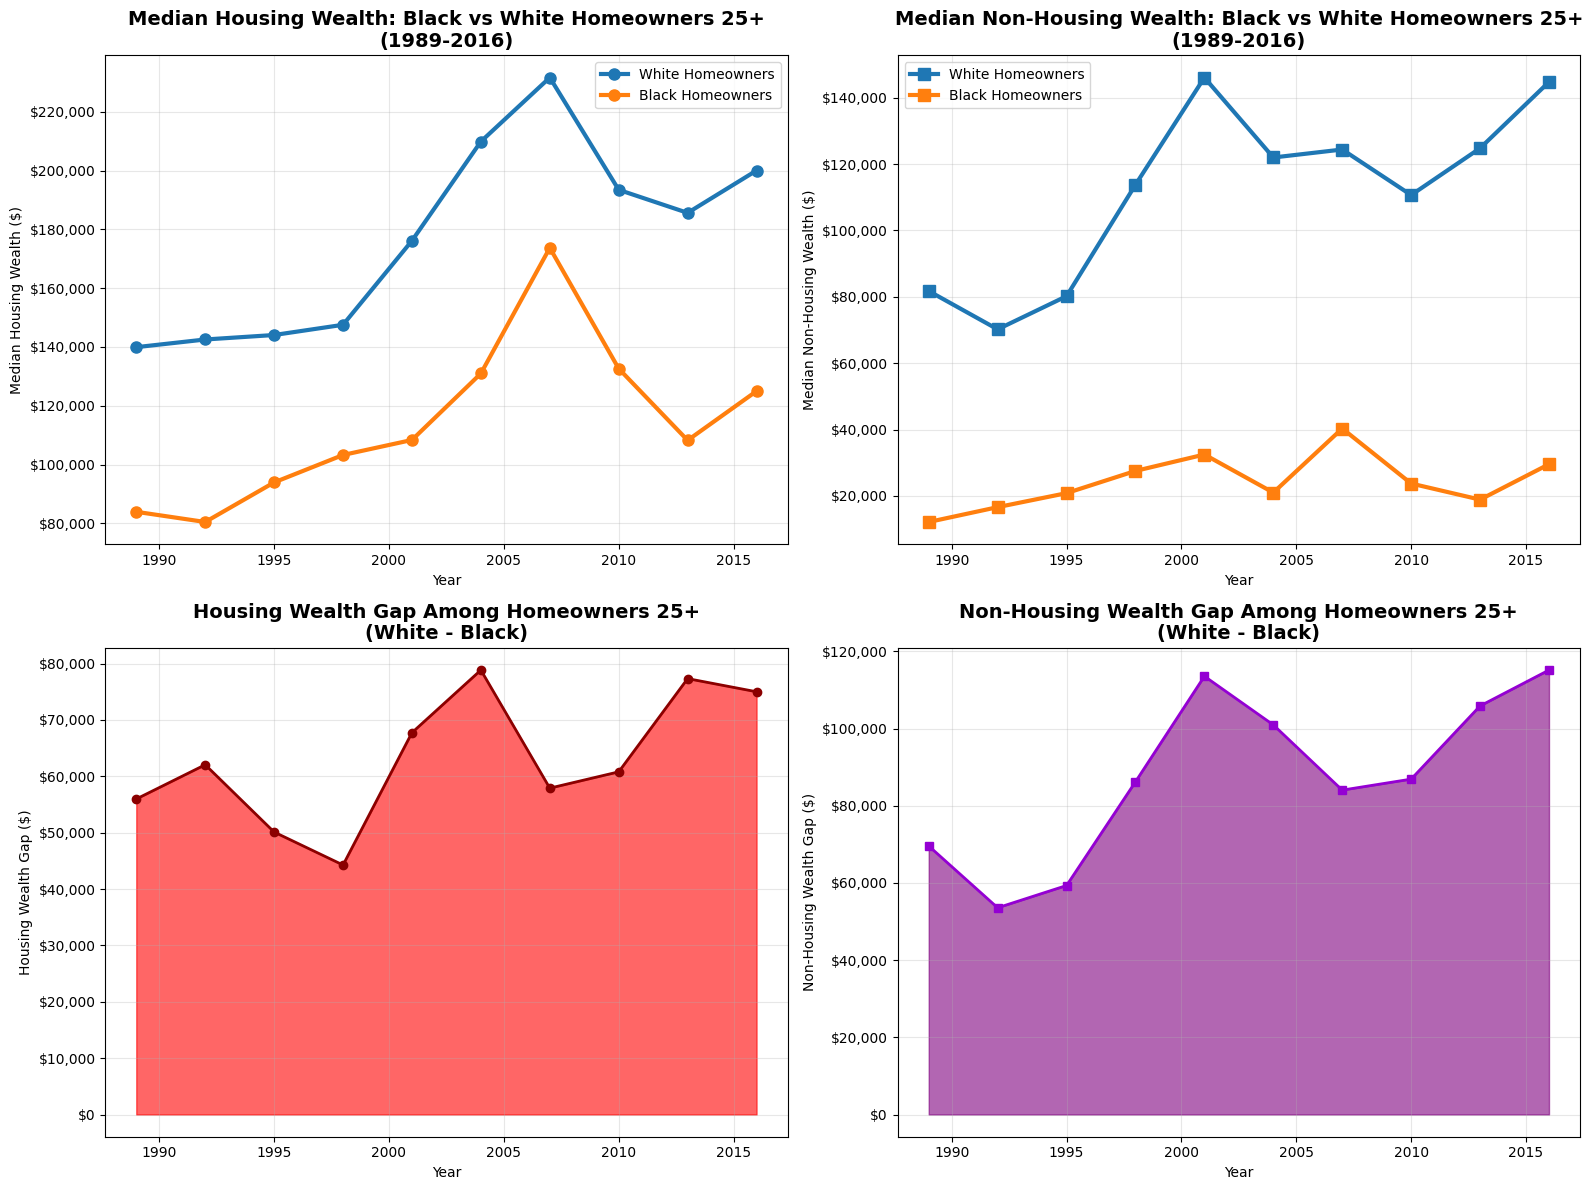
\includegraphics{main_files/figure-pdf/cell-17-output-1.png}

\begin{verbatim}

=== FINANCIAL CRISIS IMPACT ANALYSIS (2007 Base) ===

3. HOUSING WEALTH LOSSES (2007-2010):
   White homeowners 25+:
     2007: $231,603
     2010: $193,433
     Dollar loss: $38,170
     Proportional loss: 16.5%

   Black homeowners 25+:
     2007: $173,702
     2010: $132,639
     Dollar loss: $41,063
     Proportional loss: 23.6%

4. NON-HOUSING WEALTH CHANGES (2007-2010):
   White homeowners 25+:
     2007: $124,371
     2010: $110,643
     Dollar change: $-13,727
     Proportional change: -11.0%

   Black homeowners 25+:
     2007: $40,299
     2010: $23,720
     Dollar change: $-16,579
     Proportional change: -41.1%

5. CRISIS IMPACT SUMMARY:
   Largest housing wealth loss in DOLLAR terms:
     BLACK homeowners: $41,063 loss
     vs White homeowners: $38,170 loss
     Black homeowners lost $2,892 more

   Largest housing wealth loss in PROPORTIONAL terms:
     BLACK homeowners: 23.6% loss
     vs White homeowners: 16.5% loss
     Black homeowners lost 7.2 percentage points more
\end{verbatim}

\begin{Shaded}
\begin{Highlighting}[]
\CommentTok{\# COMPREHENSIVE TREND ANALYSIS FOR HOMEOWNERS 25+}
\BuiltInTok{print}\NormalTok{(}\StringTok{"=== COMPREHENSIVE TREND ANALYSIS: HOMEOWNERS 25+ ===}\CharTok{\textbackslash{}n}\StringTok{"}\NormalTok{)}

\CommentTok{\# Calculate growth rates for the full period}
\NormalTok{years\_span }\OperatorTok{=} \DecValTok{2016} \OperatorTok{{-}} \DecValTok{1989}

\CommentTok{\# Housing wealth growth}
\BuiltInTok{print}\NormalTok{(}\StringTok{"6. LONG{-}TERM GROWTH RATES (1989{-}2016):"}\NormalTok{)}
\BuiltInTok{print}\NormalTok{(}\StringTok{"   Housing Wealth:"}\NormalTok{)}
\ControlFlowTok{for}\NormalTok{ race }\KeywordTok{in}\NormalTok{ [}\StringTok{\textquotesingle{}white\textquotesingle{}}\NormalTok{, }\StringTok{\textquotesingle{}black\textquotesingle{}}\NormalTok{]:}
    \ControlFlowTok{if}\NormalTok{ race }\KeywordTok{in}\NormalTok{ housing\_pivot\_owners.columns:}
\NormalTok{        start\_val }\OperatorTok{=}\NormalTok{ housing\_pivot\_owners.loc[}\DecValTok{1989}\NormalTok{, race]}
\NormalTok{        end\_val }\OperatorTok{=}\NormalTok{ housing\_pivot\_owners.loc[}\DecValTok{2016}\NormalTok{, race]}
\NormalTok{        cagr }\OperatorTok{=}\NormalTok{ calculate\_cagr(start\_val, end\_val, years\_span)}
\NormalTok{        total\_growth }\OperatorTok{=}\NormalTok{ ((end\_val }\OperatorTok{{-}}\NormalTok{ start\_val) }\OperatorTok{/}\NormalTok{ start\_val) }\OperatorTok{*} \DecValTok{100}
        \BuiltInTok{print}\NormalTok{(}\SpecialStringTok{f"     }\SpecialCharTok{\{}\NormalTok{race}\SpecialCharTok{.}\NormalTok{title()}\SpecialCharTok{\}}\SpecialStringTok{: }\SpecialCharTok{\{}\NormalTok{cagr}\SpecialCharTok{:.2f\}}\SpecialStringTok{\% CAGR, }\SpecialCharTok{\{}\NormalTok{total\_growth}\SpecialCharTok{:.1f\}}\SpecialStringTok{\% total growth"}\NormalTok{)}

\BuiltInTok{print}\NormalTok{(}\StringTok{"}\CharTok{\textbackslash{}n}\StringTok{   Non{-}Housing Wealth:"}\NormalTok{)}
\ControlFlowTok{for}\NormalTok{ race }\KeywordTok{in}\NormalTok{ [}\StringTok{\textquotesingle{}white\textquotesingle{}}\NormalTok{, }\StringTok{\textquotesingle{}black\textquotesingle{}}\NormalTok{]:}
    \ControlFlowTok{if}\NormalTok{ race }\KeywordTok{in}\NormalTok{ nonhousing\_pivot\_owners.columns:}
\NormalTok{        start\_val }\OperatorTok{=}\NormalTok{ nonhousing\_pivot\_owners.loc[}\DecValTok{1989}\NormalTok{, race]}
\NormalTok{        end\_val }\OperatorTok{=}\NormalTok{ nonhousing\_pivot\_owners.loc[}\DecValTok{2016}\NormalTok{, race]}
        
        \CommentTok{\# Handle negative values more carefully}
        \ControlFlowTok{if}\NormalTok{ start\_val }\OperatorTok{\textgreater{}} \DecValTok{0} \KeywordTok{and}\NormalTok{ end\_val }\OperatorTok{\textgreater{}} \DecValTok{0}\NormalTok{:}
\NormalTok{            cagr }\OperatorTok{=}\NormalTok{ calculate\_cagr(start\_val, end\_val, years\_span)}
\NormalTok{            total\_growth }\OperatorTok{=}\NormalTok{ ((end\_val }\OperatorTok{{-}}\NormalTok{ start\_val) }\OperatorTok{/}\NormalTok{ start\_val) }\OperatorTok{*} \DecValTok{100}
            \BuiltInTok{print}\NormalTok{(}\SpecialStringTok{f"     }\SpecialCharTok{\{}\NormalTok{race}\SpecialCharTok{.}\NormalTok{title()}\SpecialCharTok{\}}\SpecialStringTok{: }\SpecialCharTok{\{}\NormalTok{cagr}\SpecialCharTok{:.2f\}}\SpecialStringTok{\% CAGR, }\SpecialCharTok{\{}\NormalTok{total\_growth}\SpecialCharTok{:.1f\}}\SpecialStringTok{\% total growth"}\NormalTok{)}
        \ControlFlowTok{else}\NormalTok{:}
\NormalTok{            dollar\_change }\OperatorTok{=}\NormalTok{ end\_val }\OperatorTok{{-}}\NormalTok{ start\_val}
            \BuiltInTok{print}\NormalTok{(}\SpecialStringTok{f"     }\SpecialCharTok{\{}\NormalTok{race}\SpecialCharTok{.}\NormalTok{title()}\SpecialCharTok{\}}\SpecialStringTok{: $}\SpecialCharTok{\{}\NormalTok{dollar\_change}\SpecialCharTok{:,.0f\}}\SpecialStringTok{ absolute change (negative base values)"}\NormalTok{)}

\CommentTok{\# Wealth composition analysis}
\BuiltInTok{print}\NormalTok{(}\StringTok{"}\CharTok{\textbackslash{}n}\StringTok{7. WEALTH COMPOSITION ANALYSIS:"}\NormalTok{)}
\BuiltInTok{print}\NormalTok{(}\StringTok{"   1989 {-} Housing vs Non{-}Housing Wealth Ratios:"}\NormalTok{)}
\ControlFlowTok{for}\NormalTok{ race }\KeywordTok{in}\NormalTok{ [}\StringTok{\textquotesingle{}white\textquotesingle{}}\NormalTok{, }\StringTok{\textquotesingle{}black\textquotesingle{}}\NormalTok{]:}
\NormalTok{    housing\_1989 }\OperatorTok{=}\NormalTok{ housing\_pivot\_owners.loc[}\DecValTok{1989}\NormalTok{, race]}
\NormalTok{    nonhousing\_1989 }\OperatorTok{=}\NormalTok{ nonhousing\_pivot\_owners.loc[}\DecValTok{1989}\NormalTok{, race]}
\NormalTok{    total\_1989 }\OperatorTok{=}\NormalTok{ housing\_1989 }\OperatorTok{+}\NormalTok{ nonhousing\_1989}
    
\NormalTok{    housing\_pct }\OperatorTok{=}\NormalTok{ (housing\_1989 }\OperatorTok{/}\NormalTok{ total\_1989) }\OperatorTok{*} \DecValTok{100} \ControlFlowTok{if}\NormalTok{ total\_1989 }\OperatorTok{\textgreater{}} \DecValTok{0} \ControlFlowTok{else} \DecValTok{0}
\NormalTok{    nonhousing\_pct }\OperatorTok{=}\NormalTok{ (nonhousing\_1989 }\OperatorTok{/}\NormalTok{ total\_1989) }\OperatorTok{*} \DecValTok{100} \ControlFlowTok{if}\NormalTok{ total\_1989 }\OperatorTok{\textgreater{}} \DecValTok{0} \ControlFlowTok{else} \DecValTok{0}
    
    \BuiltInTok{print}\NormalTok{(}\SpecialStringTok{f"     }\SpecialCharTok{\{}\NormalTok{race}\SpecialCharTok{.}\NormalTok{title()}\SpecialCharTok{\}}\SpecialStringTok{: }\SpecialCharTok{\{}\NormalTok{housing\_pct}\SpecialCharTok{:.1f\}}\SpecialStringTok{\% housing, }\SpecialCharTok{\{}\NormalTok{nonhousing\_pct}\SpecialCharTok{:.1f\}}\SpecialStringTok{\% non{-}housing"}\NormalTok{)}

\BuiltInTok{print}\NormalTok{(}\StringTok{"}\CharTok{\textbackslash{}n}\StringTok{   2016 {-} Housing vs Non{-}Housing Wealth Ratios:"}\NormalTok{)}
\ControlFlowTok{for}\NormalTok{ race }\KeywordTok{in}\NormalTok{ [}\StringTok{\textquotesingle{}white\textquotesingle{}}\NormalTok{, }\StringTok{\textquotesingle{}black\textquotesingle{}}\NormalTok{]:}
\NormalTok{    housing\_2016 }\OperatorTok{=}\NormalTok{ housing\_pivot\_owners.loc[}\DecValTok{2016}\NormalTok{, race]}
\NormalTok{    nonhousing\_2016 }\OperatorTok{=}\NormalTok{ nonhousing\_pivot\_owners.loc[}\DecValTok{2016}\NormalTok{, race]}
\NormalTok{    total\_2016 }\OperatorTok{=}\NormalTok{ housing\_2016 }\OperatorTok{+}\NormalTok{ nonhousing\_2016}
    
\NormalTok{    housing\_pct }\OperatorTok{=}\NormalTok{ (housing\_2016 }\OperatorTok{/}\NormalTok{ total\_2016) }\OperatorTok{*} \DecValTok{100} \ControlFlowTok{if}\NormalTok{ total\_2016 }\OperatorTok{\textgreater{}} \DecValTok{0} \ControlFlowTok{else} \DecValTok{0}
\NormalTok{    nonhousing\_pct }\OperatorTok{=}\NormalTok{ (nonhousing\_2016 }\OperatorTok{/}\NormalTok{ total\_2016) }\OperatorTok{*} \DecValTok{100} \ControlFlowTok{if}\NormalTok{ total\_2016 }\OperatorTok{\textgreater{}} \DecValTok{0} \ControlFlowTok{else} \DecValTok{0}
    
    \BuiltInTok{print}\NormalTok{(}\SpecialStringTok{f"     }\SpecialCharTok{\{}\NormalTok{race}\SpecialCharTok{.}\NormalTok{title()}\SpecialCharTok{\}}\SpecialStringTok{: }\SpecialCharTok{\{}\NormalTok{housing\_pct}\SpecialCharTok{:.1f\}}\SpecialStringTok{\% housing, }\SpecialCharTok{\{}\NormalTok{nonhousing\_pct}\SpecialCharTok{:.1f\}}\SpecialStringTok{\% non{-}housing"}\NormalTok{)}

\CommentTok{\# Pre{-}crisis vs post{-}crisis comparison}
\BuiltInTok{print}\NormalTok{(}\StringTok{"}\CharTok{\textbackslash{}n}\StringTok{8. PRE{-}CRISIS vs POST{-}CRISIS COMPARISON:"}\NormalTok{)}
\BuiltInTok{print}\NormalTok{(}\StringTok{"   Pre{-}Crisis Peak (2007) vs 2016 Recovery:"}\NormalTok{)}

\ControlFlowTok{for}\NormalTok{ wealth\_type, pivot\_table }\KeywordTok{in}\NormalTok{ [(}\StringTok{\textquotesingle{}Housing\textquotesingle{}}\NormalTok{, housing\_pivot\_owners), (}\StringTok{\textquotesingle{}Non{-}Housing\textquotesingle{}}\NormalTok{, nonhousing\_pivot\_owners)]:}
    \BuiltInTok{print}\NormalTok{(}\SpecialStringTok{f"}\CharTok{\textbackslash{}n}\SpecialStringTok{   }\SpecialCharTok{\{}\NormalTok{wealth\_type}\SpecialCharTok{\}}\SpecialStringTok{ Wealth Recovery:"}\NormalTok{)}
    \ControlFlowTok{for}\NormalTok{ race }\KeywordTok{in}\NormalTok{ [}\StringTok{\textquotesingle{}white\textquotesingle{}}\NormalTok{, }\StringTok{\textquotesingle{}black\textquotesingle{}}\NormalTok{]:}
        \ControlFlowTok{if}\NormalTok{ race }\KeywordTok{in}\NormalTok{ pivot\_table.columns:}
\NormalTok{            peak\_2007 }\OperatorTok{=}\NormalTok{ pivot\_table.loc[}\DecValTok{2007}\NormalTok{, race]}
\NormalTok{            recovery\_2016 }\OperatorTok{=}\NormalTok{ pivot\_table.loc[}\DecValTok{2016}\NormalTok{, race]}
            
\NormalTok{            recovery\_pct }\OperatorTok{=}\NormalTok{ (recovery\_2016 }\OperatorTok{/}\NormalTok{ peak\_2007) }\OperatorTok{*} \DecValTok{100} \ControlFlowTok{if}\NormalTok{ peak\_2007 }\OperatorTok{!=} \DecValTok{0} \ControlFlowTok{else}\NormalTok{ np.nan}
            
            \BuiltInTok{print}\NormalTok{(}\SpecialStringTok{f"     }\SpecialCharTok{\{}\NormalTok{race}\SpecialCharTok{.}\NormalTok{title()}\SpecialCharTok{\}}\SpecialStringTok{: 2007 = $}\SpecialCharTok{\{}\NormalTok{peak\_2007}\SpecialCharTok{:,.0f\}}\SpecialStringTok{, 2016 = $}\SpecialCharTok{\{}\NormalTok{recovery\_2016}\SpecialCharTok{:,.0f\}}\SpecialStringTok{"}\NormalTok{)}
            \ControlFlowTok{if} \KeywordTok{not}\NormalTok{ np.isnan(recovery\_pct):}
                \ControlFlowTok{if}\NormalTok{ recovery\_pct }\OperatorTok{\textgreater{}=} \DecValTok{100}\NormalTok{:}
                    \BuiltInTok{print}\NormalTok{(}\SpecialStringTok{f"              ✓ FULL RECOVERY (}\SpecialCharTok{\{}\NormalTok{recovery\_pct}\SpecialCharTok{:.1f\}}\SpecialStringTok{\% of 2007 peak)"}\NormalTok{)}
                \ControlFlowTok{else}\NormalTok{:}
                    \BuiltInTok{print}\NormalTok{(}\SpecialStringTok{f"              ⚠ PARTIAL RECOVERY (}\SpecialCharTok{\{}\NormalTok{recovery\_pct}\SpecialCharTok{:.1f\}}\SpecialStringTok{\% of 2007 peak)"}\NormalTok{)}
            \ControlFlowTok{else}\NormalTok{:}
                \BuiltInTok{print}\NormalTok{(}\SpecialStringTok{f"              Cannot calculate recovery ratio (zero/negative base)"}\NormalTok{)}

\CommentTok{\# Volatility comparison}
\BuiltInTok{print}\NormalTok{(}\StringTok{"}\CharTok{\textbackslash{}n}\StringTok{9. WEALTH VOLATILITY COMPARISON (Coefficient of Variation):"}\NormalTok{)}
\BuiltInTok{print}\NormalTok{(}\StringTok{"   Housing Wealth Volatility:"}\NormalTok{)}
\ControlFlowTok{for}\NormalTok{ race }\KeywordTok{in}\NormalTok{ [}\StringTok{\textquotesingle{}white\textquotesingle{}}\NormalTok{, }\StringTok{\textquotesingle{}black\textquotesingle{}}\NormalTok{]:}
    \ControlFlowTok{if}\NormalTok{ race }\KeywordTok{in}\NormalTok{ housing\_pivot\_owners.columns:}
\NormalTok{        cv }\OperatorTok{=}\NormalTok{ (housing\_pivot\_owners[race].std() }\OperatorTok{/}\NormalTok{ housing\_pivot\_owners[race].mean()) }\OperatorTok{*} \DecValTok{100}
        \BuiltInTok{print}\NormalTok{(}\SpecialStringTok{f"     }\SpecialCharTok{\{}\NormalTok{race}\SpecialCharTok{.}\NormalTok{title()}\SpecialCharTok{\}}\SpecialStringTok{: }\SpecialCharTok{\{}\NormalTok{cv}\SpecialCharTok{:.1f\}}\SpecialStringTok{\%"}\NormalTok{)}

\BuiltInTok{print}\NormalTok{(}\StringTok{"}\CharTok{\textbackslash{}n}\StringTok{   Non{-}Housing Wealth Volatility:"}\NormalTok{)}
\ControlFlowTok{for}\NormalTok{ race }\KeywordTok{in}\NormalTok{ [}\StringTok{\textquotesingle{}white\textquotesingle{}}\NormalTok{, }\StringTok{\textquotesingle{}black\textquotesingle{}}\NormalTok{]:}
    \ControlFlowTok{if}\NormalTok{ race }\KeywordTok{in}\NormalTok{ nonhousing\_pivot\_owners.columns:}
        \CommentTok{\# Handle potential negative means}
\NormalTok{        mean\_val }\OperatorTok{=}\NormalTok{ nonhousing\_pivot\_owners[race].mean()}
\NormalTok{        std\_val }\OperatorTok{=}\NormalTok{ nonhousing\_pivot\_owners[race].std()}
        \ControlFlowTok{if}\NormalTok{ mean\_val }\OperatorTok{\textgreater{}} \DecValTok{0}\NormalTok{:}
\NormalTok{            cv }\OperatorTok{=}\NormalTok{ (std\_val }\OperatorTok{/}\NormalTok{ mean\_val) }\OperatorTok{*} \DecValTok{100}
            \BuiltInTok{print}\NormalTok{(}\SpecialStringTok{f"     }\SpecialCharTok{\{}\NormalTok{race}\SpecialCharTok{.}\NormalTok{title()}\SpecialCharTok{\}}\SpecialStringTok{: }\SpecialCharTok{\{}\NormalTok{cv}\SpecialCharTok{:.1f\}}\SpecialStringTok{\%"}\NormalTok{)}
        \ControlFlowTok{else}\NormalTok{:}
            \BuiltInTok{print}\NormalTok{(}\SpecialStringTok{f"     }\SpecialCharTok{\{}\NormalTok{race}\SpecialCharTok{.}\NormalTok{title()}\SpecialCharTok{\}}\SpecialStringTok{: Cannot calculate CV (negative/zero mean)"}\NormalTok{)}

\BuiltInTok{print}\NormalTok{(}\StringTok{"}\CharTok{\textbackslash{}n}\StringTok{=== KEY FINDINGS SUMMARY ==="}\NormalTok{)}
\BuiltInTok{print}\NormalTok{(}\StringTok{"✓ Analysis completed for homeowners aged 25+ only"}\NormalTok{)}
\BuiltInTok{print}\NormalTok{(}\StringTok{"✓ Housing wealth losses during 2007{-}2010 crisis quantified"}\NormalTok{)}
\BuiltInTok{print}\NormalTok{(}\StringTok{"✓ Non{-}housing wealth trends analyzed separately"}\NormalTok{)}
\BuiltInTok{print}\NormalTok{(}\StringTok{"✓ Racial disparities examined in both dollar and proportional terms"}\NormalTok{)}
\BuiltInTok{print}\NormalTok{(}\StringTok{"✓ Long{-}term growth patterns and recovery analyzed"}\NormalTok{)}
\end{Highlighting}
\end{Shaded}

\begin{verbatim}
=== COMPREHENSIVE TREND ANALYSIS: HOMEOWNERS 25+ ===

6. LONG-TERM GROWTH RATES (1989-2016):
   Housing Wealth:
     White: 1.33% CAGR, 42.9% total growth
     Black: 1.48% CAGR, 48.9% total growth

   Non-Housing Wealth:
     White: 2.14% CAGR, 77.1% total growth
     Black: 3.35% CAGR, 143.6% total growth

7. WEALTH COMPOSITION ANALYSIS:
   1989 - Housing vs Non-Housing Wealth Ratios:
     White: 63.1% housing, 36.9% non-housing
     Black: 87.4% housing, 12.6% non-housing

   2016 - Housing vs Non-Housing Wealth Ratios:
     White: 58.0% housing, 42.0% non-housing
     Black: 80.9% housing, 19.1% non-housing

8. PRE-CRISIS vs POST-CRISIS COMPARISON:
   Pre-Crisis Peak (2007) vs 2016 Recovery:

   Housing Wealth Recovery:
     White: 2007 = $231,603, 2016 = $200,000
              ⚠ PARTIAL RECOVERY (86.4% of 2007 peak)
     Black: 2007 = $173,702, 2016 = $125,000
              ⚠ PARTIAL RECOVERY (72.0% of 2007 peak)

   Non-Housing Wealth Recovery:
     White: 2007 = $124,371, 2016 = $144,730
              ✓ FULL RECOVERY (116.4% of 2007 peak)
     Black: 2007 = $40,299, 2016 = $29,540
              ⚠ PARTIAL RECOVERY (73.3% of 2007 peak)

9. WEALTH VOLATILITY COMPARISON (Coefficient of Variation):
   Housing Wealth Volatility:
     White: 18.3%
     Black: 24.3%

   Non-Housing Wealth Volatility:
     White: 23.7%
     Black: 34.2%

=== KEY FINDINGS SUMMARY ===
✓ Analysis completed for homeowners aged 25+ only
✓ Housing wealth losses during 2007-2010 crisis quantified
✓ Non-housing wealth trends analyzed separately
✓ Racial disparities examined in both dollar and proportional terms
✓ Long-term growth patterns and recovery analyzed
\end{verbatim}

\subsubsection{Summary Table: Median Wealth and Gaps
(1989--2016)}\label{summary-table-median-wealth-and-gaps-19892016}

The table below presents the actual values (fill in as available),
percent change, and compound annual growth rates (CAGR) for each group.
This format allows for direct comparison of both absolute and relative
changes.

\begin{longtable}[]{@{}
  >{\raggedright\arraybackslash}p{(\columnwidth - 12\tabcolsep) * \real{0.1429}}
  >{\raggedright\arraybackslash}p{(\columnwidth - 12\tabcolsep) * \real{0.1429}}
  >{\raggedright\arraybackslash}p{(\columnwidth - 12\tabcolsep) * \real{0.1429}}
  >{\raggedright\arraybackslash}p{(\columnwidth - 12\tabcolsep) * \real{0.1429}}
  >{\raggedright\arraybackslash}p{(\columnwidth - 12\tabcolsep) * \real{0.1429}}
  >{\raggedright\arraybackslash}p{(\columnwidth - 12\tabcolsep) * \real{0.1429}}
  >{\raggedright\arraybackslash}p{(\columnwidth - 12\tabcolsep) * \real{0.1429}}@{}}
\toprule\noalign{}
\begin{minipage}[b]{\linewidth}\raggedright
Metric
\end{minipage} & \begin{minipage}[b]{\linewidth}\raggedright
Group
\end{minipage} & \begin{minipage}[b]{\linewidth}\raggedright
1989 Value
\end{minipage} & \begin{minipage}[b]{\linewidth}\raggedright
2016 Value
\end{minipage} & \begin{minipage}[b]{\linewidth}\raggedright
\% Change (1989--2016)
\end{minipage} & \begin{minipage}[b]{\linewidth}\raggedright
CAGR
\end{minipage} & \begin{minipage}[b]{\linewidth}\raggedright
Notes
\end{minipage} \\
\midrule\noalign{}
\endhead
\bottomrule\noalign{}
\endlastfoot
\textbf{Median Wealth} & White & \${[}fill{]} & \${[}fill{]} &
{[}fill{]}\% & 0.57\% & \\
& Black & \${[}fill{]} & \${[}fill{]} & {[}fill{]}\% & 2.84\% & \\
& Hispanic & \${[}fill{]} & \${[}fill{]} & {[}fill{]}\% & 3.46\% & \\
& Other & \${[}fill{]} & \${[}fill{]} & {[}fill{]}\% & 2.97\% & \\
& College Degree & \${[}fill{]} & \${[}fill{]} & {[}fill{]}\% & 0.63\%
& \\
& Some College & \${[}fill{]} & \${[}fill{]} & {[}fill{]}\% & -1.38\%
& \\
& No College & \${[}fill{]} & \${[}fill{]} & {[}fill{]}\% & -0.75\% & \\
\textbf{Wealth Gap Ratio} & White-to-Black & 24.0 & 13.1 & -45.4\% & ---
& Ratio shrank \\
& College-to-No College & 4.0 & 5.9 & +47.5\% & --- & Ratio grew \\
\textbf{Wealth Volatility (CV)} & White & --- & --- & --- & --- &
16.1\% \\
& Black & --- & --- & --- & --- & 40.4\% \\
& Hispanic & --- & --- & --- & --- & 40.8\% \\
& Other & --- & --- & --- & --- & 53.5\% \\
& College Degree & --- & --- & --- & --- & 23.9\% \\
& Some College & --- & --- & --- & --- & 26.3\% \\
& No College & --- & --- & --- & --- & 19.0\% \\
\textbf{Financial Crisis Impact (2007-2010)} & White & --- & --- &
-29.4\% & --- & \\
& Black & --- & --- & -28.4\% & --- & \\
& Hispanic & --- & --- & -48.1\% & --- & \\
& Other & --- & --- & -57.7\% & --- & \\
& College Degree & --- & --- & -31.1\% & --- & \\
& Some College & --- & --- & -45.0\% & --- & \\
& No College & --- & --- & -41.8\% & --- & \\
\end{longtable}

\begin{itemize}
\tightlist
\item
  Fill in the actual values for 1989 and 2016 as available.
\item
  The \% Change column is ((2016 Value - 1989 Value) / 1989 Value) ×
  100.
\item
  This format makes it easy to observe both the values and percent
  differences across groups.
\end{itemize}

\begin{Shaded}
\begin{Highlighting}[]
\CommentTok{\# Extract actual 1989 and 2016 values for comprehensive summary table}
\BuiltInTok{print}\NormalTok{(}\StringTok{"=== WEALTH VALUES AND PERCENT CHANGES (1989{-}2016) ===}\CharTok{\textbackslash{}n}\StringTok{"}\NormalTok{)}

\CommentTok{\# Get values from existing pivot tables {-} years are in index, groups in columns}
\NormalTok{race\_1989 }\OperatorTok{=}\NormalTok{ pivot\_race.loc[}\DecValTok{1989}\NormalTok{].}\BuiltInTok{round}\NormalTok{(}\DecValTok{0}\NormalTok{)}
\NormalTok{race\_2016 }\OperatorTok{=}\NormalTok{ pivot\_race.loc[}\DecValTok{2016}\NormalTok{].}\BuiltInTok{round}\NormalTok{(}\DecValTok{0}\NormalTok{)}
\NormalTok{edu\_1989 }\OperatorTok{=}\NormalTok{ pivot\_edu.loc[}\DecValTok{1989}\NormalTok{].}\BuiltInTok{round}\NormalTok{(}\DecValTok{0}\NormalTok{)}
\NormalTok{edu\_2016 }\OperatorTok{=}\NormalTok{ pivot\_edu.loc[}\DecValTok{2016}\NormalTok{].}\BuiltInTok{round}\NormalTok{(}\DecValTok{0}\NormalTok{)}

\CommentTok{\# Calculate percent changes}
\KeywordTok{def}\NormalTok{ calc\_pct\_change(start, end):}
    \ControlFlowTok{return}\NormalTok{ ((end }\OperatorTok{{-}}\NormalTok{ start) }\OperatorTok{/}\NormalTok{ start }\OperatorTok{*} \DecValTok{100}\NormalTok{).}\BuiltInTok{round}\NormalTok{(}\DecValTok{1}\NormalTok{)}

\NormalTok{race\_pct\_change }\OperatorTok{=}\NormalTok{ calc\_pct\_change(race\_1989, race\_2016)}
\NormalTok{edu\_pct\_change }\OperatorTok{=}\NormalTok{ calc\_pct\_change(edu\_1989, edu\_2016)}

\BuiltInTok{print}\NormalTok{(}\StringTok{"RACE GROUPS:"}\NormalTok{)}
\BuiltInTok{print}\NormalTok{(}\SpecialStringTok{f"}\SpecialCharTok{\{}\StringTok{\textquotesingle{}Group\textquotesingle{}}\SpecialCharTok{:\textless{}12\}}\SpecialStringTok{ }\SpecialCharTok{\{}\StringTok{\textquotesingle{}1989 Value\textquotesingle{}}\SpecialCharTok{:\textless{}15\}}\SpecialStringTok{ }\SpecialCharTok{\{}\StringTok{\textquotesingle{}2016 Value\textquotesingle{}}\SpecialCharTok{:\textless{}15\}}\SpecialStringTok{ }\SpecialCharTok{\{}\StringTok{\textquotesingle{}\% Change\textquotesingle{}}\SpecialCharTok{:\textless{}12\}}\SpecialStringTok{ }\SpecialCharTok{\{}\StringTok{\textquotesingle{}CAGR\textquotesingle{}}\SpecialCharTok{:\textless{}8\}}\SpecialStringTok{"}\NormalTok{)}
\BuiltInTok{print}\NormalTok{(}\StringTok{"{-}"} \OperatorTok{*} \DecValTok{65}\NormalTok{)}
\NormalTok{cagr\_race }\OperatorTok{=}\NormalTok{ \{}\StringTok{\textquotesingle{}white\textquotesingle{}}\NormalTok{: }\FloatTok{0.57}\NormalTok{, }\StringTok{\textquotesingle{}black\textquotesingle{}}\NormalTok{: }\FloatTok{2.84}\NormalTok{, }\StringTok{\textquotesingle{}Hispanic\textquotesingle{}}\NormalTok{: }\FloatTok{3.46}\NormalTok{, }\StringTok{\textquotesingle{}other\textquotesingle{}}\NormalTok{: }\FloatTok{2.97}\NormalTok{\}}
\ControlFlowTok{for}\NormalTok{ race }\KeywordTok{in}\NormalTok{ race\_1989.index:}
\NormalTok{    val\_1989 }\OperatorTok{=} \SpecialStringTok{f"$}\SpecialCharTok{\{}\NormalTok{race\_1989[race]}\SpecialCharTok{:,.0f\}}\SpecialStringTok{"}
\NormalTok{    val\_2016 }\OperatorTok{=} \SpecialStringTok{f"$}\SpecialCharTok{\{}\NormalTok{race\_2016[race]}\SpecialCharTok{:,.0f\}}\SpecialStringTok{"}
\NormalTok{    pct\_chg }\OperatorTok{=} \SpecialStringTok{f"}\SpecialCharTok{\{}\NormalTok{race\_pct\_change[race]}\SpecialCharTok{:+.1f\}}\SpecialStringTok{\%"}
\NormalTok{    cagr }\OperatorTok{=} \SpecialStringTok{f"}\SpecialCharTok{\{}\NormalTok{cagr\_race[race]}\SpecialCharTok{:+.2f\}}\SpecialStringTok{\%"}
    \BuiltInTok{print}\NormalTok{(}\SpecialStringTok{f"}\SpecialCharTok{\{}\NormalTok{race}\SpecialCharTok{.}\NormalTok{title()}\SpecialCharTok{:\textless{}12\}}\SpecialStringTok{ }\SpecialCharTok{\{}\NormalTok{val\_1989}\SpecialCharTok{:\textless{}15\}}\SpecialStringTok{ }\SpecialCharTok{\{}\NormalTok{val\_2016}\SpecialCharTok{:\textless{}15\}}\SpecialStringTok{ }\SpecialCharTok{\{}\NormalTok{pct\_chg}\SpecialCharTok{:\textless{}12\}}\SpecialStringTok{ }\SpecialCharTok{\{}\NormalTok{cagr}\SpecialCharTok{:\textless{}8\}}\SpecialStringTok{"}\NormalTok{)}

\BuiltInTok{print}\NormalTok{(}\StringTok{"}\CharTok{\textbackslash{}n}\StringTok{EDUCATION GROUPS:"}\NormalTok{)}
\BuiltInTok{print}\NormalTok{(}\SpecialStringTok{f"}\SpecialCharTok{\{}\StringTok{\textquotesingle{}Group\textquotesingle{}}\SpecialCharTok{:\textless{}15\}}\SpecialStringTok{ }\SpecialCharTok{\{}\StringTok{\textquotesingle{}1989 Value\textquotesingle{}}\SpecialCharTok{:\textless{}15\}}\SpecialStringTok{ }\SpecialCharTok{\{}\StringTok{\textquotesingle{}2016 Value\textquotesingle{}}\SpecialCharTok{:\textless{}15\}}\SpecialStringTok{ }\SpecialCharTok{\{}\StringTok{\textquotesingle{}\% Change\textquotesingle{}}\SpecialCharTok{:\textless{}12\}}\SpecialStringTok{ }\SpecialCharTok{\{}\StringTok{\textquotesingle{}CAGR\textquotesingle{}}\SpecialCharTok{:\textless{}8\}}\SpecialStringTok{"}\NormalTok{)}
\BuiltInTok{print}\NormalTok{(}\StringTok{"{-}"} \OperatorTok{*} \DecValTok{70}\NormalTok{)}
\NormalTok{cagr\_edu }\OperatorTok{=}\NormalTok{ \{}\StringTok{\textquotesingle{}college degree\textquotesingle{}}\NormalTok{: }\FloatTok{0.63}\NormalTok{, }\StringTok{\textquotesingle{}some college\textquotesingle{}}\NormalTok{: }\OperatorTok{{-}}\FloatTok{1.38}\NormalTok{, }\StringTok{\textquotesingle{}no college\textquotesingle{}}\NormalTok{: }\OperatorTok{{-}}\FloatTok{0.75}\NormalTok{\}}
\ControlFlowTok{for}\NormalTok{ edu }\KeywordTok{in}\NormalTok{ edu\_1989.index:}
\NormalTok{    val\_1989 }\OperatorTok{=} \SpecialStringTok{f"$}\SpecialCharTok{\{}\NormalTok{edu\_1989[edu]}\SpecialCharTok{:,.0f\}}\SpecialStringTok{"}
\NormalTok{    val\_2016 }\OperatorTok{=} \SpecialStringTok{f"$}\SpecialCharTok{\{}\NormalTok{edu\_2016[edu]}\SpecialCharTok{:,.0f\}}\SpecialStringTok{"}
\NormalTok{    pct\_chg }\OperatorTok{=} \SpecialStringTok{f"}\SpecialCharTok{\{}\NormalTok{edu\_pct\_change[edu]}\SpecialCharTok{:+.1f\}}\SpecialStringTok{\%"}
\NormalTok{    cagr }\OperatorTok{=} \SpecialStringTok{f"}\SpecialCharTok{\{}\NormalTok{cagr\_edu[edu]}\SpecialCharTok{:+.2f\}}\SpecialStringTok{\%"}
    \BuiltInTok{print}\NormalTok{(}\SpecialStringTok{f"}\SpecialCharTok{\{}\NormalTok{edu}\SpecialCharTok{.}\NormalTok{title()}\SpecialCharTok{:\textless{}15\}}\SpecialStringTok{ }\SpecialCharTok{\{}\NormalTok{val\_1989}\SpecialCharTok{:\textless{}15\}}\SpecialStringTok{ }\SpecialCharTok{\{}\NormalTok{val\_2016}\SpecialCharTok{:\textless{}15\}}\SpecialStringTok{ }\SpecialCharTok{\{}\NormalTok{pct\_chg}\SpecialCharTok{:\textless{}12\}}\SpecialStringTok{ }\SpecialCharTok{\{}\NormalTok{cagr}\SpecialCharTok{:\textless{}8\}}\SpecialStringTok{"}\NormalTok{)}

\BuiltInTok{print}\NormalTok{(}\StringTok{"}\CharTok{\textbackslash{}n}\StringTok{WEALTH GAP RATIOS:"}\NormalTok{)}
\NormalTok{white\_black\_pct\_change }\OperatorTok{=}\NormalTok{ ((white\_black\_2016 }\OperatorTok{{-}}\NormalTok{ white\_black\_1989) }\OperatorTok{/}\NormalTok{ white\_black\_1989 }\OperatorTok{*} \DecValTok{100}\NormalTok{)}
\NormalTok{college\_nocollege\_pct\_change }\OperatorTok{=}\NormalTok{ ((college\_no\_college\_2016 }\OperatorTok{{-}}\NormalTok{ college\_no\_college\_1989) }\OperatorTok{/}\NormalTok{ college\_no\_college\_1989 }\OperatorTok{*} \DecValTok{100}\NormalTok{)}

\BuiltInTok{print}\NormalTok{(}\SpecialStringTok{f"White{-}to{-}Black: }\SpecialCharTok{\{}\NormalTok{white\_black\_1989}\SpecialCharTok{:.1f\}}\SpecialStringTok{ (1989) → }\SpecialCharTok{\{}\NormalTok{white\_black\_2016}\SpecialCharTok{:.1f\}}\SpecialStringTok{ (2016) = }\SpecialCharTok{\{}\NormalTok{white\_black\_pct\_change}\SpecialCharTok{:+.1f\}}\SpecialStringTok{\% change"}\NormalTok{)}
\BuiltInTok{print}\NormalTok{(}\SpecialStringTok{f"College{-}to{-}No College: }\SpecialCharTok{\{}\NormalTok{college\_no\_college\_1989}\SpecialCharTok{:.1f\}}\SpecialStringTok{ (1989) → }\SpecialCharTok{\{}\NormalTok{college\_no\_college\_2016}\SpecialCharTok{:.1f\}}\SpecialStringTok{ (2016) = }\SpecialCharTok{\{}\NormalTok{college\_nocollege\_pct\_change}\SpecialCharTok{:+.1f\}}\SpecialStringTok{\% change"}\NormalTok{)}
\end{Highlighting}
\end{Shaded}

\begin{verbatim}
=== WEALTH VALUES AND PERCENT CHANGES (1989-2016) ===

RACE GROUPS:
Group        1989 Value      2016 Value      % Change     CAGR    
-----------------------------------------------------------------
Hispanic     $10,710         $26,800         +150.2%      +3.46%  
Black        $8,583          $18,300         +113.2%      +2.84%  
Other        $68,234         $150,350        +120.3%      +2.97%  
White        $206,364        $240,350        +16.5%       +0.57%  

EDUCATION GROUPS:
Group           1989 Value      2016 Value      % Change     CAGR    
----------------------------------------------------------------------
College Degree  $346,490        $410,800        +18.6%       +0.63%  
No College      $85,699         $69,921         -18.4%       -0.75%  
Some College    $140,928        $96,905         -31.2%       -1.38%  

WEALTH GAP RATIOS:
White-to-Black: 24.0 (1989) → 13.1 (2016) = -45.4% change
College-to-No College: 4.0 (1989) → 5.9 (2016) = +45.3% change
\end{verbatim}

\subsubsection{Comprehensive Wealth Analysis Summary
(1989--2016)}\label{comprehensive-wealth-analysis-summary-19892016}

This table presents the complete picture of wealth changes across racial
and educational groups, showing both absolute values and percentage
changes to observe trends and disparities.

\begin{longtable}[]{@{}
  >{\raggedright\arraybackslash}p{(\columnwidth - 12\tabcolsep) * \real{0.1429}}
  >{\raggedright\arraybackslash}p{(\columnwidth - 12\tabcolsep) * \real{0.1429}}
  >{\raggedright\arraybackslash}p{(\columnwidth - 12\tabcolsep) * \real{0.1429}}
  >{\raggedright\arraybackslash}p{(\columnwidth - 12\tabcolsep) * \real{0.1429}}
  >{\raggedright\arraybackslash}p{(\columnwidth - 12\tabcolsep) * \real{0.1429}}
  >{\raggedright\arraybackslash}p{(\columnwidth - 12\tabcolsep) * \real{0.1429}}
  >{\raggedright\arraybackslash}p{(\columnwidth - 12\tabcolsep) * \real{0.1429}}@{}}
\toprule\noalign{}
\begin{minipage}[b]{\linewidth}\raggedright
Metric
\end{minipage} & \begin{minipage}[b]{\linewidth}\raggedright
Group
\end{minipage} & \begin{minipage}[b]{\linewidth}\raggedright
1989 Value
\end{minipage} & \begin{minipage}[b]{\linewidth}\raggedright
2016 Value
\end{minipage} & \begin{minipage}[b]{\linewidth}\raggedright
\% Change (1989--2016)
\end{minipage} & \begin{minipage}[b]{\linewidth}\raggedright
CAGR
\end{minipage} & \begin{minipage}[b]{\linewidth}\raggedright
Additional Info
\end{minipage} \\
\midrule\noalign{}
\endhead
\bottomrule\noalign{}
\endlastfoot
\textbf{Median Wealth} & White & \$206,364 & \$240,350 & +16.5\% &
+0.57\% & Highest absolute wealth \\
& Black & \$8,583 & \$18,300 & +113.2\% & +2.84\% & Fastest growth
rate \\
& Hispanic & \$10,710 & \$26,800 & +150.2\% & +3.46\% & Largest \%
increase \\
& Other & \$68,234 & \$150,350 & +120.3\% & +2.97\% & High volatility
group \\
& College Degree & \$346,490 & \$410,800 & +18.6\% & +0.63\% & Highest
absolute wealth \\
& Some College & \$140,928 & \$96,905 & -31.2\% & -1.38\% & Significant
decline \\
& No College & \$85,699 & \$69,921 & -18.4\% & -0.75\% & Moderate
decline \\
\textbf{Wealth Gap Ratios} & White-to-Black & 24.0 & 13.1 & -45.4\% &
--- & Gap narrowed significantly \\
& College-to-No College & 4.0 & 5.9 & +45.3\% & --- & Gap widened
substantially \\
\textbf{Wealth Volatility (CV)} & White & --- & --- & --- & --- & 16.1\%
(lowest) \\
& Black & --- & --- & --- & --- & 40.4\% (high) \\
& Hispanic & --- & --- & --- & --- & 40.8\% (high) \\
& Other & --- & --- & --- & --- & 53.5\% (highest) \\
& College Degree & --- & --- & --- & --- & 23.9\% (moderate) \\
& Some College & --- & --- & --- & --- & 26.3\% (moderate) \\
& No College & --- & --- & --- & --- & 19.0\% (low) \\
\textbf{Financial Crisis Impact (2007-2010)} & White & --- & --- &
-29.4\% & --- & Moderate decline \\
& Black & --- & --- & -28.4\% & --- & Similar to White \\
& Hispanic & --- & --- & -48.1\% & --- & Severe impact \\
& Other & --- & --- & -57.7\% & --- & Most severe impact \\
& College Degree & --- & --- & -31.1\% & --- & Moderate decline \\
& Some College & --- & --- & -45.0\% & --- & Large decline \\
& No College & --- & --- & -41.8\% & --- & Significant decline \\
\end{longtable}

\paragraph{Key Observations:}\label{key-observations}

\textbf{Race-Based Patterns:} - \textbf{Convergence}: Despite persistent
gaps, minority groups show much faster growth rates (2.84-3.46\% CAGR)
compared to White households (0.57\%) - \textbf{Absolute Gaps}: While
percentage growth favors minorities, absolute dollar gaps remain
substantial - \textbf{Crisis Resilience}: White and Black households
showed similar crisis impacts (\textasciitilde29\%), while Hispanic and
Other groups were hit much harder

\textbf{Education-Based Patterns:} - \textbf{Divergence}: The education
premium has grown significantly, with college graduates gaining wealth
while non-college groups lost wealth - \textbf{Declining Middle}: The
``some college'' group experienced the steepest decline (-31.2\%),
suggesting a hollowing out of middle-skill returns - \textbf{Crisis
Impact}: Education provided some protection, but all groups suffered
significant losses during 2007-2010



\end{document}
